\documentclass[a4paper,openany]{article} 
\addtolength{\hoffset}{-2.25cm}
\addtolength{\textwidth}{4.5cm}
\addtolength{\voffset}{-3.25cm}
\addtolength{\textheight}{5cm}
\setlength{\parskip}{0pt}
\setlength{\parindent}{0in}

%----------------------------------------------------------------------------------------
%	PACKAGES AND OTHER DOCUMENT CONFIGURATIONS
%----------------------------------------------------------------------------------------

\usepackage{blindtext} % Package to generate dummy text
\usepackage{charter} % Use the Charter font
\usepackage[utf8]{inputenc} % Use UTF-8 encoding
\usepackage{microtype} % Slightly tweak font spacing for aesthetics
\usepackage[italian]{babel} % Language hyphenation and typographical rules
\usepackage{amsthm, amsmath, amssymb} % Mathematical typesetting
\usepackage{float} % Improved interface for floating objects
\usepackage[final, colorlinks = true, 
            linkcolor = black, 
            citecolor = black]{hyperref} % For hyperlinks in the PDF
\usepackage{graphicx, multicol} % Enhanced support for graphics
\usepackage{xcolor} % Driver-independent color extensions
\usepackage{marvosym, wasysym} % More symbols
\usepackage{rotating} % Rotation tools
\usepackage{censor} % Facilities for controlling restricted text
\usepackage{listings, style/lstlisting} % Environment for non-formatted code, !uses style file!
\usepackage{pseudocode} % Environment for specifying algorithms in a natural way
\usepackage{style/avm} % Environment for f-structures, !uses style file!
\usepackage{booktabs} % Enhances quality of tables
\usepackage{tikz-qtree} % Easy tree drawing tool
\tikzset{every tree node/.style={align=center,anchor=north},
         level distance=2cm} % Configuration for q-trees
\usepackage{style/btree} % Configuration for b-trees and b+-trees, !uses style file!
\usepackage[backend=biber,style=numeric,
            sorting=nyt]{biblatex} % Complete reimplementation of bibliographic facilities
\addbibresource{ecl.bib}
\usepackage{csquotes} % Context sensitive quotation facilities
\usepackage[yyyymmdd]{datetime} % Uses YEAR-MONTH-DAY format for dates
\renewcommand{\dateseparator}{-} % Sets dateseparator to '-'
\usepackage{fancyhdr} % Headers and footers
\pagestyle{fancy} % All pages have headers and footers
\fancyhead{}\renewcommand{\headrulewidth}{0pt} % Blank out the default header
\fancyfoot[L]{} % Custom footer text
\fancyfoot[C]{} % Custom footer text
\fancyfoot[R]{\thepage} % Custom footer text
\newcommand{\note}[1]{\marginpar{\scriptsize \textcolor{red}{#1}}} % Enables comments in red on margin



\usepackage{amsmath}
\usepackage{amsfonts}
\usepackage{tcolorbox}
%----------------------------------------------------------------------------------------

\tcbuselibrary{theorems}
\usepackage{listings}
\usepackage{color}
\usepackage[ruled,vlined,longend,linesnumbered]{algorithm2e}

\definecolor{darkgreen}{rgb}{0,0.6,0}
\definecolor{gray}{rgb}{0.5,0.5,0.5}
\definecolor{mauve}{rgb}{0.58,0,0.82}

\newtcbtheorem[]{teorema}{}%
{colback=gray!15,colframe=gray!70}{th}

\lstset{frame=tb,
  language=java,
  aboveskip=3mm,
  belowskip=3mm,
  showstringspaces=false,
  columns=flexible,
  basicstyle={\small\ttfamily},
  numbers=left,
  numberstyle=\tiny\color{gray},
  keywordstyle=\color{blue},
  commentstyle=\color{darkgreen},
  stringstyle=\color{mauve},
  breaklines=true,
  breakatwhitespace=true,
  tabsize=3
}

\begin{document}

%-------------------------------
%	TITLE SECTION
%-------------------------------

\fancyhead[C]{}
\hrule \medskip % Upper rule
\begin{minipage}{0.295\textwidth} 
\raggedright
\footnotesize
Andrei Gabriel Taraboi \hfill\\   
\hfill\\
\end{minipage}
\begin{minipage}{0.4\textwidth} 
\centering 
\large 
Teoria della Computazione\\ 
\normalsize 
\end{minipage}
\begin{minipage}{0.295\textwidth} 
\raggedleft
\hfill\\
\end{minipage}
\medskip\hrule 
\bigskip

\raggedbottom
%-------------------------------
%	CONTENTS
%-------------------------------
\tableofcontents
\newpage
\part{Lezioni frontali - Bonizzoni}
\section{Lezione del 6 ottobre - Bonizzoni}
\subsection{Problemmi di decisione}
La teoria della \textbf{complessità computazionale} si riferisce a varie \textbf{classi di complessità} che classificano, in un primo approccio, \textit{problemi decisionali} descritti da funzioni binarie che hanno in input una stringa sull'alfabeto $\{0,1\}$ e restituiscono un bit (0,1). 
Sia $\Pi$ un problema di decisione 
\begin{itemize}
    \item \textbf{input}: $x$ istanza, $|x| = n$ 
    \item \textbf{output}: $0$ (NO), $1$ (YES)
\end{itemize} La funzione $f_{\Pi}$ associata a $\Pi$ è: $f_{\Pi} : \{0,1\}^* \to \{0,1\}$. Questo perché le macchine di Turing ragionano in binario. 

\textbf{Esistono problemi che si è dimostrato non essere risolvibili in tempo efficiente.}\\ Tra le classi abbiamo i \textbf{problemi NP} e \textbf{problemi P}. Inoltre i problemi NP sono a loro volta classificabili tra loro cercando i più difficili, ottenendo \textbf{problemi NP-hard} e \textbf{problemi NP-complete} (esistono varie dimostrazioni per la \textit{NP-completezza}). 

\subsection{Tempo di calcolo di una TM} 
 Sia $T:\mathbb{N} \to \mathbb{N}$ una funzione calcolabile da TM e $L_\Pi$ un linguaggio di decisione (dove $\pi$ sta per problema e di decisione ci ricorda che il risultato sarà binario), allora una \textbf{TM deterministica} $M$ accetta (risponde $1$, YES) $L_\Pi$ in tempo $T(n)$ se, $\forall x\in L_\pi$, con $|x|=n$, $M$ accetta $x$ in $T(n)$ mosse o configurazioni.
 
 Un \textbf{problema di decisione} $\pi$ riceve in input un'istanza $x$ e l'output è: 
 \begin{itemize} 
    \item 0 che vuole dire \textit{no} 
    \item 1 che vuole dire \textit{yes} 
\end{itemize} 

Un linguaggio $L_\Pi$ restituisce 1 per tutti gli $x$ che appartengono al linguaggio. Quindi $L_\Pi$ è l'insieme degli input di $\pi$ su cui l'output è 1.\\ 
La \textbf{funzione associata al problema} si chiama $f_\pi$ ed è la funzione che dato un input restituisce 1 sse l'input appartiene al $L_\Pi$.  \\
La classe dei linguaggi di decisione accettati in tempo $T(n)=cn^p \quad p\in\mathbb{N}, \quad p\neq 0$ da una TM deterministica è detta \textbf{classe P}. \\ 
Potenzialmente $p$ potrebbe anche non essere un intero in quanto si potrebbero avere tempi frazionari e non polinomiali. Si definisce che $L_\Pi$ è accettato da una TM in tempo $T(n)$ se $\exists \,\,T :\mathbb{N}\to \mathbb{N}$ calcolabile da TM e $\forall x\in L_\Pi$, con $|x|=n$, la TM accetta $x$ e risponde 1 (\textit{yes}) in al più $T(n)$ mosse di calcolo (dette anche configurazioni).\\ 

Se $y \notin L_\Pi$, siccome è stato fissato un limite di tempo $T(n)$, allora è possibile costruire una macchina $M'$ che accetta il complemento del linguaggio $L_\Pi$. Infatti $\exists M' |$ se $y \notin L_{\Pi}$ è input, questa impiega $T(n)$ per dire che $y \notin L_{\Pi}$. \\
Complemento di $L_\Pi = \{y \: | \: f_\Pi (y) = 0\}$ \\
La macchina $M'$ simula $M$ su input $y$ e se dopo $T(n)$ mosse su input $y$, con $|y| = n$ non è stata accettato $y$, allora $M'$ va nello stato finale con $0$ in output.

\subsection{Macchina RAM}
Nel caso del modello della macchina RAM si ha la stessa situazione con però $T(n)$ \textbf{istruzioni RAM} e si dice che $L_\Pi$ è accettato dalla macchina RAM (si può dire che è anche deciso dell'algoritmo A della macchina RAM). In caso contrario la macchina RAM restituisce \textit{no}, in quanto si parla di ``decisione'' oltre che di ``accettazione'' (a differenza della TM, dove però si può ottenere lo stesso discorso parlando di TM complementare $M'$, che in $T(n)$ mi risponderà yes alla richiesta che un input non appartenga a $L_\Pi$, altrimenti bisogna fissare un limite di tempo per ottenere yes).\\ È dimostrabile che se $L_\Pi$ è accettabile in tempo polinomiale allora nello stesso tempo è anche decidibile.\\ La differenza tra accettazione e decisione sarà fondamentale nel \textbf{modello non deterministico}.  

Si ricordi che il \textbf{modello RAM (\textit{Random Access Machine})} è usato per studiare il tempo di calcolo di uno pseudocodice. È un modello teorico (una macchina teorica ``simile'' a quelle reali) dotato di istruzioni come \textit{load, store, add, etc$\ldots$} dove un codice (ipoteticamente in qualsiasi linguaggio incluso lo pseudocodice) viene tradotto in una sorta di linguaggio macchina (linguaggio RAM), dove $n$ è un intero rappresentante il numero di istruzioni RAM necessarie per ottenere l'output ($n$ è detto \textbf{tempo uniforme}). Sul linguaggio RAM si può studiare anche lo spazio calcolato come numero di bit necessari per la computazione (è detto \textbf{costo logaritmico}). In questo secondo punto il costo di un'istruzione, come ad esempio \textit{load(n)}, è logaritmico rispetto all'operando $n$ ($\,\log_2 n$), studia quindi la \emph{dimensione} dell'input.  

\raggedbottom
\section{Lezione del 12 ottobre - Bonizzoni }
Abbiamo come obiettivo principale quello di classificare i problemi sulla base della loro difficoltà di soluzione mediante le macchine di calcolo. La \textit{difficoltà} viene stimata rispetto all'uso delle risorse di calcolo quali tempo e spazio.

La complessità, nel definire le classi dei problemi ha preso in considerazione, come prima classe, i problemi di decisioni.
Quest'ultimi, ricordiamo, sono descritti da funzioni binarie che hanno in input una stringa su alfabeto $\{0,1\}$ e restituiscono un bit 0/1. Tipicamente il problema è identificato come $\Pi$, che riceve in input $x$ e risponde 0 (no) oppure 1 (YES), relativo alla esistenza di una certa soluzione.

\subsection{Problema di ottimizzazione}
Sia $\Pi$, tipicamente rappresentano un problema per cui si vuole trovare un output dato un input che ottimizza la soluzione. L'output tipicamente ottimizza una misura, che dipende dalla dimensione dell'input, può essere un problema di minimo o di massimo.\\
Introducendo un nuovo parametro $k$, possiamo trasformare il nostro problema in un problema di decisione, sia quindi un output $y$, posso chiedere se $\exists y \mbox{ tale che } |y| = K$.

Mediante un problema di decisione possiamo trovare la misura ottima di una determinata soluzione eseguente diverse chiamate.

\subsubsection{Esempio problema di ottimizzazione}
Prendo il problema $\Pi$ \emph{vertex-cover}. Come input si ha un grafo $G=(V,E)$ e un intero $k$ e come output 0/1.
Essendo un problema di decisione, e si cerca di capire se $\exists\, V'\subseteq V$ tale che $V'$ è una copertura di $G$. Il sottoinsieme è copertura di un grafo quando $forall\, e\in E$ almeno un estremo dell'arco $e=(u,v)$ è in $V'$. \\
La copertura con il minor numero di vertici è detta \textbf{minima copertura}.\\ 
Il problema \emph{vertex-cover} chiede se esiste una copertura del grafo di dimensione $k$. È quindi diventa un \textbf{problema di decisione}. Qualora trovassi una copertura di cardinalità minore di $k$ mi basterà aggiungere vertici arbitrari fino al raggiungimento di $k$. Ovviamente può non esistere una copertura di cardinalità $k$.\\ 
\subsection{NDTM}
Sapendo che un \textbf{algoritmo intrattabile} non risolve in modo efficiente tutti gli input. Bisognerà trovare un modo per capire se un algoritmo è \textbf{intrattabile}.\\
Studiamo ora il tempo di calcolo di una \textbf{macchina di Turing non deterministica (\textit{NTDM})}: \\ 
Sia $T:\mathbb{N}\to\mathbb{N}$ una funziona calcolabile da TM. Dato $L_\Pi$ un linguaggio di decisione allora una $NDTM$ nondeterministica  $M$ accetta $L_\Pi$ in tempo $T(n)$ se per ogni $x$ in $L_\Pi$ ,con $|x|=n$,  $M$ accetta $x$ in $T(n)$ mosse (o configurazioni).\\ 
    
Quindi la \textbf{classe NP} è la classe dei linguaggi di decisione accettati in tempo $T(n)=cn^p,\quad p\in \mathbb{N}$ da una $NDTM$. \\
Per poter dare una definizione alternativa di NP usando gli algoritmi con certificato, bisogna prima introdurre quest'ultimi.

\subsection{Algoritmo con Certificato}
La classe $P$, polinomiale, sono i linguaggi accettati da un algoritmo polinomiale in tempo. I problemi invece $NP$, non polinomiali, sono linguaggi accettati da un algoritmo, che fanno uso di un \textit{ certificati}, polinomiale in tempo. 

Un algoritmo con certificato/verificatore è quindi un algoritmo di verifica se $x \in L$ usando y, dove $y$ è una stringa aggiuntiva che viene utilizzata insieme all'input che ci aiuta a dimostrare che $x$ appartiene al linguaggio $L$.\\
Quindi per un problema \textbf{NP} con certificato non posso trovare soluzione in tempo polinomiale ma posso verificare una soluzione data in tempo polinomiale.\\ 

\subsubsection{Definizione alternativa di NP}
Sia $L_\Pi$ un linguaggio di decisione, $T:n\to n$ una funzione calcolabile, $y$ una stringa di lunghezza polinomiale nell'input, allora un algoritmo $A$ con certificato accetta $L_\Pi$ in tempo $t(n)$ se per ogni $x$ in $L_\Pi$, con $|x|=n$, A termina su input $(x,y)$ dopo $t(|x|)$ passi di calcolo (istruzioni eseguite) producendo 1 in output.
  
Quindi la \textbf{classe NP} è la classe dei linguaggi (o problemi) di decisione accettati in tempo $T(n)=cn^p, \quad p\in\mathbb{N}$ da un algoritmo $A$ certificato

%spiega vertex-cover
Riprendendo l'esempio di algoritmo di ottimizzazione, affermiamo che \emph{vertex-cover} decisionale è nella classe \textbf{NP} con certificato e, in questo caso, il parametro $y$ è la dimostrazione che posso dare risposta affermativa, per esempio la certezza di avere un sottoinsieme di vertici che effettivamente copre tutto il grafo, quindi $y=V''\subseteq V$ tale per cui $V''$ copre $G$ con cardinalità $k$. 


Bisogna capire come trovare e come usare $y$, sapendo che $A$ lavora in tempo polinomiale e che la lunghezza di $y$ è polinomiale in dimensione di $x$.\\ Vedendo che la cardinalità di $y$ è minore di $k$ l'algoritmo A verifica che con i vertici passati con $y$ si è in grado di rispondere al problema in modo affermativo, problema che ha in input $G$ e $k$. In poche parole $A$, per ogni arco, esamina se ogni estremo è in $y$ e, se tutti gli archi hanno un estremo in $y$ allora si ha che usando $y$ si è in grado di verificare l'input $G, k$ è \textbf{accettato}. Questa verifica è in tempo polinomiale e si ha che $|y|=\mathcal{O}(|G,k|)$, soprattutto se $|y|$ è una costante.\\ 
Ad oggi non si è dimostrato che \emph{vertex-cover} si risolvibile in tempo polinomiale. È quindi un problema \textbf{NP-hard}.\\ \newline

\textbf{P} è vista come sottoclasse la \textbf{NP} dove i problemi di decisione sono risolvibili in tempo polinomiale anche senza certificato. Per dimostrare che $P\subseteq NP$ devo far vedere che ogni $L_\Pi\in P$ ammette un algoritmo $A$ con certificato in tempo polinomiale. Ma questo è vero perché $L_\Pi$ è accettato da un algoritmo $A$, in tempo polinomiale con $y=\emptyset$ e quindi $y$ non è necessario.\\
Si ha quindi che $P\subseteq NP$. 
\section{Riduzioni polinomiali}
Si hanno alcuni problemi che sono in grado di risolvere qualunque problema di decisione in \textbf{NP}. Serviranno prima le definizioni di \textbf{NP-difficili} e \textbf{NP-complete}.\\
\subsection{Indipendent-Set}
L'\textit{independent-set } di un grafo non orientato è un sottoinsieme $I\subseteq V$ tale che $\forall u,v\in I$ $(u,v)\notin E$. 
Il problema \textit{ind\_set}, nella versione di ottimo ha come questione di trovare l'\textit{independent-set} di cardinalità massima di un grafo non orientato. Nella versione di decisione $ind\_set_d$ si ha anche il parametro $k$ intero e si cerca se esiste un \textit{independent-set} di cardinalità uguale a $k$. L'\textit{independent-set} di cardinalità massima può essere usato come certificato.

La relazione che si ha tra copertura di $V'$ di G e l'insieme indipendente di G. Sapendo che la copertura $V' \subseteq V$ | $\forall \, e = (u,v) \in E$ almeno un estremo di $e$ è in $V'$. $V - V' = I$ con $V'$ copertura minima e $I$ massimo insieme indipendente. Il complemento di una copertura è un insieme indipendente.


\subsection{Dimostrazione del Indipendent Set}
Come faccio a dimostrare che il problema $ind\_set_d \in$ NP?

$\exists$ un algoritmo $A$ che ha costo polinomiale in tempo e che dato in input $x=(G,k)$ e un certificato $y$ (che corrisponde ai vertici di un insieme indipendente di dimensione $k$). \\ Se noi sappiamo che un algoritmo prende in input $x, y$, allora è in grado di verificare sul grafo $G$ che $y$ è un insieme indipendente. \\
L'algoritmo verifica che $y$ è un \textit{independent-set} e il costo della verifica è quadratico su $|y|$, ovvero $|y|^2$ che nel caso peggiore è $|V|^2$. So anche che, per l'input $x$, $O(|x|)=O(|E|+|V|)=O(|V^2|+|V|)$ nel caso peggiore, quindi il tempo di verifica è \textbf{quadratico}.

\subsection{SAT - satisfiability}
Il problema di \textbf{soddisfacibilità} $SAT$, è un problema che prende in input una formula booleana $\phi$ in \textbf{forma normale congiunta (CNF)}, ovvero che ha una congiunzione ($\land$) come legame tra le \textbf{clausole}. Una clausola è un $\lor$ di \textbf{letterali}, ovvero di variabili booleane $x_i$ o $\neg x_i$. In output ho se la forma sia soddisfacibile o meno.\\

La complessità dei problemi di decisione SAT è legata a un parametro $k-SAT$ che rappresenta il numero letterali che compongono la clausola. Si ha che $2SAT\in P$ ma con $k>2$ si ha che $k-SAT\in NP$ (in realtà è in \textbf{NP-difficili})

\subsection{Problema NP-difficile}
Un problema del genere è un problema più difficile in NP, ovvero almeno difficile quanto ogni altro problema in NP. Sia $B$ un problema NP-difficile, ogni problema $A$ che sta in NP può essere risolto con una chiamata di procedura a $B$, quindi effettuando una riduzione. \\
\begin{figure}[H]
    \centering
    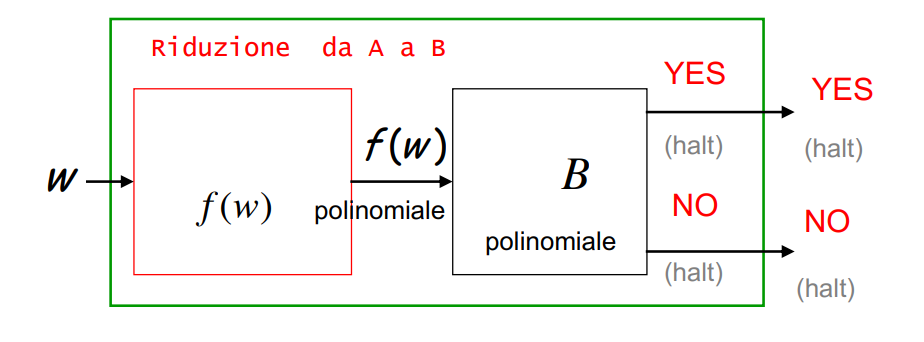
\includegraphics[scale = 0.5]{imm/riduzione.PNG}
    \label{fig:my_label}
\end{figure}
Ad esempio, vertex-cover è NP-difficile, questo significa che posso risolvere ogni problema $A$ in NP con il problema vertex-cover $B$. Per fare questo, si trasforma l’input $w$ di $A$ in un input $f(w)$ per $B$ in tempo polinomiale. La risposta di $B$ con input $f(w)$ è la stessa che $A$ da su input $w$.
\newline
\textbf{UN PROBLEMA NP-DIFFICILE NON è DETTO CHE STIA DENTRO I PROBLEMI DI TIPO NP, NEL CASO IN CUI STIA DENTRO NP ALLORA POSSIAMO DIRE CHE è NP-COMPLETO}

\subsubsection{Riduzione polinomiale da A a B}
Consiste nel trasformare l’input $w$ di $A$ in un input $f(w)$ per $B$ in tempo polinomiale (il calcolo di $f(w)$ è $\mathcal{O} (|w|^p)$). La risposta di $B$ con input $f(w)$  è la stessa che $A$ da su input $w$.
Si ha che $A$ si riduce polinomialmente a $B$, e si scrive: $A\leq_p B$ se $\exists \ f$ tale che: $w \in L_A\mbox{ sse } f(w)\in L_B$ con $f$ calcolabile in tempo polinomiale.

\subsubsection{Definizione di NP-difficile}
Avevamo detto che ogni problema $A$ che in \textbf{NP} può essere risolto con una chiamata di procedura a $B$, quindi posso risolvere ogni problema $A\in NP$ con \textit{vertex-cover}, essendo esso un problema \textbf{NP-difficili}, ma cosa sono i problemi NP-difficili?

Un problema $B$ è NP-difficile se e solo se $\forall \, A \in NP$ , $A$ si riduce a $B$ in tempo polinomiale, cioè $A \leq_p B$.

Un problema $NP-difficili$ può non essere in $NP$, in quanto potrebbe non avere un certificato (y) per consentire la verifica in tempo polinomiale. \\ 
Un problema \textbf{NP-difficili} e anche \textbf{NP} si dice che il problema è \textbf{NP-complete}. Sappiamo inoltre che $SAT$ è il primo problema che si è dimostrato essere anche \textbf{NP-complete}.

Esistono problemi NP-difficili non in NP.

\begin{enumerate}
    \item SAT è il primo problema che si è dimostrato essere NP-completo.
    \item 3-SAT $\leq_p$ IND-SET
    \item IND-SET è NP-completo
\end{enumerate}

$\phi_w$ è soddisfacibile sse $G_\phi$ (che rappresenta $f(w)$) ha un IND-SET di dimensione $k=|\phi| = $ numero di clausole della formula.

Data una istanza $\phi$ di 3-SAT, costruiamo una istanza $(G, k)$ di IND-SET che ha un insieme indipendente di dimensione $k$ sse $\phi$ è soddisfacibile. 
Per farlo si costruisce un grafo $G$ che contiene 3 vertici per ogni clausola, uno per ogni letterale della clausola. In seguito collego i 3 letterali di una clausola con un triangolo (formando un gadget) e si collega ogni letterale al suo negato.
\begin{figure}[H]
    \centering
    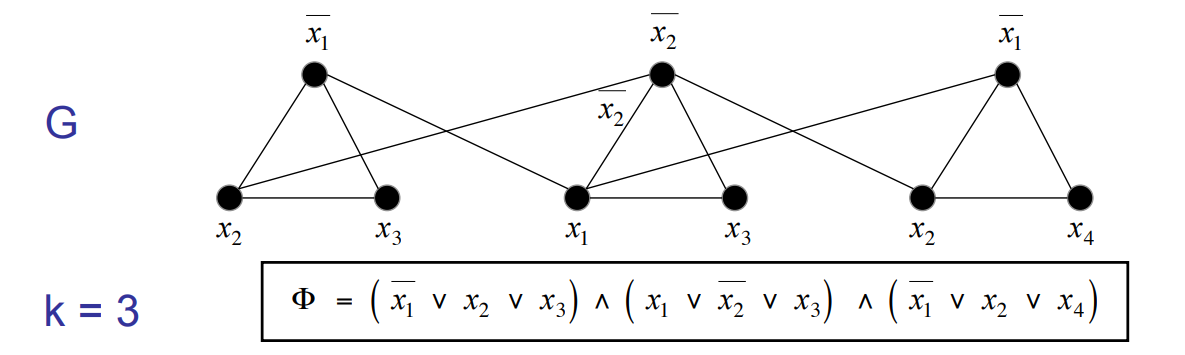
\includegraphics[scale = 0.5]{imm/g-3.PNG}
    \label{fig:my_label2}
\end{figure}
\section{Lezione del 15 ottobre - Bonizzoni}
Un \textbf{gadget} è una rappresentazione dell'input del problema $A$ di partenza e ogni \textbf{gadget} rappresenta una clausola.\\ Ricordiamo che $\phi$ è soddisfacibile sse esiste un assegnamento delle variabili della formula tale per cui almeno un letterale di ogni clausola è vero. \\
Inoltre il concetto di \textbf{riduzione} è quindi ritrovabile nella capacità di rappresentare un problema in un'altra forma, studiabile con un altro algoritmo.
\subsection{Riduzione 3-SAT a INDIPENDENT SET}
Vogliamo dimostrare 3-SAT (A) si riduce polinomialmente a INDIPENDENT SET (B). [3-SAT $\leq_p$ IND-SET] \\

Abbiamo dimostrato l'esistenza della funzione $f$, che trasforma $\phi$ (ovvero l'input di $A$) in $\langle G, k\rangle$, ovvero l'input di $B$, e che essa è in tempo polinomiale. \\
Abbiamo quindi che $w\in L_A$ sse $f(w)\in L_B$. Se $\phi$ è vera allora esiste un \textit{independent-set} di dimensione $k$ per $\langle G, k\rangle$.\\ Nell'altro verso abbiamo che se esiste un \textit{independent-set} di dimensione $k$ per $\langle G, k\rangle$ allora $\phi$ è vera. Dimostrare questi due versi equivale a dimostrare la riduzione.\\

\subsection{Dimostrazione}
\begin{enumerate}
    \item $\exists f$ che trasforma $\phi$ (input di $A$) in $\langle G,k \rangle$ (input di $B$) e $f$ è polinomiale.
    \item  $w \in L_A$ sse $f(w) \in L_B$. Quindi $\phi$ è vera sse esiste un insieme indipendente di dimensione $k$ per $\langle G,k \rangle$.
    
    Se $\phi$ è vera esiste un insieme indipendente di dim $k$ per $\langle G,k \rangle$. Dato un assegnamento di verità, si seleziona un letterale (un vertice) vero da ogni triangolo ottenendo $S$. Questo insieme $S$ è indipendente e di dimensione $k$. \\
    Se $\phi$ è vera, allora $\forall$ clausola $c_i$, $\exists$ letterale $l_{ij}$ che rende vera $c_i$ tale letterale è un vertice del triangolo del gadget $G_{c_{i}}$. Poiché tutte le clausole sono vere, si ha la scelta di $k$ vertici se $k$ sono le clausole. Per cui esiste un insieme indipendente di dimensione $k$.\\
        
    \textbf{\textit{Osservazione}: per definizione se scelgo di rendere vera $c_i$ con $x_j=1$, non posso rendere vera $c_k$ con $\overline{x_j} = 0$.} \\
    \textbf{Dimostrazione per costruzione/assurdo} \\
    
    Se si rende vera la clausola $c_s$ con $l_s$, significa che la variabile $x_i$ è usata o come 1 o come 0 nell’assegnamento di verità in un altro letterale $l_t$ che rende vera la clausola $c_t$. $x_i$ se usata non può essere usata con valore opposto a quello usato per $c_s$. Quindi non esiste un arco di collegamento tra $c_s$ e $c_t$. \\ 
    Si può dimostrare anche per \textbf{assurdo}. Se esiste un arco tra i due letterali $l_s$ e $l_t$ che rendono vere le clausole $c_s$ e $c_t$, allora ottengo una contraddizione sugli assegnamenti di verità, asserendo che i due letterali sono uno la negazione dell'altro ma entrambi sono veri, per poter rendere vere le clausole.\\
    
    Se esiste un insieme indipendente di dimensione $k$ per $\langle G,k \rangle$, allora è possibile trovare un assegnamento alle variabili $\langle x_1, x_2, \dots, x_m \rangle$ che rende vera $\phi$.\\
    Se esiste un insieme indipendente, di dimensione $k$, significa che $\forall$ gadget (clausola) $G_{c_i}$, esiste un vertice nell’insieme indipendente. Quindi esiste un letterale $\forall$ clausola tale che non è collegato ad un altro letterale di un altro gadget. Pertanto, data la clausola $c_s$ esiste un letterale $l_s$ della clausola che non è collegato, in quanto indipendente, a $l_t$ letterale per la clausola $c_t$. \\
        
    Vado $\forall$ letterale $l_i$ c’è una variabile che rende vera $l_i$. Con il valore dato alla variabile, si costruisce l’assegnamento 0/1 a quella variabile, cioè se $l_i=\overline{x_j}$, pongo $x_j = 0$, mentre se $l_i = x_j$ pongo $x_j = 1$. In questo modo si trova un assegnamento di valori alle variabili che è di verità per $\phi$, dimostrando che $\phi$ è vera.
\end{enumerate}

\section{Lezione del 19 - Bonizzoni}
Alcuni fatti:
\begin{itemize}
    \item Se un problema NP-completo è in P (cioè ha un algoritmo polinomiale che lo risolve), allora $P = NP$.
    Per dimostrarlo, per definzione di NP-difficile, sappiamo che per $\forall \ A \in NP,\,\,A \leq_p \Pi$. Ovvero $\Pi$ è una procedura che risolve A, dopo che ho trasformato l'input $x$ di $A$ in input $f(x)$ per $\Pi$, con $f(x)$ calcolabile in tempo polinomiale.\\ Assumendo quindi che $\Pi\in P$ allora anche ogni $A\in P$, e quindi $NP=P$.
    \item La riduzione polinomiale è transitiva. Significa che se $A\leq_p B$ e $B\leq_p C$ allora: $A\leq_p C$. Questa transitività deve necessariamente essere dimostrata. \\ \\
    Infatti $A\leq_p B$ implica l'esistenza di $f$ tale che $x\in L_A$ sse $f(x) \in L_B$. Ugualmente $B\leq_p C$ implica l'esistenza di $g$ tale che $x\in L_B$ sse $g(x) \in L_C$.\\
    L'obiettivo è quello di dimostrare che $\exists \ f'$ tale che $x\in L_A$ sse $f'(x)\in  L_C$. Per formare $f'$ dobbiamo partire da $f$ e $g$ assumendo che $f'() = g \cdot f()$. L'idea di base corrispondere a prendere $x \in L_A$ con $f(x) \in L_B$, se questo è vero possiamo applicare la nostra funzione $g(x)$ potendo quindi eseguire $g(f(x))$. Questo ci permette di dire che $g(f(x))$ appartiene alle istanze di $C$, dimostrando così la transitività. \\
    In altre parole ho che $x \in L_A$ e che $f(x)\in L_B$ (quindi $f(x)$ è un input per $B$) ma quindi $g(f(x))\in L_C$ (quindi $g(f(x))$ è un input per $C$). \\
    Poiché $f$ è calcolabile in tempo polinomiale $|x|$ e anche $g$ è calcolabile in tempo polinomiale in $|f(x)|$, deduco che $f'=g\circ f$ è calcolabile in tempo polinomiale $|x|$. Questo ci consentirà di dimostrare quali problemi entrino nei NP-Completi. \\
    
    Quindi per dimostrare che un problema $\Pi'$ è \textbf{NP-difficile}, devo ridurre $\Pi'$ ad un problema qualsiasi \textbf{NP-difficile} (in base alla somiglianza del problema), sapendo che $\forall A\in NP$ $A$ si riduce ad un problema \textbf{NP-difficile}, come $SAT$.\\ In modo equivalente per dire che è un problema è \textbf{NP-complete} faccio quanto fatto per \textbf{NP-difficile} ma devo aggiungere che esso sia in $NP$, dovendo quindi aggiungere il certificato per dimostrare che la verifica si possa fare in tempo polinomiale.
\end{itemize}

\subsection{Set Cover}
Dato un universo $U$ di $n$ elementi sia $S=\{S_1,\ldots,S_M\}$ una collezione di sottoinsiemi di $U$. Sia anche data una funzione di costo $c:S\to\mathbb{Q}^+$. Il problema \textbf{set-cover} consiste nel trovare una collezione $C$ di sottoinsiemi di $S$ di costo minimo che copra tutti gli elementi di $U$. Se il costo è uniforme, il problema set cover chiede di trovare una sottocollezione che copra tutti gli elementi di $U$ e che abbia minima dimensione.\\

\textit{set-cover}, nella versione decisionale e nella versione con peso uniforme, è \textbf{NP-complete}. Quindi il problema ci chiede se esiste una collezione $C$ di sottoinsiemi di $S$ la cui unione sia $U$ con cardinalità minore uguale di $j$.
\subsubsection{Dimostrare che SC è in NP}
Data una sottocollezione $C$ posso facilmente dimostrare che $|C|\leq k$ in tempo polinomiale e che l'unione degli insieme di $C$ include tutti gli elementi di $U$, in tempo polinomiale su $|U|$. 
Posso aggiungere anche un certificato, nella forma di una collezione che copre tutto $U$ (e quindi la verifica è in tempo polinomiale nell'input e nel certificato). Quindi \textbf{set-cover} è in \textbf{NP}.\\ 

Per dimostrare che \textbf{set-cover} è \textbf{NP-difficile} dimostro che: $\mbox{vertex-cover} \leq_p \mbox{set-cover}$ ovvero uso un problema che so già essere \textbf{NP-difficile}, appunto \textit{vertex-cover}.\\ 

Devo quindi trasformare un'istanza di \textit{vertex-cover} $C=\langle G=(V,E), j\rangle$ in un'istanza $C'$ di \textit{set-cover}, in tempo polinomiale, tale che $C$ è soddisfacibile sse $C'$ è soddisfacibile (se risponde YES su input $C$ e $C'$).\\ 
Eseguo l'assegnamento  $U = E$. Per quanto riguarda la collezione $S$ procedo nel seguente modo. Etichetto i vertici in $V$ da $1$ a $n$. Sia $S_i$ l'insieme degli archi incidenti al vertice $i$-simo.Sia poi $k=j$ per concludere la costruzione polinomiale dell'istanza di \textit{set-cover}.\\ Ciascun arco è un elemento di $U$ e ciascun vertice è un insieme di $S$.\\

Vediamo anche la dimostrazione formale che \textit{vertex-cover} risponde yes, per $j$, sse istanza di \textit{set-cover} risponde yes per $k=j$.\\ Innanzitutto se \textit{vertex-cover} risponde yes per $j$ allora trovo una collezione di \textit{set-cover} buona di cardinalità $j$. 

supponiamo che $G$ ha una copertura C di al più $j$ vertici. Per costruzione, $C$ corrisponde ad una collezione $C'$ di sottoinsiemi di $U$. Poiché assumo $k=j$ allora $|C'|\leq k$. Inoltre $C'$ copre tutti gli elementi di $U$ poiché $C$ copre tutti gli archi di $G$. Per mostrare questo prendo ogni elemento di $U$ che è un arco in $G$. Poiché $C$ è una copertura,
almeno un estremo dell'arco è in $C$ e quindi l'arco è in un insieme di $C'$. Dimostriamo anche l'altro verso della dimostrazione, ovvero devo garantire l'esistenza della copertura. \\
Suppongo di avere un set cover $C'$ di dimensione al più $k$ nella nostra istanza. Dato che ad ogni insieme di $C'$ ho associato un vertice in $G$,  sia C l’insieme di quei vertici, allora $|C|=|C'|\leq k=j$. Inoltre, $C$ è una copertura di $G$ poiché $C'$ è un set-cover, poiché, preso un arco $e$ ho che $e\in U$ e quindi $C'$ deve contenere almeno un insieme che include $e$ e tale insieme è quello che corrisponde ai nodi che sono estremi di $e$. Quindi $C$ deve contenere almeno un estremo di $e$. Quindi posso concludere dicendo che $C$ è copertura di $G$.
\section{Lezione del 20 ottobre - Bonizzoni}

Si continua la ricerca di una dimostrazioni di \textbf{NP-completezza}, ambito di studio nato dopo la scoperta di Cook che dimostrava $SAT\in$ \textbf{NP-complete}.\\ 
Ricordiamo:
\begin{itemize}
    \item Se $B$ è un problema tale che $A\leq_p B$, con $A$ \textbf{NP-hard} (o ovviamente anche \textbf{NP-complete}), allora $B$ è \textbf{NP-hard} e se inoltre $B\in NP$ allora $B$ è \textbf{NP-complete}.
    \item Con la transitività della riduzione $\leq_p$ si ha che $\forall\Pi\in NP, \quad \Pi\leq_p A$ e quindi $A$ è \textbf{NP-hard}. Inoltre avendo $A\leq_p B$ ho che  $\Pi\leq_p B$ e quindi $B$ è \textbf{NP-hard}, inoltre, avendo $B\in NP$, ho che è \textbf{NP-complete} 
\end{itemize}   

\subsection{Clique Problem}

Definisco \textbf{clique} (cricca) di un grafo non orientato $G=(V,E)$ come un sottoinsieme $V'\subseteq V$ di vertici tale che: $\forall \,v_1,v_2\in V' (v_1,v_2)\in E$ quindi un sottoinsieme di vertici con solo vertici collegati da un arco.\\
Il \textbf{clique-problem} è un problema di ottimizzazione (nel dettaglio di massimo) in cui si cerca la \textbf{clique} di dimensione massima di un grafo (ovvero $|V'|$ è massimo). Nella versione decisionale chiedo se esiste una \textbf{clique} di dimensione $k$.\\ Il problema \textit{clique} è \textbf{NP-complete}.

\subsubsection{Dimostrazione clique in NP}
Per dimostrare che la \textit{clique} $\in $ NP, per un grafo $G=(V,E)$, usiamo un insieme $V'$ di vertici nella cricca come certificato per l'input $G$. Per verificare che $V'$ è una cricca (dove $V'$ avrà la dimensione pari alla domanda di decisione, ovvero $|V'| = k$) controllerò che $\forall u,v \in V'$, $(u,v) \in E$. Tale verifica è in tempo polinomiale, corrisponde infatti a $\mathcal{O}(|V'| \cdot |V'|)$, ed è quindi quadratico nella dimensione dell'input.

Bisogna ora trovare un problema $A\in {NP-complete}$ tale che $A$ si riduce, in tempo polinomiale, al \textbf{clique-problem} (quindi \textbf{clique-problem} risolve $A$). \\ 
Notiamo che una clique è l'opposto di \textbf{independent-set}, che avevamo dimostrato tramite $3SAT$ (che può risolvere \textbf{independent-set}).\\ 
Quindi per \textbf{clique-problem} provo ancora ad usare $3SAT$. Devo fare in modo che $\phi\in 3SAT$ sse il grafo $G_\phi =(V,E)$ ha una clique di dimensione uguale al numero di clausole di $\phi$. Quindi avendo $k$ clausole in $\phi$ avrò che ciascuna clausola sarà un gadget e da ogni gadget viene preso un singolo vertice che comporrà la clique di dimensione $k$.\\    
Il grafo $G_\phi$ è costruito come nel caso di \textit{independent-set} coi letterali come vertici.\\ Bisogna studiare il collegamento tra tali vertici (che sarà diverso al caso di \textit{independent-set}, non avendo quindi i triangoli).\\

Ipotizzo: 
$\phi=c_1\land c_2\land c_3$ con: $c_1=x_1\lor \neg x_2\lor \neg x_3$, $c_2=\neg x_1\lor x_2\lor x_3$, $c_3=x_1\lor x_2\lor x_3$. \\ 
Per ogni clausola faccio i vertici per ogni letterale (distinti anche per lo stesso letterale, come nel caso di \textit{independent-set}).\\ 
Collego ogni letterale di ogni clausola con ogni altro letterale di ogni altra clausola (non della stessa) a patto che non siano il loro negato, collegando quindi solo vertici \textbf{consistenti}.
\begin{figure}[H]
    \centering
    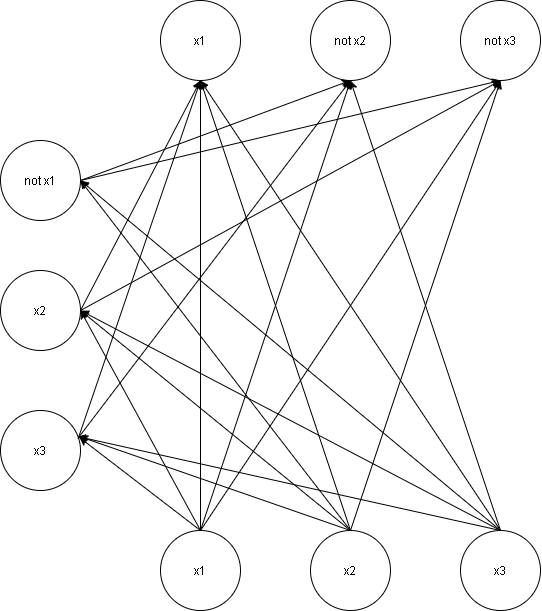
\includegraphics[scale = 0.3]{imm/grafico.png}
\end{figure}

La regola per trasformare $\phi$ nel grafo $G_\phi$, già descritta sopra, la scriviamo ora in modo formale:
\begin{itemize}
    \item per ogni clausola $\displaystyle \in \phi$, $c_r = (l_1^r \lor l_2^r \lor l_3^r $, definiamo un gadget che è un grafo ($G_{c_r}$) che consiste di 3 vertici: $\displaystyle v_1^r \lor v_2^r \lor v_3^r$ in $V$. Dove $\displaystyle V = \bigcup \{v_1^i \lor v_2^i \lor v_3^i\}$, dove però $1 \leq i \leq k$.
    \item $\forall \  v_i^s \lor v_j^r \ \exists $ l'arco $\in E$, sse $l_i^s \lor l_j^r$ sono \textit{consistenti} (il letterale $l_i^s$ non è la negazione di $l_j^r$)
\end{itemize}
Non potrò mai avere più di un letterale per clausola nella clique non essendo tra loro collegati.\\ Passare da $\phi$ a $G_\phi$ ha costo polinomiale in tempo, ottenendo quindi istanza, in tempo polinomiale. \\

Bisogna dimostrare che se $\phi$ ha un assegnamento che la rende vera allora esiste una clique per $G_\phi$ di dimensione $k$. 
Se $\phi$ è vera allora per ogni clausola $c_r$ esiste almeno un letterale che è vero, e assumiamo che tale letterale sia $l_{i}^r = 1$. 
Questo letterale è associato al vertice $v_i^r$ del grafo.Quello che dobbiamo fare è costruire l'insieme dei vertici $V'\subseteq V$ tale che sia formato da quei singoli vertici, $V' = \{ v_i^1, v_j^2 \dots v_z^k\}$, corrispondenti ai singoli letterali veri.  \\ 
L'insieme $V'$ enunciato è una clique, infatti avrò solo letterali collegabili nel grafo, per dimostrarlo dico che $\forall u,v \in V'$, $(u,v) \in E$, ovvero ho solo archi tra letterali consistenti tra loro e quindi, per costruzione, esiste l'arco tra i vertici corrispondenti ($\forall\, u,v\in V'$).\\ 

Inoltre bisogna dimostrare che, se esiste una clique di dimensione $k$, allora $\phi$ è vera e quindi le $K$ clausole sono tutte vere. \\ Per ogni vertice di $v_{it}\in V'$ se appartiene al gadget della clausola $c_t$ rendo vero il letterale associato (o falso se esso è negato). A questo punto rendo vera ogni clausola rendendo vero il letterale associato al vertice della clausola. Da questo so di ottenere un assegnamento di verità per $\phi$ in quanto i letterali sono consistenti. 
\section{Lezione del 27 ottobre}
Riprendiamo il discorso in cui affermiamo che Clique è in \textbf{NP} e in \textbf{NP-difficile} di cui è stata dimostrazione.

Quello che vogliamo vedere oggi è che la trasformazione di una formula $\phi$, dopo aver fatto la riduzione da 3Sat a Clique, in un grafo $G$ è una riduzione.
\subsection{Dimostrazione}
Per la dimostrazione si devono dimostrare le due direzioni:
\begin{enumerate}
\itemsep1pt\parskip0pt\parsep0pt
    \item \textbf{Dato un assegnamento di verità della formula, si costruisce la clique} Dato un assegnamento che rende vera la formula $\phi$ (che ha $k$ clausole), bisogna costruire una clique per il grafo $G$ che abbia $k$ vertici.\\ Ciascuna clausola $c_r$ ha almeno un letterale $l_i^r$ che ha valore assegnato pari a $1$. Ciascun letterale corrisponde ad un vertice $v_i^r$ (si ha che $l_i^r \to v_i^r$). Si costruisce l'insieme $V'$ di vertici per ogni letterale $l_i^r$ vero (e quindi per ogni clausola $c_r$). Si dimostra che $V'$ è una clique. \\ Infatti per ogni coppia $v_i^r, v_j^s \in V'$ con $r \neq s$, abbiamo che $(v_i^r, v_j^s) \in E$ e entrambi i letterali sono consistenti, ovvero uno non è derivato dalla negazione di una variabile presa come positiva nell'altro letterale.
    \item \textbf{Data una clique, si costruisce l'assegnamento di verità della formula} Si supponga che $G$ abbia una clique $V'$ di dimensione $k$; bisogna quindi far vedere che $\phi$ è vera.\\ Per costruzione $V'$ ha esattamente un solo vertice per ogni clausola ($v_i^r$ per la clausola $c_r$). Quindi per ogni clausola $c_r$ si assegna al letterale corrispondente $l_i^r$ il valore $1$. Sapendo che il letterale complementare $l_i^r$ non verrà usato per rendere vera una clausola in quanto il vertice $v_i^r$ non è collegato con un arco ad un vertice che rappresenta il complemento di $l_i^r$. Quindi si riesce a costruire un'assegnamento di verità consistente per $\phi$, ovvero ogni variabile viene presa come $x_i = 0$ oppure come $x_i = 1$, non utilizzando mai entrambi i valori.
\end{enumerate}
La struttura dimostrativa è sempre la stessa, si hanno infatti due direzioni ogni volta, quindi sarà sempre una situazione dove $\displaystyle x_{\in I_A} \to f_{\in I_B}(x)$ con riduzione polinomiale messa nel modo $A \leq_p B$. Ora ci serve mostrare che se x appartiene al linguaggio A (cioè ammette risposta affermativa) allora f(x) appartiene al linguaggio di B. Lo possiamo scrivere come $x \in L_A \to f(x) \in L_B$.

Si può fare la dimostrazione che Clique $\leq_p$ Vertex Cover, avendo visto un esempio simile Independent set $\leq_p$ Vertex Cover (e viceversa). \hfill

Possiamo osservare che se $A \leq_p B$ e $A, B \in$ NP-completi $\to B \leq_p A$.\hfill
\subsection{Problemi di ottimizzazione}
Dato un problema $\Pi$ e un'istanza $x$, l'ottimo su $x$ di $\Pi$, indicato come $opt()$, è il valore numerico che quantifica la soluzione ottimale (tra tutte quelle ammissibili), ovvero quella che massimizza o minimizza una certa funzione costo. Il costo di una soluzione ammissibile su $x$ calcolato da un algoritmo $A$ per il problema $\Pi$ viene indicato con $A(x)$. Tra tutte le soluzioni ammissibili di $\Pi$, sicerca la soluzione che massimizza o minimizza un costo. 

\textbf{Algoritmo $\varepsilon$-approssimato} per un problema $\Pi$ di ottimizzazione è un algoritmo $A$ polinomiale tale che restituisce una soluzione ammissibile che dista da quella ottima di un fattore costante $\varepsilon$. 
\begin{itemize}
    \item Se $\Pi$ è un problema di minimo allora: $A(x) \leq \varepsilon \cdot opt(x)$ dove $\varepsilon > 1$.
    \item Se $\Pi$ è un problema di massimo allora: $A(x) \geq \varepsilon \cdot opt(x)$ dove $0 < \varepsilon < 1$, in questo caso notiamo che il valore di $\varepsilon$ viene dato per mezzo di una frazione.
\end{itemize}
La caratteristica della $\varepsilon - approssimazione$ è che vado a trovare un $A$ che lavora in tempo polinomiale che risolve in modo approssimato un problema tendenzialmente in NP-completo. \\
Il fattore $\varepsilon$, che è una costante numerica che non dipende dall'input, funge da \textbf{garanzia} sulla distanza dal costo della soluzione trovata da quella ottimale. Ricordiamo che $A(x)$ è il costo della soluzione ammissibile calcolata da un algoritmo A.

Quando si parla \textbf{tasso di approssimazione (approximation ratio)} ci sono diverse approssimazioni. Quello che però identifica sono le prestazioni di un algoritmo di approssimazione possono essere valutate mediante: 
\[
    \max
    \begin{Bmatrix}
    \displaystyle \frac{A(x)}{opt(x)}, \frac{opt(x)}{A(x)}
    \end{Bmatrix}
    \leq r
\]
Dove
\begin{itemize}
    \itemsep1pt\parskip0pt\parsep0pt
    \item $A(x)$: soluzione approssimata
    \item $opt(x)$: soluzione ottima
    \item $r$: fattore di approssimazione (utilizzato al posto di $\varepsilon$ al fine di avere sempre un valore intero).
\end{itemize}

Non tutti i problemi NP-completi ammettono una $r$-approssimazione, per $r$ costante. Infatti il tasso di approssimazione può essere espresso mediante una funziona $\rho(n)$ che dipende dalla dimensione dell'input ($|x| = n$). La dimensione del problema influisce sulla capacità di approssimare il problema, in poche parole l'approssimazione peggiora all'aumentare delle dimensioni del problema.

\begin{figure}[H]
    \centering
    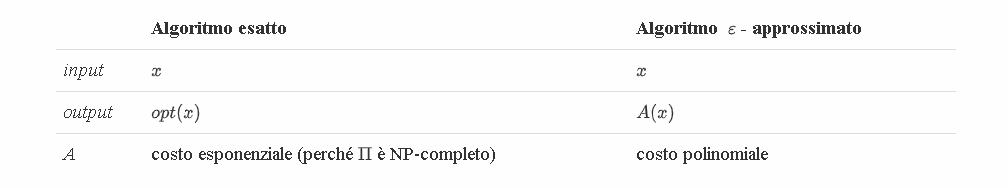
\includegraphics[scale = 0.5]{imm/algoritmo_esatto.PNG}
\end{figure}

$\exists$ un algoritmo $A$ polinomiale per Vertex Cover 2-approssimante trovandomi ad affrontare $\displaystyle \frac{A(x)}{opt(x)}\leq 2$.
Per trovare $\varepsilon$, si fornisce un'euristica $A$ per Vertex Cover, cioè un modo per ottenere in tempo polinomiale una copertura di vertici per $G$, e poi si prova a dimostrare, senza conoscere $opt(x)$ (per ogni input $x$), che $\displaystyle \frac{A(x)}{opt(x)} \leq \varepsilon$ e si ha una $\varepsilon$-approssimazione.\\
Pur non conoscendo l'ottimo è possibile fare una stima del valore del rapporto, perché è possibile immaginare come potrebbe essere l'ottimo in funzione dell'input.\\

\subsection{Vertex Cover Approx}
Inventare un'euristica polinomiale per calcolare una copertura per un grafo (Vertex Cover) con $G = (V. E)$. 
Cerco un $A$ che calcoli in tempo polinomiale una soluzione ammissibile, ovvero una copertura di vertici del grafo. Si sceglie che $A$ non deve essere un \textit{algoritmo greedy}. Prendo quindi un arco del grafo $e=(u,v)\in E$. Inizio a costruire una copertura $C$, all'inizio vuota ($C=\emptyset$), che ora diventa, aggiungendo i due vertici: $C=C\cup\{u,v\}$\\
Inoltre rimuovo dall'insieme degli archi $E$ tutti gli archi che hanno un estremo nell'attuale copertura $C$, e quindi nel nostro caso in $u$ o $v$. La copertura $C = \varnothing$, risulta la mia soluzione ammissibile che inizialmente la troviamo vuota. Finché $E = \varnothing$.
L'algoritmo restituisce: $A(x) = 2 \times $numero di archi scelti in $E$.

\begin{lstlisting}
Approx(G)
C  := null 
E' := archi di G
while E' != null do 
    let (u,v) appartenente a E'
    C := C union {u,v}
    per ogni (u,z) in E', (v,z') in E'
        rimuovi (u,z), (v,z') da E' 
return C
\end{lstlisting}

È un algoritmo polinomiale nella dimensione di $G$ ($|V|, |E|$).

È quindi una 2-approssimazione in quanto al massimo posso prendere il doppio dei vertici per fare la copertura, infatti, per costruzione, seleziono ogni volta archi che non hanno estremi in comune. Per ognuno di questi archi scelti devo prendere i due estremi, quindi ho $2\cdot k$ vertici in $C$ per $k$ archi e quindi: $A(x)=2\cdot k$.
Ma di $opt(x)$ so che nel casi migliore prende esattamente un estremo per ogni scelto dall'algoritmo, e quindi per archi che non hanno estremi in comune. Quindi nel caso migliore: $opt(x)\geq k$. Ma dato che stiamo cercando di minimizzare, quindi $k$ è il \textit{lower bound} vale quindi: $\displaystyle\frac{A(x)}{opt(x)}\leq\frac{2k}{k}\leq 2$.
\section{Lezione del 3 novembre}
L’algoritmo per Vertex Cover-Approx, nel nostro caso lo chiamiamo $opt(x)$, nel caso migliore prende esattamente un estremo per ogni arco scelto di volta in volta da A.
$$A(x) = 2k (\mbox{ con } 2k \mbox{ vertici in } C)$$
$k$: numero di archi, che pone un limite inferiore alla dimensione dell’ottimo ($opt(x) \geq k$).
$\displaystyle \frac{A(x)}{opt(x)} \leq \frac{2k}{k} \leq 2$

L’idea della 2-approssimazione è quella che:
\begin{itemize}
    \item si cerca un limite inferiore $k$ alla dimensione dell’ottimo per il problema su istanza $x$: $opt(x) \geq k$. Ricordiamo che $x$ è una istanza del grafico $G = (V,E)$
    \item si sviluppa un algoritmo polinomiale $A(x)$ che produce una soluzione ammissibile per il problema tale che il costo di tale soluzione sia $\varepsilon \cdot k$, per $\varepsilon > 1$. Indichiamo come $A(x)$ la dimensione di un matching.
    \item Dal momento che $opt(x) \geq k$ e $A(x) \leq \varepsilon \cdot k$, con $\varepsilon > 1$, allora $\displaystyle \frac{A(x)}{opt(x)} \leq \frac{\varepsilon \cdot k}{k} \leq \varepsilon$.
\end{itemize}
Quindi diciamo che nel caso del Vertex-Cover, dato che $x$, ricordiamo sia una istanza del grafo, allora $A(x)$ è la dimensione di un matching. Si costruisce quindi un matching perfetto, selezionando degli archi del grafo che non condividono i vertici o estremi. Si cerca di utilizzare tutti i vertici.\\

Una copertura minima del grafo deve per forza contenere esattamente un vertice per ogni arco del matching (perché non hanno estremi in comune). Quindi il limite inferiore per $opt(x)$ è il numero di archi del matching. Questo posso indicarlo con $opt(x) \geq$ numero di archi del matching.\\
L’algoritmo $A$ costruisce in maniera incrementale (un simil greedy) un matching per $G$ come segue: prende un arco $e_i$ e rimuove tutti gli archi incidenti agli estremi di $e_i$.Per fare questo, però inserisce nella soluzione ammissibile i due estremi di $e_i$. L’arco successivo scelto da $A$ non ha estremi condivisi con $e_i$. \\ In sintesi l'unico problema è che la dimensione di $A(x)$ è doppia rispetto al numero di archi del matching (perché salvo tutti i vertici): $A(x) = 2 \times$ numero di archi nel matching, mentre $opt(x) \geq$ numero di archi del matching, perché non è detto che per l'ottimo bastino il numero di archi del matching.

{
\paragraph{Domanda e-mail}

Esistono dei problemi NP-hard per i quali non si è riusciti a dimostrare che stiano anche in NP, ovvero per i quali non si è riusciti a costruire un algoritmo con certificato.
}\\

Un problema $\Pi$ è completo per una classe di complessità $K \iff$ il problema $\Pi$ è nella classe stessa, quindi $K$ ed è difficile per la classe $K$.  
\subsection{Complessità parametrica}
Dato un problema NP-completo, questo può avere istanze che sono risolvibili in tempo ragionevole se si fissano dei parametri che caratterizzano l’istanza. Se il parametro è piccolo anche un tempo esponenziale in $k$ è accettabile.

Esempio: dato un grafo, esiste un vertex-cover di dimensione al più $k$?

Un problema decidibile $\Pi$ è trattabile fissato il parametro (FTP, Fixed Parameter Tractable) $k \iff \exists$ un algoritmo $A$, una costante $c$ e una funzione computabile $f$ tale che $\forall$ input $\langle x, k \rangle$, $A$ risolve il problema con tempo di calcolo $f(k)|x|^c$. \\

Notiamo che $|x|^c$, ovvero la parte relativa all'input, è un tempo polinomiale, mentre $f(k)$ è un tempo esponenziale.
Vediamo quindi il tempo $T(n)$ come funzione di $n =|x|$ e di $k$. Deve valere che $k$ è piccolo, essendo esponenziale si accettano valori piccoli. \\

Se mi trovo in un problema di decisione, quindi con un $bound$ imposto, che noi denominiamo $k$, significa che non ho più il problema generale dell'ottimizzazione (quello che abbiamo visto $opt()$), prendo in considerazione una versione ristretta del problema di decisione, questo per via di $k$ che avevamo voler tenere di piccole dimensioni per non avere tempi di calcolo troppo alti. Si crea quindi un algoritmo parametrico che utilizza $k$, tale per cui il tempo di calcolo risulta essere una funzione  $f(k)n^c$, dove $n$ è il massimo della cardinalità dei vertici definiti $e_i$ prima. \\


\subsection{Alberi di ricerca limitati}
Dato che possiamo fissare il tempo imposto un valore di bound $k$ grazie al passaggio di un valore, espresso come parametro , al nostro algoritmo, possiamo costruire algoritmi parametrici.\\
Solitamente gli algoritmi parametrici, o qualsiasi tecnica parametrica, utilizzano gli alberi di ricerca limitati. 

\begin{teorema}{Teorema}{}
    Il problema vertex-cover $(G,k)$ è risolvibile in tempo $\mathcal{O}(2^k |V|)$, dove V è l'insieme dei vertici di di G. La costante rappresentata dal nostro $\mathcal{O}$ non dipende da $k$ e nemmeno da $V$. Quella è semplicemente la funzione che esprime il tempo di calcolo.
    $$\mathcal{O^*}(f(k)) = \mathcal{O}(2^k |V|)$$
\end{teorema}

L'idea, per riuscire a rappresentare un insieme grande di vertici, è quella di costruire i sotto insieme di un numero $k$ di vertici. Questi sottoinsieme sono in totale $2^k$ quando si raggiunge la profondità $k$ passato come parametro.
\section{Lezione del 19 novembre}
\subsection{FPT (Fixed Parameter Tractability)}

Un algoritmo FPT con parametro $k$ fissato e input di dimensione $n$ è un algoritmo con complessità $\mathcal{O}(f(k) \times poly(n))$ in tempo, dove $f(k)$ non dipende da $n$ e non è polinomiale in $n$ (altrimenti il problema sarebbe in P, mentre l’algoritmo si applica a problemi NP-difficili: è un problema di ottimizzazione difficile). \\
Sono solitamente rappresentati da funzioni esponenziali in $k$. Andiamo a considerare $2^k \cdot n$ per certi $k$ e $n$. Il tipo di complessità può portrare la funzione a non essere un semplice $k$, infatti in questo caso abbiamo $2^k$. Andiamo a osservare per quali valori di $k$ la funzione che ha come valore $2^k \cdot n$ sia meglio di $2^n$. Valutando NP-difficili si richiedono tempi esponenziali. I vantaggi rispetto a un tempo $2^n$ si hanno con $k$ non troppo grande.\\

Un algoritmo FPT è ottenibile con diverse strategie, la più comune delle quali è *Bounded Search Tree*.

\textbf{Algoritmo con bounded search tree per Vertex cover}
Per costruire un algoritmo di costo $\mathcal{O}(2^k \cdot |V|)$ per risolvere Vertex Cover di decisione con copertura di dimensione $k$.

L'idea principale che si utilizza in questo caso per coprire gli archi di un grafo $G=(V,E)$ si divide in alcuni step:
\begin{enumerate}
    \item si prende un arco a caso $(u,v)$ tale che un estremo dell’arco ($u$ o $v$) sia nella copertura del grafo.
    \item si provano entrambi gli estremi e si effettua una ricorsione.\textbf{}
\end{enumerate}
Nel caso in cui il problema da risolvere fosse di natura decisionale, quindi un \textbf{Vertex Cover versione di decisione}, avendo come input un grafo $G=(V,E)$ e un intero $k \geq 0$ e si ha come obiettivo quello di stabilire se $G$ ha un vertex cover di dimensione al più $k$, questo rappresenta il nostro output. 
Denominiamo il nostro algoritmo scritto il pseudo codice:
\begin{lstlisting}
    Procedura BoundedSearch(G,k)
    //casi base
    if G = insiemeVuoto then    //corrisponde all'aver considerato tutti gli archi
    	return true
    if k = 0 then               // ogni chiamata riduce k, il grafo non risulta vuoto
    	return false            //esistono ancora archi ma siamo andati oltre k per la copertura
    //ricorsione
    prendi un arco (u,v) di G
    if BoundedSearch(G-u, k-1) then 
    	return true
    if BoundedSearch(G-v, k-1) then
    	return true
    return false 
    /**rappresentazione come albero binario, questo per via di come sono state impostate le chiamate ricorsive*/
\end{lstlisting}
Si nota facilmente che viene effettivamente costruito l'insieme copertura, ma viene riportata solamente il valore booleano in base al fatto se quella copertura esiste.\\
Dall'algoritmo possiamo ricavare che si sta lavorando su un grafo $G$, dove se da queto ultimo viene rimosso  l’estremo $x$: \[G-x = (V-x, E - {\text{archi incidenti a } x})\]
Costo complessivo: $2^k \cdot |V|$.

La ricorsione corrisponde alla creazione di un albero limitato di ricerca. Si parte dalla radice $r$ (in cui si ha tutto $G$ e $k$ come parametro per la ricerca). In seguito si sceglie a caso l’arco $(u,v)$ e si creano due figli (uno per $u$ e uno per $v$ usati per la chiamata ricorsiva), decrementando $k$ di $1$ per scendere in profondità. Questo procedimento si ripete ricorsivamente per i due figli. \\

Al passo ricorsivo generico, per ogni nodo da sviluppare si procede come segue: 
\begin{itemize}
    \item Se un nodo è etichettato dall’insieme $\{X\}$ di vertici, è perché si sta rappresentando il grafo $G-X$ e il parametro $k'$ è dato $k’ = k-|X|$. 
    \item Si sceglie  l’arco $(z,w)$, questo è il passo che precede le due chiamate ricorsive, e si creano due figli per il nodo: $\{X\} \cup z$ e $\{X\} \cup w$, con il decremento di $k'$ che ora è $k'-1$.
    \item Si ripete finché: 
        \begin{itemize}
            \item $G=\emptyset$, quindi sono finiti gli archi e si restituisce `true` perché è stata trovata la copertura. 
            \item $k=0$ (e $G \neq \emptyset$), quindi sono rimasti archi non coperti e si è a profondità $k$, pertanto si restituisce `fail`.
        \end{itemize}
        Alla fine si avranno nodi `true` e nodi `fail`. 
\end{itemize}
Versione che ricostruisce l’insieme vertex cover (minimo) di dimensione $k\leq 2$.

\begin{lstlisting}
    Procedure Vertex-CoverFPT(G,k)
    if G = insiemeVuoto 
    	return insiemeVuoto
    if k = 0
    	return FAIL
    Take (u,v), edge of G
    C1 = {u} || Vertex-CoverFPT(G-u, k-1)
    C2 = {v} || Vertex-CoverFPT(G-v, k-1)
    return min{C1, C2}
\end{lstlisting}

Si consideri lo stesso algoritmo applicato a $G$ con $k=3$. Si scende di $3$ livelli e si ritorna il minimo insieme calcolato dai nodi che non restituiscono `fail`.

Il tempo di calcolo è determinato dal numero di nodi dell'albero di ricorsione limitato (\textbf{bounded search tree}). Si ha che in totale abbiamo $\mathcal{O}(2^k)$ nodi alla profondità $k$ e che per ogni nodo si considera il costo di analisi del nodo. Il costo dell'analisi è pari a:
\begin{itemize}
    \item numero di archi $\mathcal{O}(|E|)$ se si analizzano tutti gli archi incidenti al nuovo estremo $u$ aggiungo al nodo
    \item numero di vertici  $\mathcal{O}(|V|)$ se si considerano i vertici raggiungibili da $u$. 
\end{itemize}
Pertanto il costo in tempo, valutando quindi il caso peggiore, è $\mathcal{O}(2^k \cdot |V|)$
\subsection{Problema del commesso viaggiatore (Traveling Salesman Problem, TSP)}

Bisogna visitare una serie di clienti e tornare al punto di partenza senza tornare due volte dallo stesso cliente seguendo il percorso meno costoso. Molti altri problemi pratici hanno questa struttura. Abbiamo inoltre un costo per ogni possibile collegamento e il costo del percorso è la somma dei costi dei collegamenti percorsi.\\
Quello che sappiamo è che TSP è un problema che rientra nell'insieme NP-completo.\\
Altri problemi che presentano una simile impostazione sono elencati di seguito.
\subsubsection{Ciclo di Eulero}
Si tratta di un ciclo che visita tutti gli archi del grafo una sola volta. È quindi possibile tornare eventualmente nello stesso vertice.

Possiamo discutere anche dei cicli euleriani in maniera più ampia. Questi ci dicono che dato un (multi)grafo non orientato, si definisce\textbf{ ciclo euleriano }un cammino chiuso che passa esattamente una volta per ogni arco. Dove un multigrafo è un grafo in cui esiste almeno una coppia di vertici collegata da più di un arco.
\begin{teorema}{Teorema di Eulero}{}
    Un (multi)grafo ammette un ciclo euleriano $\iff$ il grafo è connesso e ogni nodo ha grado pari (grafo euleriano).
\end{teorema}

Un nodo è di \textbf{grado pari} se il numero di archi entranti corrisponde al numero di archi uscenti.

\subsection{Ciclo Hamiltoniano di peso minimo}
Per modellarlo, si considera un grafo $G(V,E)$ completo, con costi sugli archi $c \in \mathbb{R}^E$. Un ciclo hamiltoniano è un ciclo semplice, non orientato, che passa per ogni nodo di $G$. Il costo del ciclo è pari alla somma dei costi dei suoi archi.\\
Definiamo ciclo semplice come il ciclo in cui non viene ripetuto lo stesso vertice più volte.\\

Il problema del commesso viaggiatore (TSP) consiste nel trovare un ciclo hamiltoniano di costo minimo. Se il grafo non è orientato, si parla di TSP simmetrico; se invece il grafo è orientato si parla di TSP asimmetrico.\\

Il problema appartiene alla classe di problemi combinatori con funzione obiettivo lineare e alla classe dei problemi difficili (NP-hard).

\subsubsection{TSP metrico}
Dato un grafo $G(V,E)$ non orientato, completo con costi $c$ associati agli archi, se 
\begin{itemize}
    \item $c_{(u,v)} \geq 0$, $\forall$ arco $(u,v) \in E$	e	$c_{(u,v)} = 0 \iff u=v$
    \item $c$ è tale che $\forall$ tripla di nodi distinti $(u,v,z)$ si ha che $c_{(u,v)} \leq c_{(u,z)} + c_{(z,v)}$ (disuguaglianza triangolare)
\end{itemize}
allora $c$ induce una semimetrica.


\section{Lezione del 23 novembre}
Esiste un algoritmo polinomiale per costruire un ciclo Euleriano da un grafo Euleriano.\\
Un algoritmo 2-approssimante per il TSP metrico è noto come algoritmo di Christofides.

\subsection{Algoritmo di Christofides}
Dato un grafo $G(V,E)$ non orientato, completo, con costi $c$ semimetrica, l’algoritmo trova un ciclo hamiltoniano di costo al più doppio rispetto al ciclo di costo minimo.
\begin{enumerate}
    \item Si trova il minimo albero ricoprente $T$ di $G$.\\
    L’algoritmo greedy (*algoritmo di PRIN*) garantisce l’ottimo: basta scegliere gli archi in ordine di costo crescente ma saltando quelli che chiudono i cicli.
    \item Si raddoppia ogni arco di $T$ ottenendo un grafo euleriano.
    \item Si costruisce un ciclo euleriano $\mathcal{E}$ di questo grafo (in tempo polinomiale).
    \item Si sceglie un nodo iniziale $u \in \mathcal{E}$ e si visira $\mathcal{E}$ a partire da $u$.
    \item Si costruisce una permutazione $\pi$ dei nodi $V$, sequenziando i nodi nell’ordine della loro prima apparizione in $\mathcal{E}$ nella visita.
    \item Si restituisce il ciclo hamiltoniano $H$ associato a $\pi$. 
\end{enumerate}
$H$ è ottenuto da $\mathcal{E}$, sostituendo cammini con archi: $c(H) \leq c(\mathcal{E})$ per disuguaglianza triangolare.
Evidenziamo una differenziazione della notazione, chiameremo $H^*$ un ciclo hamiltoniano ottimo (con costo minimo), con $H$ invece si indica la soluzione che approssima quella di minimo costo.

Il costo, per costruire un ciclo di Eulero $\mathcal{E}$, è in relazione con il costo dell'albero di copertura minimo $c(T)$, sono nella relazione $c(\mathcal{E}) = 2 \cdot c(T)$. Questo perché $E$ è il ciclo di Eulero del grafo ottenuto duplicando gli archi di $T$ e $E$ attraversa una sola volta tutti e soli gli archi di tale grafo. Questo perché stiamo generando un multi grafo. \\
Si ha che $c(\mathcal{E}) = 2 \cdot c(T)$ perché $\mathcal{E}$ è il ciclo di Eulero del grafo ($G_T$) ottenuto duplicando gli archi di $T$ ed $E$ attraversa una sola volta tutti e soli gli archi di tale grafo($G_T$).  Da questo quindi deriva che \[c(\mathcal{E}) = c(E(G_{\pi})) = 2 \cdot c(T)\]
Quello che ci manca ora per poterci collegare ad $H^*$, date tutte le nozioni apprese fin ora, è esprimere la relazione tra il cammino di costo minimo $c(T)$ e il camino hamiltoniano $H^*$. La relazione che sussiste è data da \[c(T) \leq c(H^*)\]	

Un ciclo hamiltoninao ottimale è costituito da un albero di copertura $T' \ +$ un arco $e$ che chiude l'albero ad un ciclo, per cui  $c(H^*) \geq c(T')$ perché $c(H^*) = c(T') + c(e)$.
$T'$ non è detto che sia l'albero di copertura minima per cui $c(T) \leq c(T')$ dove $T$ invece è l'albero di copertura minimo. Unendo le due relaziono otteniamo che: $c(H^*) \geq c(T') \geq c(T)$.
Possiamo ottenere la seguente rappresentazione 
\[c(T) \leq c(T') \leq c(H^*)\]
\[\Downarrow\]
\[c(T) \leq c(H^*)\]
Da quanto espresso deriva che 
\begin{itemize}
    \item $c(H) \leq c(\mathcal{E}) \leq 2 \cdot c(H^*)$
    \item $c(\mathcal{E}) = 2 \cdot c(T)$
    \item $2 \cdot c(T) \leq 2 \cdot c(H^*)$
\end{itemize}
Quello che possiamo ottenere come risultato finale:

\begin{teorema}{Teorema}{}
Sia $H^*$ il ciclo hamiltoniano di costo minimo e sia $T$ l’albero ricoprente di $G$ di costo minimo, allora $c(H^*) \geq c(T)$.
\end{teorema}
\textbf{Dimostrazione}\\
Sia $T'$ il cammino semplice ottenuto da $H^*$ rimuovendo un arco allora $T'$ è un albero: $c(H^*) \geq c(T')$.
$T'$ contiene tutti i nodi di $G$, quindi è un albero ricoprente.
Se $T'$ è un albero ricoprente e $T$ l’albero ricoprente a costo minimo, allora $c(T') \geq c(T)$.
Quindi $c(H^*) \geq c(T') \implies c(H^*) \geq c(T)$

\begin{teorema}{Teorema}{}
Sia $H^*$ il ciclo hamiltoniano di costo minimo e sia $H$ il ciclo ritornato dall’algoritmo di Christofides, allora $c(H) \leq 2 \cdot c(H^*)$.
\end{teorema}
\textbf{Dimostrazione}\\
Sia $\mathcal{E}$ il grafo ottenuto dall’albero ricoprente a costo minimo $T$ raddoppiando gli archi, allora $c(\mathcal{E}) = 2 \cdot c(T)$.
Sia $H$ il ciclo ottenuto dal ciclo euleriano $\mathcal{E}$, eventualmente saltando i nodi, allora $c(H) \leq c(\mathcal{E})$.\\
Dato il teorema per cui $c(T) \leq c(H^*)$, allora $c(H) \leq 2 \cdot c(T) \leq 2 \cdot c(H^*)$.

\subsection{Cammino hamiltoniano (Hamiltonian path, HP) di decisione}
HP prende in input un grafo $G=(V,E)$ e riporterà output, dato che è un problema di decisione, se esiste un cammino che visita ogni nodo di $V$ esattamente una volta.\\
Quello che sappiamo è che il problema HP è un NP-completo.

\subsubsection{TSP di decisione}
Ricordiamo che prende in input un grafo $G=(V,E)$ completo e pesato e un costo $k$, e essendo anche lui un problema di decisione, l'algoritmo ci dovrà restituire se esiste un cammino da $u$ a $u$ che visita ogni nodo di $V$ esattamente una volta ed è di costo $\leq k$.

Quello che avevamo detto in precedenza, è che HP $\leq_p$ TSP.\\
La riduzione polinomiale $f$ prende $G = (V,E)$ in input e produce $f(G) = G'$, dove $G’= (V, E’, w)$, con $E'$ completo su $V$ dove: $w(e)= 1 \iff e \in E$; $w(e)= 2$, altrimenti. \\
Il cammino hamiltoniano in $G$ ha $n$ vertici.

\begin{teorema}{Teorema}{}
    TSP non ha un’approssimazione costante a meno che P = NP.
\end{teorema}
\textbf{Dimostrazione}\\
Sia $G=(V,E)$ un grafo di cui si vuole calcolare un ciclo hamiltoniano. Si costruisce $G' = (V, E', w)$ dove: 
\begin{itemize}
    \item $w(e) = 1 \iff e=(u,v) \in E$
    \item $w(e) = \displaystyle \frac{|V|}{1- \displaystyle \frac{1}{\varepsilon}}$	altrimenti (cioè pesa di più)
\end{itemize}
Si assuma di avere un algoritmo $A$ che è $\epsilon$-approssimato. Si hanno due diverse casistiche:
\begin{itemize}
    \item Caso 1: $A$ restituisce un ciclo di costo $|V|$, quindi esiste un ciclo hamiltoniano determinato in tempo polinomiale. 
    \item Caso 2: $A$ restituisce un ciclo con almeno un arco di costo $\epsilon \cdot |V| + 1$, allora $A(x)> \epsilon \cdot |V|$.
\end{itemize}

Questo perché $A(x)$ è maggiore del costo $|V|-1 + \epsilon \cdot |V| + 1$.
Ma $\epsilon \cdot opt(x) > A(x)$, per definizione di $\epsilon$-approssimazione, e quindi si ha che $opt(x) > \displaystyle \frac{A(x)}{\epsilon} > |V|$. Quindi non esiste un ciclo hamiltoniano, ovvero non c’è modo di avere un ciclo di costo $|V|$.

\subsection{Problema Closest String}
In questo caso l'input input è una collezione di $k$ stringhe $s_1, \dots, s_k$ di lunghezza $l$ e un intero $d$. ($k$ e $d$ parametri) riportando in output una stringa $s$ tale che $d_H(s, s_j) \leq d, \forall$ stringa $s_1, \dots, s_k$.

\textbf{Hamming distance}: $d_H(s, s') = $ simboli diversi tra $s$ e $s'$.

CS è NP-hard.

\begin{teorema}{Teorema}{}
    Closest String è risolvibile in tempo $\mathcal{O}(d+1)^d |G|$.
\end{teorema}
Se $d$ è piccolo, allora il tempo $\mathcal{O}(d+1)^d$ è accettabile anche con input molto grandi.
\part{Lezioni frontali - Zandron}
\section{Lezione del 8 ottobre - Zandron}

%% complessità computazionale 
%% libri di approfondimento Gaarey-Johnson, Papadimitrium, Sipser

Ci sono problemi che possiamo dimostrare che non esistano algoritmi che risolvono il problema in maniera efficiente. 

Possiamo classificare i problemi in diverse categorie
\begin{itemize}
    \item Facili : so risolvere e riesco risolvere usando un algoritmo che lavora in tempo polinomiale
    \item Difficili (Intrattabili) : sono in grado di risolvere i problemi ma non conosco alcun algoritmo che possa ottenere un tempo polinomiale
    \item Difficilissimi : problemi per i quali, oltre non conoscere un algoritmo efficiente, ma posso anche dimostrare che un algoritmo del genere non esista. Questo significa che avrò per ogni soluzione dell'algoritmi tempi non efficienti, ma l'algoritmo che lo risolva esista.
    \item Impossibili : problemi, che a prescindere dal tempo che viene impiegato per la loro risoluzione, non vi è un algoritmo che riesca sempre a risolvere il problema. Significa che almeno una volta, per l'input utilizzato, il mio algoritmo non riesca a generare una soluzione.
\end{itemize}

Per risolvere i problemi si utilizzano le macchine di Turing (MdT). Il tipo di problemi vengono identificati usando la notazione: P, NP(difficili), NP-completo.

I problemi certe volte si presentano, o vengono risolti, in forma di Grafo: G = (V, E), possono essere sia ordinati che non ordinati.

Dico che due vertici sono connessi se esiste un cammino che collega i due vertici presi in considerazione. Se per ogni copia di vertici esiste un cammino che collega i vertici, allora il grafo si dice connesso. Inoltre si utilizzano anche i grafi completi e grafi pesati.

Linguaggi formali: Per costruire un linguaggio formale possiamo utilizzare 
\begin{itemize}
    \item V che corrisponde all'alfabeto, che è solamente un insieme finito di simboli che ci aiutano a comporre delle parole, o meglio detto stringhe
    \item Stringhe, solitamente viene utilizzata la notazione: $\epsilon$ la stringa vuota, $V^*$ insieme infinito di tutte le possibili stringhe che posso costruire con l'alfabeto in questione.
    \item $V^+$ corrisponde all'insieme di tutte le possibili stringhe esclusa la strina vuota, indico V*-$\epsilon$
    \item Il linguaggio è un sotto insieme del insieme $V^*$, L $\subseteq V^*$. Questo sotto insieme può essere sia finito che infinito.
\end{itemize}

La nozione di problema:
Un problema computazione è una questione alla quale vogliamo dare una risposta, per specificare il problema dobbiamo definire quali parametri prevede il nostro problema (come è fatto l'input e che valori posso usare come input) e elencare le proprietà che deve soddisfare la soluzione.

Quando parlo di Istanza si parla di specificare alcuni valori specifici dell'input accettato dal programma.

%------------------------------------------------

\subsection{Primo esercizio : Arco minimo}
Ho G = (V,E) pesato sugli archi e voglio trovare qual è l'arco di peso minimo. 
Proprietà della soluzione: qual è l'arco con peso minimo.

\subsection{Secondo esercizio : Raggiungibilità}
Ho G = (V,E) non pesato e $V_s$, $V_d \in V$ due vertici  del grafo. Voglio sapere se il vertice d è raggiungibile dal vertice s.


\subsection{Terzo esercizio : Traveling Salesman Problem}
Ho G = (V,E) completo e pesato sui lati $V_s$ e $V_d \in V$ del grafo. Qual è il cammino, che tocca tutti i vertici una e una sola volta, di peso minimo?
\bigskip
\begin{align*}
    \hfill
\end{align*}

Un algoritmo A affinché considerato un buon algoritmo(efficiente) deve:
\begin{itemize}
    \item risolvere $\Pi$ (il nostro problema) $\forall$ istanza.
    \item A è efficiente se la complessità corrisponde a un tempo polinomiale $\mathcal O(p(n))$. In caso contrario il tempo corrisponde a una complessità esponenziale $\mathcal O(2^n)$. 
\end{itemize}

Un problema intrattabile è un problema per il quale non esiste un algoritmo con complessità polinomiale in grado di risolverlo. È errato pensare che il problema intrattabile non abbia soluzione. Il problema intrattabile può avere o meno una soluzione. 
\section{Lezione 26 ottobre - Zandron}
\textbf{Algoritmo}, in modo informale, diciamo che sia una sequenza di istruzioni elementari che permettono di portare alla risoluzione di un problema computazionale. \\
Un algoritmo può essere di due tipi:
\begin{itemize}
\itemsep1pt\parskip0pt\parsep0pt
    \item \textbf{efficiente}: se lavora in tempo polinomiale rispetto alla dimensione dell'input del problema(lineare, quadrato, cubo).
    \item \textbf{non efficiente}: se lavora in tempo esponenziale rispetto alla dimensione dell'input del problema. Se il valore dell'input aumenta in maniera esponenziale, risulterà non efficiente.
\end{itemize}
L'algoritmo è classificato considerando il tempo del caso peggiore: $\mathcal{O}(f(n))$, con $n=|x|$ dove $x$ è l'input del problema.\\

Ci sono vari tipo di \textbf{problemi} che possono essere svolti in tempi diversi. Un problema può essere:
\begin{itemize}
    \itemsep1pt\parskip0pt\parsep0pt
    \item \textbf{trattabile}: problema che si può trattare nella pratica, per il quale si può trovare un algoritmo che lavori in tempo polinomiale.
    \item \textbf{intrattabile}: problema per il quale non è stato trovato un algoritmo polinomiale in grado di risolverlo. Si ha una certa divisione, infatti si possono considerare problemi intrattabili che sono anche:
        \begin{itemize}
            \item \textbf{dimostrabilmente intrattabile}: problema per il quale è possibile dimostrare che non esista alcun algoritmo polinomiale in grado di risolverlo.
        \item \textbf{tra i più difficili}: problema per il quale non è stato dimostrato che esista un algoritmo polinomiale in grado di risolverlo.
        \item \textbf{altro}
        \end{itemize}
    \item \textbf{indecidibile}: problema per il quale è dimostrato che non esista alcun algoritmo in grado di risolverlo. Può darsi che per qualche input, esista un algoritmo in grado di dare la risposta corretta, ma non per tutti: esiste almeno un input per il quale nessun algoritmo è in grado di rispondere correttamente.
\end{itemize}

\subsection{Macchine di Turing}
Non riesco a garantire che ogni operazione sia esprimibile con un insieme finito di operazioni. Per poterlo fare mi dovrà ricondurre alle Macchine di Turing.\\
Una \textbf{Macchina di Turing} si serve di tre elementi (nastro infinito, meccanismo che si pone in uno stato e una testina di lettura e scrittura) per effettuare un certo tipo di computazioni:
\begin{itemize}
    \itemsep1pt\parskip0pt\parsep0pt
    \item si legge cosa c'è scritto sulla casella indicata dalla testina.
    \item sulla base del simbolo letto e dello stato si possono effettuare una o più delle seguenti operazioni:
    \item scrivere un altro simbolo al posto di quello appena letto
    \item cambiare lo stato
    \item spostarsi di una casella a sinistra o a destra
\end{itemize}

Durante gli anni si è sviluppata una \textbf{Tesi},che non è stata dimostrata che dice: Non esiste nessun formalismo di calcolo che sia più potente della macchina di Turing.\\
Il calcolo viene definito come ciò che è computabile attraverso una macchina di Turing o attraverso uno dei meccanismi ad essa equivalenti.\\
Dire che un problema ha una certa soluzione equivale a dire che è possibile effettuare per mezzo di una macchina di Turing un procedimento che permetta di dire come dall'input si giunga all'output e dimostrare che quel procedimento è corretto per ogni input.

\textbf{Descrizione di una macchina di Turing (TM)}:
\begin{itemize}
    \itemsep1pt\parskip0pt\parsep0pt
    \item $K$: insieme di stati
    \item $\Sigma$: alfabeto finito di simboli scrivibili sul nastro
    \item $s_0$: stato iniziale della macchina di Turing
    \item $\delta$: funzione di transizione, che prende in input uno stato e un simbolo e restituisce uno stato, un simbolo e una direzione, $\delta : K \times \Sigma \to K \times \Sigma \times \{\to, \leftarrow, -\}$.
    \item $F$: insieme degli stati finali, che concludono la computazioni. $F$
      potrebbe essere uguale a $\{H, Y, N\}$, dove:
        \begin{itemize}
            \item $H$: stato di halt, nel quale si ferma la computazione e si restituisce come risultato i simboli riportati sul nastro di lettura e scrittura.
            \item $Y$: stato di yes, nel quale si ferma la computazione e si risponde  sì.
            \item $N$: stato di no, nel quale si ferma la computazione e si risponde no. 
      \end{itemize}
\end{itemize}

Definizioni differenti di macchina di Turing sono tutte riconducibili a una stessa definizione.
Assumiamo che sul nastro ci siano spazi vuoti $\sqcup$ tranne che dove abbiamo il nostro input. Usiamo il simbolo $\triangleright$ per indicare l'inizio del nostro input.\\
Non abbiamo operazioni divisi per difficoltà, per ogni operazione il tempo di esecuzione nella macchina di Turing è uguale. Possiamo calcolare il tempo necessario ad una Macchina di Turing di riportare in output la soluzione in base al numero di operazione eseguite per raggiungere il risultato. \\

Una \textbf{Macchina di Turing deterministica} è una macchina di Turing in cui si abbia una funzione di transizione. Al posto di una funzione di transizione si potrebbe infatti avere una relazione di transizione, ovvero una relazione per la quale dato un stesso input, potrebbe restituire output diversi: tutto ciò è però comunque riconducibile a una macchina di Turing deterministica.\\
La computazione è espressa tramite una sequenza di configurazioni. Una configurazione non è data dalla coppia di stato simbolo. Una configurazione di una macchina di Turing è espressa nella forma: 
$$\textnormal{(stato in cui si trova, stringa sul nastro, posizione della testina)}$$  oppure:
$$\textnormal{(stato in cui si trova, simboli a sinistra della testina (testina compresa), simboli a destra della testina)}$$

Abbiamo una configurazione iniziale della macchina che si trova nella forma: $(s_o, \triangleright x, 1)$, dove $\triangleright$ è il simbolo di inizio della stringa di input $x$, e $1$ è la posizione della puntina. Sarà in grado di dire grazie alla configurazione iniziale che dopo un certo numero di passi, arrivo nello stato di Halt: $(s_o, \triangleright x, 1) \to \dots \to (H, \triangleright y, n)$, con $y$ come output. Alternativamente, la configurazione finale potrebbe essere $(Y, \triangleright y, n)$ con $Y$ come output.

\subsubsection{Esempio}
Dobbiamo una TM che restituisce il successore di un numero binario. Per farlo definisco $(S, \Sigma, \delta,s_0)$
 \begin{itemize}
    \item $S=\{s_0,s_1\}$, inizio e successore, in $s_0$ leggiamo
    \item $\Sigma =\{\triangleright, \sqcup, 0,1\}$
    \item per la funzione di transizione si hanno le differenti casistiche:
    \begin{itemize}
        \item $\delta\to(s_0,[\triangleright, 0,1])\to(s_0,[\triangleright, 0,1], \rightarrow)$
        \item $\delta\to(s_0,\sqcup)\to(s_1,\sqcup,\leftarrow)$
        \item $\delta\to(s_1,0)\to(H,1,-)$
        \item $\delta\to(s_1,1)\to(s_1,0,\leftarrow)$
        \item $\delta\to(s_1,\triangleright)\to(H,\triangleright,-)$
    \end{itemize}
    ovvero scorro fino alla fine e inverto l'ultimo numero (se è 0 diventa 1 e fine ma se è 1 lo rendo 0 e poi mi sposto a sinistra e se è un 1 diventa 0 e così via, fino alla fine dove metto 1, come prevede la somma binaria)
    \item $s_0$ è lo stato iniziale
\end{itemize}
\section{Lezione del 29 ottobre}
Una computazione di una macchina di Turing è una sequenza di passi singoli di computazione, dove ogni passo singolo è il passaggio da una configurazione a quella immediatamente successiva, che avviene secondo quanto definito dalla funzione di transizione. La funzione di transizione deve essere ben definita, cioè deve prevedere sempre cosa fare per ogni coppia (stato, simbolo) in cui sia possibile trovarsi. Ad un certo punto arriverò in uno stato finale $H$ ($H, \vartriangleright z, \sim)$ , lo stato di arresto, la macchina si arresta, infatti la funzione di transizione non prevede più passaggi.\\

La macchina di Turing può anche entrare in un loop infinito, eseguendo una serie di passi che portano a cambiare la configurazione ma che portino un certo punto a una configurazione già ottenuta prima e non entrando mai in uno stato di arresto: si ha una computazione non terminante e la macchina non produce alcun output.

Analizziamo meglio gli stati terminanti $Y$ e $N$ il primo indicante che la stringa in input è accettata, avendo certe caratteristiche richieste, il secondo che la stringa viene rifiutata. Non ho quindi più bisogno della stringa $z$ in output, mi serve solamente se ha certe caratteristiche portando come risposta $Y$ oppure $N$.

Riprendiamo l'esempio del successivo del valore binario in modo che anche il riporto venga calcolato questa volta, mi ritrovo quindi con la seguente sequenza di stati da considerare, ma prima consideriamo la versione senza riporti:
\begin{itemize}
    \item $\delta\to(s_0,[\vartriangleright, 0,1])\to(s_0,[\vartriangleright, 0,1], \rightarrow)$, riscrivo quello che c'è già e si sposta a destra
    \item $\delta\to(s_0,\sqcup)\to(s_1,\sqcup,\leftarrow)$ arrivo alla fine della stringa e si inizia a tornare indietro
    \item $\delta\to(s_1,0)\to(H, 1, - )$ non appena trovo uno 0, lo cambio in 1, e ho finito
    \item $\delta\to(s_1,1)\to(s_1, 0, \leftarrow )$ se invece trovo un 1 lo cambio in 0 e procede indietro
    \item $\delta\to(s_1, \vartriangleright)\to(H, \vartriangleright, -)$ arrivo all'inizio della stringa e non ho ancora trovato uno 0, mi fermo senza effettuare il riporto
\end{itemize}
Questo però abbiamo detto che non considera il riporto, e quello che mi serve fare  è costruire una macchina che esegue quasi le stesse operazioni:
\begin{itemize}
    \item $\delta\to(s_0,[\vartriangleright, 0,1])\to(s_0,[\vartriangleright, 0,1], \rightarrow)$
    \item $\delta\to(s_0,\sqcup)\to(s_1,\sqcup,\leftarrow)$ 
    \item $\delta\to(s_1,1)\to(s_1, 0, \leftarrow )$ 
    \item $\delta\to(s_1,0)\to(H, 1, - )$ 
    \item $\delta\to(s_1, \vartriangleright)\to(s_2, 1, \leftarrow)$
    \item $\delta\to(s_2,\sqcup)\to(H, \vartriangleright, - )$, eseguire shift 
\end{itemize}
Quello che facciamo usando lo stato $s_2$ è praticamente eseguire uno spostamento del simbolo inizio stringa e sovrascrivere quello di prima con il valore 1 corrispondente al riporto. \\


\textbf{\Large Esercizio: riconoscere stringa palindroma}\\
\begin{itemize}
    \item $\delta(s_0,\triangleright)\to (s_0,\triangleright, \rightarrow)$ è uno step che quasi sempre devo eseguire
    \item $\delta(s_0,0)\to (zero,\sqcup, \rightarrow)$ se vedo 0 vado nello stato $zero$, scrivo $\sqcup$ e vado a destra
    \item $\delta(s_0,1)\to (uno,\sqcup, \rightarrow)$ se sto leggendo 1, vado nello stato $1$ scrivendo blank
    \item $\delta\to([zero, uno],[0,1])\to(\delta\to([zero, uno],[0,1],\rightarrow)$ vado in fondo alla stringa (qualsiasi incrocio tra gli stati $uno$ e $zero $ e simboli 1 e 0 legga vado a destro riscrivendo lo stesso simbolo)
    \item $\delta(zero, \sqcup)\to(zero', \sqcup, \leftarrow)$ sono in fondo alla stringa, se sono in stato $zero$ scrivo blank e torno indietro, in uno stato $zero'$
    \item $\delta(uno, \sqcup)\to(uno', \sqcup, \leftarrow)$ sono in fondo alla stringa, se sono in stato uno scrivo blank e torno indietro, in uno stato $uno'$ 
    \item $\delta(zero', 0)\to(s_1,\sqcup, \leftarrow)$ se sono in $zero'$ e leggo $0$ vado in stato $s_1$ e vado a sinistra 
    \item $\delta(zero', 1)\to(N,\sim, \sim)$ se sono in $zero'$ e leggo $1$ la stringa non è palindroma, esco con stato $N$ e non mi interessa cosa scrivo sul nastro
    \item $\delta(uno', 1)\to(s_1,\sqcup, \leftarrow)$ 
    \item $\delta(uno', 0)\to(N,\sim, \sim)$
    \item $\delta(s_1,[0,1])\to(s_1,[0,1], \leftarrow)$ ora proseguo a sinistra fino ad un blank riscrivendo quanto letto
    \item $\delta(s_1\sqcup)\to(s_0,\sqcup, \rightarrow)$ sono nel blank e torno allo stato iniziale, potendo ricominciare la computazione
    \item $\delta(s_0,\sqcup)\to(Y, \sqcup,-)$ ma se la stringa (di cardinalità pari) è palindroma cancello tutto, devo      quindi specificare che se in $s_0$ ho blank la stringa è valida    
    \item $\delta([zero',uno'], \sqcup)\to(Y, \sim, \sim)$ se invece la stringa è di cardinalità dispari, allo stato attuale, entra in loop, dobbiamo quindi aggiungere un uscita da $zero'$ o $uno'$, anche qui non ci interessa cosa rimane sul nastro, ho comunque ricevuto la mia risposta, in questo caso un Yes.
\end{itemize}

\textbf{\Large Esercizio: decidere se la stringa in input è nella forma $a^n \ b^n \ c^n$}\\
Per esempio : $aabbcc$ va bene, mentre $aabcc$ non va bene perché non ha tutti i simboli nella stessa numerosità. Nemmento $bbaacc$ va bene in quanto l'ordine non rispecchia il requisito. Per farlo gli stati della macchina di Turing che svolge il mio problema hanno il prossimo insieme di definizioni\\
\begin{itemize}
    \item $\delta(s_0, a)\to(A, a', \rightarrow)$
    \item $\delta(s_0, [b,c])\to(N,[b,c], - )$, questo significa che inizio con $b$ oppure $c$,e a me non va bene.
    \item $\delta(A, a)\to(A,a, \rightarrow)$
    \item $\delta(A, b)\to(B,b', - )$
    \item $\delta(A, c)\to(N,c , - )$, non ci sono delle $b$ dopo la $a$, posso rifiutare l'input.
    \item $\delta(A, b')\to(A, b', \rightarrow )$
    \item $\delta(A, c')\to(N, \sim , \sim )$, se trovo una $c'$ significa che non ho le b
    \item $\delta(B, [a,a'])\to(N,[a, a'] , - )$
    \item $\delta(B, [b,c'])\to(B,[b, c'], \rightarrow )$
    \item $\delta(B, c)\to(C, c', \leftarrow )$, torno indietro
    \item $\delta(C, c')\to(C, c', \leftarrow )$
    \item $\delta(C, [b,b'])\to(C, [b, b'], \leftarrow )$, facciamo finta che siano tutte ordinate correttamente
    \item $\delta(C, a)\to(C, a, \leftarrow )$
    \item $\delta(C, a')\to(s_0, a', \rightarrow )$, sono sul primo carattere che è valido
    \item $\delta(s_0, a')\to(s_0, a', \rightarrow)$
    \item $\delta(s_0, [b',c'])\to(s_0, [b',c'], \rightarrow)$
    \item $\delta(s_0,\sqcup)\to(check, \sqcup, \leftarrow)$; non so se l'ordine è corretto, so solo che la numerosità sia corretta, devo quindi controllare questo aspetto
\end{itemize}

\subsection{Macchina di Turing multinastro}
É una macchina di Turing che ha $k$ nastri di lettura e scrittura, che può avere l'input solo su un nastro o su multipli. La macchina legge uno stato e $k$ simboli definiti che si presentano nella forma $\{\sigma_1\ldots,\sigma_k\}$. 
Eventualmente si può considerare che inizialmente l’input è scritto sul primo nastro e solo dopo si inizi a scrivere anche sugli altri. La macchina non legge più uno stato e un simbolo, ma uno stato e $k$ simboli, uno per ogni nastro: $(S, \Sigma_1, \dots, \Sigma_k) \to (S, \Sigma_1, \dots, \Sigma_k, direzione_1, \dots, direzione_k)$.
La macchina di Turing a $k$ nastri non è più potente di una macchina di Turing a singolo nastro essa infatti permette di risolvere gli stessi problemi, semplificando solo le funzioni di transizione. 

Una macchina di Turing è in grado di:
\begin{itemize}
    \item Computare funzioni su stringhe.
    \item Decidere un linguaggio [\label{decidibile}*] (un insieme finito o infinito di stringhe), questo significa che data una stringa in input è sempre in grado di dire se la stringa appartiene o meno al linguaggio (possibilmente un linguaggio infinito). 
    \item Un linguaggio è decidibile se esiste almeno una macchina di Turing in grado di decidere quel linguaggio. 
    \item Accettare un linguaggio. Una macchina di Turing accetta un linguaggio se si comporta come segue:
        \begin{itemize}
            \item se si fornisce in input una stringa che appartiene al linguaggio: la macchina di Turing la riconosce come tale e si arriva in uno stato YES.
            \item se si fornisce in input una stringa che appartiene al linguaggio: la macchina di Truing potrebbe: riconoscere che la stringa non appartiene al linguaggio e fermarsi in uno stato NO, oppure entrare in un loop infinito.
        \end{itemize}
    Nel caso in cui la macchina stia lavorando da un certo periodo di tempo, senza aver ancora dato una risposta, non è possibile sapere se in futuro la macchina terminerà la computazione o è entrata in un loop infinito. 
\end{itemize}
Linguaggio ricorsivo (informalmente, linguaggio decidibile): linguaggio per cui esiste almeno una macchina di Turing in grado di deciderlo, significa che una macchina di Turing ci dirà sempre se la stringa appartiene o meno al linguaggio. Abbiamo poi il linguaggio ricorsivamente enumerabile, è linguaggio per cui esiste almeno una Macchina di Turing in grado di accettare la stringa in input. 
\section{Lezione del 2 novembre - Zandron}
Un linguaggio finito è sicuramente ricorsivo. (si sta facendo riferimento a \ref{decidibile})

Legenda nomencalatura utilizzata nei file:
\begin{itemize}
    \item $\displaystyle \Sigma$: alfabeto, insieme finito di simboli.
    \item $\displaystyle \Sigma^*$: insieme di tutte le stringhe che si possono costruire a partire dai simboli dell’alfabeto (compresa la stringa vuota).
    \item $\displaystyle \Sigma^+$: $\Sigma^* \setminus \{\epsilon\}$
    \item $\displaystyle \Sigma^*$ e $\Sigma^+$ sono casi banali di linguaggi ricorsivi.
\end{itemize}

\textbf{Teorema}: Preso un linguaggio $L \subseteq \Sigma^*$, possiamo dire che se $L$ è ricorsivo $\implies L$ è anche ricorsivamente enumerabile (RE).\\
\textbf{Dimostrazione}[\label{dimostrazione_ricorsivamente_enumerabile}*]: Se $L$ è ricorsivo allora esiste una macchina di Turing $M$ tale che se si esegue una computazione dico se $x \in L$, pertanto la macchina termina in YES, in alternativa  $x \notin L$ e la macchina termina in NO.  È possibile allora costruire una macchina $M'$ tale che: quando $M$ va in YES, $M'$ va in YES; quando $M$ va in NO, $M'$ va in loop.
$M'$ si ottiene modificando leggermente $M$ per far si che la macchina non restituisca mai NO, cambiando la funzione di transazione, finendo in un ciclo infinito. 


Abbiamo un altro Teorema, che enuncia che preso un linguaggio $L \subset \Sigma^*$, $L$ è ricorsivo $\iff L$ è ricorsivamente enumerabile $\land \;  \overline{L}$(il complementare di L) è ricorsivamente enumerabile. Il complementare è costruito dalle stringhe che non fanno parte di $L$. La dimostrazione del teorema ci dice per accettare $\overline{L}$, serve una macchina che accetta tutte le stringhe che non sono in $L$ e va in loop quando riceve una stringa di $L$.
Siano poi \begin{itemize}
    \item $M$: la macchina che decide $L$.
    \item $M'$: la macchina che accetta $L$. 
\end{itemize}
Vogliamo convincerci che esiste una macchina $M''$ che si comporta nel seguente modo:
\begin{itemize}
    \item Risponde $YES$ se $x$ appartine a $\overline{L}$, quindi $x \notin L$
    \item Va in loop se $x \notin  \overline{L}$, quindi $x \in L$
\end{itemize}
Posso costruire questa macchina nel seguente modo: quando $M$ va in $YES$ faccio andare $M''$ in loop; quando $M$ va in NO, eseguo una modifica alla funzione di transizione per la mia $M''$ e va uno stato di $YES$.

{ \medskip}
A partire da una macchina $M_1$ che accetta $L$ e da una macchina $M_2$ che accetta $\overline{L}$, è possibile costruire una macchina $M_3$ che decida $L$.
Per farlo, si costruisce una macchina $M_3$ che: va in YES, se $M_1$ va in YES; va in NO, se $M_2$ va in YES. \\
Infatti $M_1$ e $M_2$ non possono mai essere entrambe in YES per una stessa stringa, e non andranno mai in NO, perché si troveranno in loop. \\
$M_3$ non andrà mai in loop infinito perché $\forall$ input $x$, $x \in L \lor x \notin L$, quindi una delle due macchina dà sempre risposta YES. \\
$M_3$ deve simulare due macchine. Per farlo può usare $k$ nastri, in particolare con $k=4$: su due nastri ci sono le due macchine simulate e sugli altri due i due input. Successivamente si deve procedere simulando alternativamente un passo per ogni macchina, finché una delle due non arriva in YES (memorizzando ad ogni passo la configurazione corrente per ogni macchina).\\

\subsection{Problemi di decisione}
I linguaggi sono utili quando vogliamo parlare formalmente di intrattabilità, e ci sono serviti per poter parlare dei problemi di decisione. Un problema di decisione è un problema che ha due sole possibili risposte (YES e NO). Dato un problema di decisione è possibile associarlo a un linguaggio, per il quale ci si chiede se una stringa gli appartenga o meno. Questo ci sarà utile per poter classificare i problemi.
\subsubsection{Hamiltonian Cycle Problem (anche nella versione Hamiltonian Path Problem)}
Dato un grafo $G=(V,E)$, non completo e non pesato, ci si chiede se esiste un modo per partire da un nodo e tornarci toccando tutti i vertici del grafo una e una sola volta. A differenza del TSP, in questo caso non si ha un grafo completo.  
Il problema è risolvibile (basta provare tutti i cammini), quindi il linguaggio associato al problema è ricorsivo. 

{\medskip}

È sempre possibile passare da un problema generale di ottimo al problema di decisione associato e tipicamente lo si fa aggiungendo un ulteriore parametro e ponendo una domanda rispetto a quel parametro. Prendiamo ad esempio in condierazione il problema del TSP:
\begin{itemize}
    \item TSP di ottimo si chiede qual è il giro con peso minimo
    \item TSP di decisione (D-TSP) si chiede esiste un giro con peso $\leq$ B
\end{itemize}
Questo ci porta intuitivamente a dire che se si riesce a dimostrare che la versione di decisione ha risposta ma non in tempi accettabili, tanto meno saranno accettabili i tempi di risposta della versione di ottimo. 

{\medskip}

Sia $\Pi$ un problema di decisione. È possibile effettuare un passaggio $\Pi \to L(\Pi, cod)$ ad un linguaggio che dipende da $\Pi$ e da uno schema di codifica $cod$, ovvero una funzione $cod: I_{\Pi} \to \Sigma^*$ che prende in ingresso un’istanza del problema e dà in uscita una stringa del linguaggio.\\
Sia $x \in I_{\Pi}$ un’istanza del problema, $x$ può avere risposta YES (e dovrà essere codificata in modo tale che $cod(x) \in L$)  o NO (e dovrà essere codificata in modo tale che $cod(x) \notin L$). \\
Una codifica è una traduzione di un’istanza in una stringa di un linguaggio. Risolvere un problema di decisione significa riconoscere quali stringhe fanno parte del corrispondente linguaggio e quali no.

\medskip

Ritornando a parlare del HCP, si consideri quindi l’\textbf{Halmitonian Cycle Problem}.\\
Il $L_{HC} = \{$stringhe $y \in \Sigma^*$ che corrispondo a un’istanza con risposta YES$\}$ 
Essendo un problema risolvibile, esiste una macchina di Turing in grado di decidere il linguaggio Ciclo Hamiltoniano (HC). Un modo per tradurre il grafo nelle stringhe di un linguaggio è quello di rappresentare la matrice di adiacenza del grafo tramite una stringa. \\ La prima cosa che possiamo dire è che HC è risolvibile $\iff L_{HC}$ è ricorsivo (decidibile).\\
HC è risolvibile, quindi $L_{HC}$ è ricorsivo, ma quello che noi vogliamo ora chiederci è quanto tempo ci vuole a decidere se una stringa appartiene o no al linguaggio associato a HC.\\
Per capire se una stringa fa parte o meno del linguaggio quanto tempo ci vuole? Per capirlo si guarda il numero di passi (che sarò finito) nel caso peggiore. Può essere deciso se è efficiente o meno in base alla risposa data. 
\subsection{Universal Turing Machine (UTM)}
I calcolatori moderni sono realizzazioni delle macchine di Turing universali.
É una macchina di Turing universale la macchina di Turing $U$ che non fa un compito specifico rispetto a quanto definito nella funzione di transizione, ma prende in input un’altra macchina $M$, un separatore $;$, e una stringa $x$ di input per la macchina $M$, restituendo in output il risultato della computazione della macchina $M$ sull’input $x$.
$$U(M;x) \to M(x)$$
Si chiama universale perché calcola quello che calcola qualunque altra macchina di Turing. 

Un calcolatore standard definisce stati e simboli come numeri naturali ($S, \Sigma \in \mathbb{N}$).
Se si ha in input $(M; x)$, si fa in modo che la quantità di stati di $M$ definisca gli stati di $U$ (se $M$ ha $n$ stati, gli stati in $U$ saranno $1, \dots, n$) e i simboli, gli stati finali e i movimenti della testina siano definiti sommando $|S_M|$ a interi partendo da $1$. 
$U(M;x)$ ha due nastri: 
\begin{itemize}
    \item sul primo, c’è la descrizione di $M$, un separatore $;$ e tutta la descrizione dell’input $x$.
    \item sul secondo, c’è la configurazione attuale di $M;x$. 
\end{itemize}
Nel caso in cui $M$ arrivi in uno stato finale, $U$ entra nello stesso stato e dà la stessa risposta di $M$.
\section{Lezione del 5 novembre - Zandron}
Esistono linguaggi non ricorsivi, cioè esistono problemi non decidibili.\\
Le macchine di Turing possono essere enumerate, ovvero possono essere associate a numeri naturali. \\
I problemi invece non possono essere enumerati, questo perché sono in quantità maggiori rispetto ai numeri naturali. Questo è il risultato del fatto che ci sono più problemi rispetto alle macchine di Turing.\\
Ci sono problemi ragionevoli, che possono essere chiaramente descritti, per i quali sappiamo che non esiste un algoritmo in grado di risolverli. Non possono essere risolvibile in modo automatizzato \\
Un problema indecidibile è diverso da un problema intrattabile (che significa risolvibile ma in un tempo troppo elevato).

\subsection{Halting Problem}
Si vuole sapere per una certa coppia $M;x$ se giungerà a terminare oppure se andrà in loop infinito. Mi interessa quindi un algoritmo che è sempre in grado se termina o meno la computazione su un certo calore in input, questo indifferentemente dal numero di passi che devono essere effettuati. \\
\begin{teorema}{Teorema}{}
\par
Linguaggio $H$ non ricorsivo, con $H = \{$tutte le stringhe ($M;x$) tali per cui la macchina $M$ avente in input $x$, questa $\neq \perp$, ovvero la macchina $M$ va a terminare$\}$. Scrivendolo formalmente abbiamo $H = {M;x | M(x) \neq \perp}$. Il risultato che otteniamo ci dice che $H$ non è ricorsivo, ovvero il $Halting Problem$ non è decidibile.
\end{teorema}
Per il teorema enunciato si ha una \textbf{Dimostrazione per assurdo}\\
Immaginiamo per assurdo che $H$ è ricorsivo. Questo significa che è possibile costruire una macchina $M_H$ tale che $M_H(M;x) =$ YES, se $M(x) \neq \perp$(termina la computazione) e $M_H(M;x) =$ NO, se $M(x) = \perp$(non termina la computazione).\\
È allora possibile costruire un’altra macchina $D$ tale che, ricevuta in input una macchina $M$ si comporti in maniera opposta rispetto a una macchina $M_H$ con input $M;M$ (dare un programma in input ad un altro programma, in questo caso la nostra macchina di Turing $M$):
\begin{itemize}
    \item se $M_H(M;M) \neq \perp$, $M_H(M; M)$ risponde YES e $D(M)$ va in loop
    \item se $M_H(M;M) = \perp$, $M_H(M; M)$ risponde NO e $D(M)$ risponde YES 
\end{itemize}
Se la macchina passata in input a $D$ fosse $D$ stessa, allora $D(D)$ o va in loop infinito o risponde YES.
\begin{itemize}
    \item Affinché $D$ risponda YES, $M_H(D;D)$ deve rispondere NO, ma per definizione se $M_H$ risponde NO, allora $D(D)$ non termina la computazione.
    \item Affinché $D$ vada in loop infinito, $M_H(D; D)$ deve rispondere YES, ma per definizione de $M_H$ risponde YES, allora $D(D)$ termina la computazione. 
\end{itemize}
Non è possibile allora costruire la macchina $D$ perché se gli do come input se stessa, mi ritrovo in una situazione assurda. Non è possibile costruire nemmeno $M_H$ e quindi $H$ non è ricorsivo. 

\begin{teorema}{Teorema}{}
\par
$H$ è ricorsivamente enumerabile. Ovvero che il problema non è decidibile e il problema dell'arresto è parzialmente definibile.
\end{teorema}
Bisogna creare una macchina di Turing che riconosce tutte le stringhe del linguaggio $H$. Ovvero che la macchina termina in $YES$ e quindi la stringa appartiene al linguaggio. \\
\textbf{Dimostrazione}
Occorre una macchina $M'_H$ che prenda in input ($M;x$) e determina se $M$ termina sull’input $x$. 
\begin{itemize}
    \item se $M(x)$ termina, $M'_H(M;x)$ deve rispondere YES
    \item se $M(x)$ non termina, $M'_H(M;x)$ deve rispondere NO o entrare in un loop infinito.
\end{itemize}
La macchina $M'_H$ è costruibile basandosi sul funzionamento della macchina di Turing universale $U$ e rispondere nel seguente modo:
\begin{itemize}
    \item se $M(x)$ risponde YES, $U(M;x)$ risponde YES e $M'_H(M;x)$ risponde YES ($U(M;x)$ ha terminato la computazione quindi $M'_H(M;x)$ è YES perché è finita la computazione )
    \item se $M(x)$ risponde NO, $U(M;x)$ risponde NO e $M'_H(M;x)$ risponde YES ($U(M;x)$ ha terminato la computazione quindi $M'_H(M;x)$ è YES, anche se la computazione è finita in stato N è pur sempre finita)
    \item se $M(x)$ va in halt, $U(M;x)$ va in halt e $M'_H(M;x)$ risponde YES ($U(M;x)$ ha terminato la computazione quindi $M'_H(M;x)$ è YES, anche se la computazione è finita in stato di arresto è pur sempre finita)
    \item se $M(x)$ entra in un loop infinito, $U(M;x)$ entra in un loop infinito e $M'_H(M;x)$ entra in un loop infinito. ($U(M;x)$ non ha terminato la computazione quindi $M'_H(M;x)$ anche lei entra in loop, la stringa non appartiene al linguaggio) 
\end{itemize}
Quindi il problema dell’Halting è parzialmente decidibile e il suo linguaggio è ricorsivamente enumerabile.\\
\subsection{Linguaggi Ricorsivamente Enumerabili}
I linguaggi non ricorsivamente enumerabili sono linguaggi i cui problemi associati sono tali per cui esiste almeno un’istanza per la quale non esiste alcuna macchina di Turing che dia risposta.

\begin{teorema}{Teorema}{}
\par
$\exists \ $ linguaggio RE (ricorsivamente enumerabile)
\end{teorema}
La dimostrazione l'avevamo definita nella lezione scorsa  [\ref{dimostrazione_ricorsivamente_enumerabile}]\\ 
Quello che possiamo ricavare:
\begin{enumerate}
    \item se $L_H$ non è ricorsivo ma è ricorsivamente enumerabile.
    \item di conseguenza  $\overline{L_H}$ non è ricorsivamente enumerabile. (per il teorema dei linguaggi ricorsivi)
\end{enumerate}
Se io considero $\overline{L_H} = \{M;x\  | \ M(x) = \perp \}$, questo non lo posso riconoscere nemmeno parzialmente con nessuna macchina di Turing, perché se fossi in grado di farlo avremmo che $L_H$ è ricorsivo. 

Vogliamo classificare i problemi sulla base dei tempi di esecuzione. Problemi di decisione decidibili possono lavorare in tempi:
\begin{itemize}
    \item polinomiali(P) (rispetto alla dimensione dell'input).
    \item dimostrabilmente esponenziali
\end{itemize}
Possiamo formalizzare il numero di passi di una TM in modo formale attraverso $t_M(x)$, questo corrisponde al tempo di calcolo di una macchina $M$ su input specifico $x$ per dare risposta.\\
Parliamo ora della funzione di complessità temporale, questa ci si presenta nella forma $T_M(n) = \max\{t_M(x) \; : \; |x|=n\}$. 
Per considerare il caso peggiore, si calcola il massimo tra tutti i tempi di calcolo della macchina $M$ su input $x$ tali che la dimensione dell’istanza $x$ sia uguale a $n$.\\

La \textbf{classe polinomiale (P)} è la classe di linguaggi $L$ decisi da una macchina di Turing deterministica (una macchina in cui c’è una funzione di transizione, ad ogni coppia stato-simbolo la macchina può fare una e una sola cosa), in un tempo limitato superiormente da una certa funzione polinomiale in $n$.\\ $P = \{L$ deciso da una DTM in tempo $\mathcal{O}(p(n))\}$
Possiamo definire in un ulteriore modo la classe $P$, utilizzando la notazione $time(n)$.\\
La \textbf{classe di problemi $time(f(n))$} è la classe dei linguaggi che sono decisi da una macchina di Turing entro un tempo $f(n)$. (Es. $time(n)$: classe di tutti i linguaggi decisi in tempo lineare.). Come faccio a dire che $P$ è la classe di linguaggi decisi in tempo polinomiale ora? Semplicemente esprimo:\\
$$P = \displaystyle \bigcup_{j \geq 0} time(n^j), \textnormal{corrispondente alla unione di tutte le classi di complessità} n^j$$
Avendo definito la classe P significa che abbiamo un algoritmo/TM che risolve il problema in modo efficiente. \\
Analogamente posso definire anche lo spazio richiesto dalla soluzione di un certo problema, e lo si fa nel seguente modo:
$$s_{_M}(x)  \textnormal{spazio di calcolo di una macchina } M \textnormal{ su input } x$$
Lo spazio di calcolo è il numero di celle visitate dal nastro della macchina $M$ con input $x$ durante la computazione. Durante la computazione sappiamo certamente che lo spazio può variare, ma noi consideriamo solo le celle visitate.  

Funzione di complessità spaziale: $S_{_M}(n) = \max\{s_M(x) \; : \; |x|=n\}$. Per considerare il caso peggiore, si calcola il massimo tra tutti gli spazi di calcolo della macchina $M$ su input $x$ tali che la dimensione dell’istanza $x$ sia uguale a $n$.
\subsubsection{Rapporto spazio-tempo}
Tra lo spazio utilizzato e il tempo, per una macchina di Turing, c'è un rapporto:
\begin{itemize}
    \item $S_M(n) \leq T_M(n) + n$ $+ \, n$: per il caso in cui l’input non sia preso in considerazione. Se il tempo è limitato allora lo spazio è limitato.
    \item Se $M(x)$ è in loop su “poche” celle, allora $S_M(n)$ è limitato ma $T_M(n)$ no.  Quindi non è vero che se lo spazio è limitato anche il tempo è limitato.
    \item Se esiste una macchina $M$ che lavora in spazio finito e in tempo infinito, allora esiste un’altra macchina $M'$ che fa la stessa cosa in tempo limitato. 
    $$T_{M'}(n) \leq |K|\cdot |S_M(n)| \cdot |\Sigma|^{S_M(n)}$$
    Il tempo di calcolo è minore o uguale al numero di configurazioni possibili della macchina.
    Se si supera questo numero infatti, vuol dire che la macchina a un certo punto si trova in una configurazione in cui era già stata prima e questo significa che rifarà la stessa porzione di passi in loop.
    Se lo spazio è limitato, allora il problema è risolvibile anche in tempo limitato (magari su un’altra macchina).
\end{itemize}
\section{Lezione del 9 novembre}
Se ho una TM $M$ che lavora in spazio finito, $S_M(n)$ e tempo infinito, esiste una TM $M'$ che fa la stessa cosa di $M$ in tempo limitato.\\
Infatti la macchina $M'$ può trovarsi in un numero finito di stati $K$ e avendo spazio limitato ho un numero limitato $S_M(n)$ di celle in cui si trova la testina. Ho anche un numero finito di simboli in alfabeto $\Sigma$ e quindi: $S_{M'}(n)\leq|K|\cdot |S_M(n)|\cdot |\Sigma|^{|S_M(n)|}$. Avendo che prima o poi ritorno a stati già visti quindi la macchina se supera la quantità appena definita capisce di essere in loop. Quindi la mia macchina alternativa $M'$, possiamo limitarlo in funzione del tempo, in funzione dello spazio: $|K|\cdot |S_M(n)|\cdot |\Sigma|^{|S_M(n)|}$.

Quindi data una certa macchina che lavora in un certo spazio $S(n)$ posso costruire una macchina equivalente che da la stessa risposta in tempo limitato $T(n)$. Si ha che se ho un problema che si risolve in spazio polinomiale, per la formula appena scritta avrò tempo esponenziale. Invece, al contrario, tempo polinomiale comporta spazio polinomiale.

\subsection{Macchine di Turing NON Deterministiche}
I problemi nella \textbf{classe EXP} sono ancora in studio per capire se sono \textbf{dimostrabilmente intrattabili}. Per il loro studio si usano le \textbf{Non Deterministic Turing Machine (NDTM)} che sono comunque puramente teoriche, in quanto non si è in grado fisicamente di costruirle. Una NDTM è definita in modo del tutto analogo alle macchina di Turing Deterministiche (DTM), con una differenza fondamentale: nella DTM avevo una $\delta$ mentre nella NDTM ho una relazione e non più una funzione, la relazione è definita nel modo: $\Delta\subseteq (K\times \Sigma)\times (K\times \Sigma \times\{\leftarrow, \rightarrow, -\})$ 
Nella DTM dato uno stato potevo passare ad un solo stato tramite $\delta$, passando di stato in stato fino ad uno stato finale. Era una sequenza di transizioni. \\
Nella NDTM per ogni coppia stato-simbolo ho diverse \textbf{scelte}, ovvero la computazione non è una sequenza di computazioni ma un \textbf{albero di computazione}. Da una posizione, caratterizzato come coppia stato-simbolo, posso passare in a un nuovo stato oppure a più stati, a seconda della \textit{scelta}, formando così un albero. Non necessariamente devo spostarmi in stati diversi a ogni passo computazionale, può succedere che per diversi passi io non abbia una scelta. Il singolo passo di computazione non è univocamente definito. Ogni singolo ramo comunque è equivalente al passo di computazione della DTM. Tramite $\Delta$ definisco il passaggio tra stati.\\

Per capire se una stringa è accettata o meno dalla NDTM, visto che potrei andare sia in: $Y$, $N$ e in $H$ a seconda della varie computazioni dell'albero.

Una stringa $x$ è \textbf{accettata} da una NDTM se esiste una computazione $(s_0,x,1)$ tale per cui: $(s_0,x,1)\to(Y, z, p_G)$ quindi una stringa è accettata da un NDTM se, per almeno un ramo dell'albero di computazione, finisco nello stato $Y$. Se non c'è almeno un ramo $Y$ non è accettata. Questo significa che \textbf{TUTTI} i rami vanno in $N$ oppure finiscono in un loop.\\

Un linguaggio $L$ è \textbf{accettato} da una NDTM $N$ se per tutte le stringhe che fanno parte del linguaggio esiste almeno una computazione che termina nello stato $Y$. Quindi $L$ è accettato se $\forall x \in L $ si ha che $N(x) = Y$\\

Un linguaggio $L$ è \textbf{deciso} da una NDTM $N$ se qualora la stringa $x$ appartenga il linguaggio, esiste \textbf{almeno una} computazione tale per cui:$x\in L\rightarrow N(x)=Y$  altrimenti, se $x$ non appartiene al linguaggio, per \textbf{tutte} le  computazioni, si ha che: $x\not\in L \rightarrow N(x)=N$
Non devo quindi avere loop in questo caso, tutte devono dare $N$.

\begin{teorema}{NDTM non è più potente}{}
\par
Una NDTM non è più potente di una DTM in termini di capacità di riconoscimento delle stringhe di un linguaggio. Se ho una NDTM che accetta un linguaggio sicuramente ho una DTM che lo fa.
\end{teorema}
La NDTM non viene simulata da una DTM procedendo per rami, concludendoli, ma si procede per singoli passi su ogni ramo (onde evitare di incappare prematuramente in loop). Si scende quindi per livelli simulando poi tutti i rami (dovendo però tornare indietro ogni volta per passare al ramo successivo). Quindi muovendomi tra i rami posso simulare tramite una DTM quanto fa una NDTM.\\
Le NDTM sono più potenti in termini di velocità del riconoscimento, quindi in termini di tempo di computazione.\\

La NDTM $N$ decide il linguaggio $L$ in tempo $f(n)$ se:
\begin{itemize}
    \item $N$ decide $L$, data una stringa $x \in L$ la riconosce come tale rispondendo $Yes$ e finisce in $No$ per tutti i rami se la stringa $x \notin L$
    \item $\forall\,x\in \Sigma^*$ se; $s_0,x,1)\to(s_G, z, p_G)$ in $M^k$ passi, in modo tale che $k \leq f(n)$. 
\end{itemize}
Quindi se la stringa fa parte del linguaggio, la macchina la riconosce come tale, avendola decisa, e deve trovare un ramo $Yes$ in meno di $f(n)$ passi. Se invece la macchina capisce che la stringa non fa parte del linguaggio, tutti i rami terminano in $No$ e questo lo deve capire in $f(n)$ passi.\\
Trovo quindi uno $Y$ in ogni caso in meno di $f(n)$ passi.\\ Ho quindi un ramo che in almeno $k$ passi porta in $Y$, per ogni stringa accettata, se $L$ è accettato.

Il problema diventa quindi trovare il ramo giusto. Nei problemi dimostrabilmente esponenziali richiedono che il ramo $Y$ sia lunghissimo mentre ci sono altri problemi per i quali tale ramo richiederebbe tempo polinomiale per arrivare a $Y$ ma non si sa quale sia tale ramo da seguire. La soluzione diventa quindi provarli tutti, arrivando a tempi esponenziali.(si vede dalla formula di prima). Ponendo il limite $f(n)$ posso studiare che ogni singolo ramo non superi $f(n)$ e non proseguire oltre.\\ Nel caso dovessimo osservare i $No$ il nostro limite è comunque $f(n)$, ma si guarda il ramo con più livelli che raggiunge $No$ come stato.  \\

Un altro modo di vedere la NDTM è pensare che parallelamente si sposti in tutti i livelli fino a cercare uno $Y$ e se non lo trova risponda $N$. Il tempo è comunque in termini di livello dell'albero. La NDTM è una macchina \textbf{massicciamente parallela}.\\ Quindi la NTDM, per quanto non più potente in termini di riconoscimento, lo è in base al tempo, basandosi sui livelli dell'albero. Si parla di \textbf{guess\&check}, per il metodo che individua il ramo da seguire e lo controlla, controllando lo stato $Y$.\\ Ci interessa quindi il tempo di verifica. Ci sono problemi difficili da risolvere e facili da verificare e altri che sono pure difficili da verificare.\\

La classe dei problemi facilmente verificabili di cui non si ha una facile risoluzione altro non è che la \textbf{classe NP}, che sono problemi polinomiali in modo non deterministico. Quindi \textbf{NP} è la classe dei linguaggi $L$ , tale che $L$ viene deciso da una NDTM in tempo $f(n) = \mathcal{O}(p(n))$, quindi in tempo polinomiale soggetto alla definizione del parallelismo precedente.\\

Si ha un rapporto tra $P$ e $NP$.
\begin{teorema}{Rapporto tra $P$ e $NP$.}{}\par
    Data una NDTM $N$ che decide $L$ in tempo $f(n)$: esiste una DTM $M$ che decide $L$ in tempo $O(d^{f(n)})$, dove $d$ è una caratteristica particolare della NDTM, ovvero il \textbf{grado massimo di divisione dell'albero di computazione} di $N$. ($d$ deve essere grande almeno 2)
\end{teorema}
Di questo teorema abbiamo la dimostrazione data come segue. La simulazione come già detto viene fatta per livelli. \\
Sia $M$ una macchina multinastro che ha i seguenti nastri:
\begin{itemize}
    \item il primo nastro contiene $N$
    \item il secondo nastro simula $N$
    \item il terzo nastro contiene un numero in base $d$, inizialmente $1$, e viene incrementato ad ogni passo
\end{itemize}
La macchina fa un passo di simulazione di $N$, andando nel primo ramo ($d=1$) a sinistra. A questo punto:
  \begin{itemize}
    \item se $M$ trova $Y$ si ferma
    \item se $M$ trova $N$, allora procede e va avanti
    \item se $M$ trova un altro stato, non procede sul primo ramo, incrementa $d$ e passa al ramo indicato da $d$
\end{itemize}
Nel caso in cui il nostro rampo andasse avanti per il momento viene messo in attesa, vengono prima controllati tutti i rami prima di procedere. In seguito viene incrementato $d$ e si procede come fatto fin'ora per tutti i livelli dell'albero. \\

Se la macchina $N$ arriva a $Y$ allora troverò certamente uno $Y$ per $M$. Se arriva a $N$ dopo un po' tutti i rami terminano in $N$ ma devo verificarlo, a quel punto $M$, la mia macchina deterministica, termina con $N$.\\ 
La simulazione richiede $d$ passi per il primo livello, $d^2$ per il secondo, $d^i$ per l'i-simo livello. Mi fermo a $d^{f(n)}$, al livello $f(n)$ e quindi ho tempo:   $\mathcal{O}(d^{f(n)})$\\

La NDTM non è più potente della DTM in termini di capacità di accettare/decidere un linguaggio. La NDTM è più potente in termini di tempo, per quanto ne sappiamo infatti che se la NTDM lavora in $f(n)$, quindi in tempo polinomiale, la DTM che la simula lavora in $d^{f(n)}$, quindi in tempo esponenziale. Quindi la NDTM è più veloce, anche se non lo sappiamo con certezza.\\ 
Rispetto al rapporto tra $P$ e $NP$ possiamo dire che $P\subseteq NP$, in quanto una NDTM è un caso generale della DTM (dove la relazione non ha mai scelte). Si ha inoltre che:
\begin{itemize}
  \item ci sono problemi che sappiamo collocare in $NP$, ma non sappiamo dire se sono in $P$ oppure no. Ma questo non aiuta rispetto agli
  altri problemi
  \item ci sono problemi che sappiamo essere in $NP$, ma nessuno ha mai trovato la dimostrazione che sia in $P$
\end{itemize}
Grazie a quanto esposto fin'ora possiamo dire \[P\subseteq NP \subseteq EXP\]
Anche se non si ha la certezza del fatto che $P\subseteq NP$
\section{Lezione del 12 novembre}
Ordiniamo i problemi in base alla difficoltà in queste due classi, questo possiamo farlo, ad esempio, utilizzando le \textbf{riduzioni polinomiali} tra problemi, che ipotizziamo solo di decisione per praticità, $A\to B$. 
Cerco una procedura che per ogni istanza del problema $A$ la trasforma in un'istanza per un problema diverso $B$. 
Quindi un'istanza di $A$, che nominiamo come $I_A$, ha due possibili risposte, $Y$ o $N$, ma quello che posso fare è passare tramite una certa $f:I_A\to I_B$ avendo poi una istanza, $I_B$, tale che $B$ avrà risposte uguali a quelle di $A$, ovvero $Y$ o $N$.\\

Dato in input $x$, una istanza possibile di $A$. Voglio sapere se la stringa $x$ appartenga o meno al linguaggio associato ad $A$. Se la trasformazione mantiene la risposta in termini di $Y$ e $N$, ho che $f(x)$ trasforma la stringa del linguaggio $A$ in una stringa del linguaggio $B$, nascondendo il passaggio per $B$. Il tempo è pari alla somma tra il tempo della trasformazione più quello dell'algoritmo $B$.\\ 

Vediamo, ad esempio, se possiamo risolvere il problema del ciclo hamiltoniano usando TSP, entrambi decisionali. Per farlo partiamo da un'istanza del grafo per il ciclo hamiltoniano creo un'istanza con gli stessi vertici. Al risultato vengono aggiunti gli archi per ottenere un grafo completo visto che TSP ha un grafo completo mentre ciclo hamiltoniano no. Aggiungo anche i pesi dato che TSP ha un grafo pesato mentre ciclo hamiltoniano no, mettendo il peso a 1 per i vecchi archi e $K$, con $k\neq 1$, a quelli appena aggiunti.
Manca quindi solo il bound, che è $B=|V|$ per il ciclo hamiltoniano che ipotizziamo con archi solo pesati a $1$. Questo comporta che all'interno del TSP non posso usare quelli aggiunti in quanto uscirei per forza dal bound se usassi anche uno degli archi aggiunti.\\
Ho un ciclo hamiltoniano sse nel grafo trasformato possiamo ottenere come risposta $Y$ se chiediamo l'esistenza di un bound $B=|V|$. Ho quindi ridotto il
ciclo hamiltoniano a TSP.\\

Controlliamo quindi i tempi. Voglio un costo della riduzione polinomiale e si ha che l'aggiunta di archi, pesi e bound sono operazioni polinomiali. La trasformazione possiamo pensare che non sia polinomiale, ma per quanto sappiamo si svolge in tempo esponenziale. Un vincolo che devono aggiungere è quello di eseguire la trasformazione in tempo polinomiale.
\subsection{Riduzione polinomiale}

Un problema $B$ è più difficile di un problema $A$, che ha in input la stringa  $x$ se: \\
Sia $A\to B$, il costo in termini di tempo di un algoritmo per $A$ è certamente minore del costo per la trasformazione sommato al costo dell'algoritmo per B.  Cosi facendo si pone un limite di tempo di esecuzione avente la seguente espressione: $T(A(x))\leq F(x)+T(B(x))$\\

Definiamo formalmente riduzione polinomiale tra un linguaggio $L_1$ e un linguaggio $L_2$ come:  $\displaystyle f:\Sigma_1^*\to \Sigma_2^*$ tale che: $x\in L_1\iff f(x)\in L_2$ con $f$ calcolabile in tempo polinomiale rispetto alla dimensione di x ($\mathcal{O}(|x|)$) da una DTM. Si ha quindi che: $L_1<_T L_2$.

\begin{teorema}{Teoremna}{}
  Se si ha che un linguaggio $L_1$ si riduce a $L_2$ ($L_1<_T L_2$ e si ha che $L_2 \in P$ allora sicuramente $L_1\in P$. Infatti e esiste un algoritmo polinomiale per $L_2$ allora, avendo una trasformazione polinomiale ho che $f(x)+L_2$ è ancora polinomiale.\\
  
  Se si ha che un linguaggio $L_1$ si riduce a $L_2$ e $L_2 \in NP$ o $L_2 \notin P$ non avrei informazioni su $L_1$. Mi dice solo che non posso utilizzare la trasformazione, ma non mi dice se ci sono algoritmi che potrebbero risolvere $L_1$. Invece Se si ha che $L_1<_T L_2$ e si ha che $L_1\notin P$ allora ho che $L_2\notin P$.
\end{teorema} 
\subsubsection{Proprietà della riduzione}
Le riduzioni godono di alcune proprietà, quali:
\begin{itemize}
  \item riflessiva, $A\to A$
  \item transitiva, $A\to B \quad \land \quad B\to C \implies A\to C$, che essendo due trasformazioni in tempo polinomiale avrò comunque una trasformazione
  polinomiale 
 \end{itemize}
Le riduzioni polinomiali \textbf{non sono sempre simmetriche} e quindi non sono una relazione di equivalenza.\\
Abbiamo però una classe di equivalenza interna ai problemi NP, dove i problemi contenuti sono i più difficili di NP e si riducono l'uno all'altro. Tali problemi sono i problemi \textbf{NP-complete}.

Un linguaggio è \textbf{NP-complete} sse ha due caratteristiche fondamentali: 
\begin{itemize}
    \item $L\in NP$
    \item $\forall L'\in NP, \, L'<_T L$. Qualunque linguaggio $L'$ che sta in $P$ si riduce al linguaggio al $NP-complete$ e tutti i linguaggi in $NP$ si riducono a $L \in NP-complete$ e quindi i problemi in $NP-complete$ sono i più difficili di $NP$. 
\end{itemize}
Se ne risolvessi uno in tempo polinomiale risolverei tutti i problemi in NP in tempo polinomiale (ma ormai è assunto che non possa succedere anche se non si può dimostrare).

\begin{teorema}{P = NP}{}
  Ho che $P=NP$ sse esiste un linguaggio $L$ che è NP-complete e che sta in P, quindi che  $$L\in NP-complete\cap P$$
\end{teorema}

Se $P=NP$ allora sappiamo già che sarebbero polinomiali.\\ Per l'altro verso ho che: $L\in NP-complete\cap P$,e siccome $L\in NP-complete$ abbiamo che $\forall L'\in N, \,\,L'<_T L$ e che $L \in P$ e quindi esiste un algoritmo polinomiale che risolve $L$ con una DTM, e quindi avrei un algoritmo polinomiale per ogni $L'\in NP$ per una DTM. Quindi se trovassi un algoritmo polinomiale per un NP-complete lo avrei per tutti gli NP. La difficoltà sta nel poter risolvere un problema in $NP-complete$.

\begin{teorema}{$P \notin NP$}{}
  Se esiste un $L\in NP$ ma $L\notin P$ allora: $\forall L''\in \mbox{NP-complete}$ ho che $L''\notin P$.
\end{teorema}

Dimostrando quindi che $P \neq NP$.\\ Andrebbe benissimo avere le prove di una di queste due situazioni, ma non esiste ancora.\\ 
Per gli NP-complete vale anche la simmetria in quanto ogni problema NP-complete è riducibile ad ogni altro problema NP-complete. Riprendendo l'esempio sopra so che ciclo hamiltoniano è TSP, anche nelle forme decisionali, e quindi so che TSP decisionale è NP-complete. La difficoltà è trovare almeno un problema NP-complete, poi saprò che ogni altro a cui posso ridurlo è NP-complete.\\ 
Conosciamo moltissimi problemi NP-complete, molti riconosciuti tramite riduzioni ma il primo è ottenuto tramite il \textbf{teorema di Cook}. Definiamo prima SAT.\\
Abbiamo n variabili booleane immaginando di avere una formula booleana in forma normale congiunta (FNC). FNC significa che ci siano una serie di letterali collegati in $\lor, \,(x_1 \dots x_n$ che raffigurano le clausole ($c_i$), le clausole poi possono essere congiunte $c_1 \land c_2 \land \dots \land c_n$. Q

\begin{teorema}{Teorema di Cook}{}
  Quello che ci chiediamo è se $\exists$, per SAT, un assegnamento che richiede un assegnamento di verità sulla formula $\phi$ in base all'assegnamento delle variabili $x_1,\ldots,x_n$. Nessuno ha mai creato una NDTM che lo risolva in tempo polinomiale, quindi è un NP-complete.  
\end{teorema}

Si ha che SAT può essere risolto in tempo esponenziale, $O(2^n)$, provando tutti i possibili assegnamenti di verità possibili.\\ Posso usare inoltre una NDTM che fa tutti i rami in parallelo, con ogni possibilità di assegnamento fatta in un ramo oppure posso dire che spara un assegnamento a caso, che si suppone giusto, su un ramo e verifica che è giusto. In ogni caso con una NDTM avrei tempo polinomiale, $O(n\cdot m)$ per $n$ variabili e $m$ clausole.\\

Per vedere che ogni problema NP, per semplicità decisionali, si riduce a SAT bisogna osservare cosa i problemi in NP hanno in comune. Osserviamo che tutti i problemi in NP hanno una NDTM che li risolve in tempo polinomiale che decide il linguaggio associato. A questo punto possiamo quindi dire che $\forall\Pi'\in NP$ ha associato una NDTM $N_\Pi'$ che lavora in tempo polinomiale. Basta in seguito vedere che ogni NDTM che lavora in tempo polinomiale si può trasformare in una formula FNC sfruttando poi gli stati finali della computazione di SAT. Se SAT dice che è soddisfacibile allora lo è il problema iniziale e quindi il problema è riducibile a SAT.
\section{Lezione del 16 novembre}
SAT è stato il primo problema identificato come NP-complete ed è stato usato per riconoscere gli altri problemi NP-complete.\\ La descrizione di una NDTM deve quindi corrispondere ad una $\phi$ di SAT per far vedere che tutti i problemi NP si riducono a SAT. Ci basta far vedere che $SAT<_T \Pi$ per far vedere che $\Pi$ è NP-complete. Se dimostriamo che $SAT$ si riduce a $\Pi$, se ci si presenta un secondo problema, se dimostriamo che questo si riduce a $\Pi$ o SAT dimostro che anche il secondo problema è NP-complete. \\ 

Si ha che il problema del ciclo hamiltoniano e TSP, decisionali, siano NP-complete.\\ 

Vediamo che $SAT<_T 3SAT$, $3SAT$ è una soddisfacibilità che ha tre letterali in ogni clausola. Ho in input una formula $\phi$ che deve diventare una $\phi_3$ tale che $\phi$ è soddisfacibile sse $\phi_3$ lo è. 
La formula $\phi$ ha tante clausole in congiunzione tra loro con un numero arbitrario di letterali ma $\phi_3$ deve averne altrettante ma con soli tre letterali per clausola. \\
Numero di clausole presenti: 
\begin{enumerate}
    \item Qualora si abbiano clausole in $\phi$ con un solo letterale si aggiungono due letterali (che indichiamo con $z$) in modo però che la veridicità sia basata solo sulla variabile iniziale (questo vale per tutte le trasformazioni che stiamo per mostrare, ovvero la veridicità deve valere in base solo alle variabili iniziali della formula $\phi$). La clausola che conteneva solo un letterale, che chiamiamo $x_1$, per assicurare la veridicità, ha bisogno di essere espressa nel modo: $(x_1\lor z_1\lor z_2)\land (x_1\lor \overline{ z_1}\lor z_2)\land (x_1\lor z_1\lor\overline{ z_2})\land(x_1\lor\overline{ z_1}\lor\overline{ z_2})$
    \item Se invece avessi una formula con due letterali quello che serve è aggiungere una sola variabile, ritrovandoci quindi: $(x_1\lor x_2\lor z_1)\land (x_1\lor x_2\lor \overline{ z_1})$
    \item Una formula a tre letterali resta ovviamente invariata.
    \item Quelle a più letterali vanno spezzate (aggiungendo poi variabili). Per esempio, avendo quattro letterali, otterrei: $(x_1\lor x_2\lor z_1)\land (\overline{ z_1}\lor x_3\lor z_2)\land (\overline{ z_2}\lor x_4\lor z_3)\land\cdots\land(z_{n-3}\lor x_{n-1}\lor x_n)$
\end{enumerate}
Si vede che ogni formula di SAT può essere trasformata in una di 3SAT e quindi anche quest'ultimo è NP-complete. Si dimostra che invece 2SAT non è NP-complete ma ogni $K$SAT, con $K>2$, è NP-complete.\\ 

Torniamo a parlare di TSP, non di decisione. Ho capito che serve tempo esponenziale per risolverlo quindi si può pensare che sia NP-complete. 
Passo quindi alla versione di decisione. Vedo però che ciclo hamiltoniano, che è NP-complete, si riduce a TSP decisionale. Questo ci dice che è anch'esso NP-complete. Abbiamo comunque che TSP è più difficile del suo problema decisionale, infatti D-TSP si riduce a TSP. Si ha quindi che TSP è \textbf{NP-hard}, ovvero il problema problema stesso non è in NP e tutti i problemi NP si riducono ad esso. Non essendo un problema di decisione, quindi non avendo un linguaggio associato, risulta che TSP non è in NP.

\subsection{Rapporto spazio e tempo}
Definisco la \textbf{funzione di complessità spaziale} come: $f:\mathbb{N} \to \mathbb{N}$ con $f(n)$ che è il massimo numero di caselle utilizzate da una TM per decidere un certo linguaggio $L$, analizzando tutte le istanze di una certa dimensione $n$ con $n=|x|$. Sappiamo che, dal punto di vista del tempo: $ P= \displaystyle \bigcup_{k\geq 1}dtime(n^k)$ e $ NP=\displaystyle  \bigcup_{k\geq 1}ntime(n^k)$

Definiamo la \textbf{classe DSPACE} come, lo spazio non deterministico, ovvero l'insieme di tutti i linguaggi tali che sono decisi da una TM in spazio $\mathcal{O}(f(n))$. Si ha che lo spazio corrisponde a $PSPACE=\displaystyle \bigcup_{k\geq 1}DSPACE(n^k)$ avendo quindi limite polinomiale.\\
 
Analogamente definiamo la \textbf{classe NSPACE} come l'insieme di tutti i linguaggi tali che sono decisi da una NDTM in spazio $\mathcal{O}(f(n))$. Si ha che lo spazio è $NPSPACE=\displaystyle \bigcup_{k\geq 1}NSPACE(n^k)$ avendo quindi limite polinomiale.\\

Come vale: $P\subseteq NP$n vale anche: $PSPACE\subseteq NPSPACE$ e per dimostrarlo mi concentro su una macchina che si preoccupa solo dello spazio
e non del tempo.\\

Prendiamo nuovamente il problema SAT e quindi ragioniamo sulla NDTM. Vediamo che SAT è in NPSPACE infatti capisco che ramo scegliere e tale ramo ha una casella per letterale, avendo spazio $n$. Vediamo se appartiene anche a PSPACE. \\

Una DTM potrebbe provare tutte le possibilità in tempo esponenziale ma in spazio polinomiale in quanto si sovrascrivono ad ogni tentativo le varie caselle indicanti gli assegnamenti di verità ma la cardinalità di tali caselle è sempre la stessa, una per ogni letterale, ovvero $n$. Quindi ho che $SAT\in PSPACE$ anche se non è un'informazione così eclatante a causa del tempo esponenziale.

\begin{teorema}{Teorema di Savitch}{}
  Si dimostra che:  $PSPACE=NSPACE$\\
  Quindi la DTM e la NDTM hanno la stessa potenza dal punto di vista dello spazio di calcolo.
\end{teorema}

La dimostrazione si basa sull'idea di \textbf{raggiungibilità di configurazione}. Quindi un problema è definibile all'interno delle TM come \textbf{configurazione raggiungibile}. Questo corrisponde al capire se una macchina può andare da una certa configurazione iniziale $c_i$ ad una finale $c_f$ in un certo numero di passi $t$, questo lo indichiamo come $(c_i,c_f,t)$. Una possibilità per capirlo sarebbe prendere una configurazione casuale $c_m$, che è una configurazione che si trova  a metà. Dico quindi che la macchina può fare $(c_i,c_f,t)$, se la macchina può fare anche: $\displaystyle \left(c_i,c_m,\frac{t}{2}\right)\land \displaystyle \left(c_m,c_f,\frac{t}{2}\right)$.\\
Con la stessa tecnica usata per creare le due configurazioni precedenti, procediamo nel suddividere, sempre attraverso Divide\&Impera, le configurazioni trovate come si farebbe per una ricorsione. Per capire meglio $\displaystyle \left(c_i,c_m,\frac{t}{2}\right)$ sarà suddivisa in $\displaystyle  \left (c_i,c_{m_2}, \frac{t}{4} \right) \land \displaystyle \left(c_{m_2},c_m,\frac{t}{4}\right)$. Se la macchina, che ricordiamo sia non deterministica, lavora in un spazio $f(n)$, e quindi polinomiale, significa che una configurazione richiede sicuramente lo spazio indicato per essere memorizzata. In seguito posso creare uno stack contenente le chiamate ricorsive. La dimensione dello stack contiene un numero di configurazioni, tenendo conto che si sta riscrivendo lo stack per ogni configurazione, si avrà che lo spazio totale questo stack è al massimo $2^{\log f(n)}=f(n)$. Fare la ricorsione richiederebbe $\mathcal{O}(f(n) \cdot f(n))$ se volessimo utilizzare una DTM.\\

Questo mi afferma che $PSCAPE = NPSPACE$ in quanto entrambe lavorano in spazio polinomiale. \\
Sappiamo inoltre che $P\subseteq NP$ quindi certamente: $P\subseteq PSPACE$(tempo polinomiale = spazio polinomiale, non vero il contrario) e $NP\subseteq NPSPACE$. Mettendo insieme tutto quanto possimao raffigurare: 

\begin{figure}[H]
    \centering
    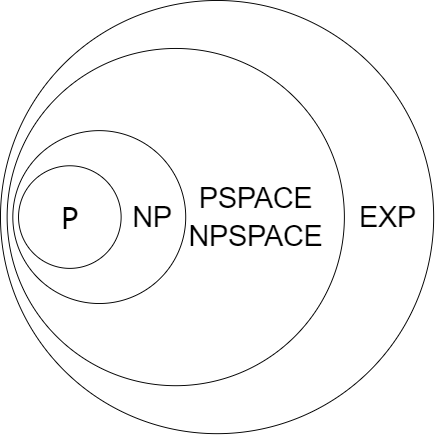
\includegraphics[scale = .3]{imm/Untitled Diagram.png}
\end{figure}


Abbiamo anche le classi $CO\_P$ e $CO\_NP$, ovvero le classi dei problemi complementari $P$ e $NP$. Si ha che, grazie al determinismo, cambiando semplicemente la risposta data in output, possiamo dire $CO\_P=P$\\
Quando si introduce il non determinismo le cose cambiano. La domanda iniziale era del tipo \textit{esiste almeno uno} quindi il completamento è \textit{non esiste nessuno}, quindi devo verificare tutti i casi, andando in un caso che nemmeno la NDTM riesce a risolvere, si finisce infatti nella classe $EXP$. \\ Quindi si ha che:
$P\subseteq CP\_NP\land P\subseteq NP$ non avendo un rapporto diretto e definito tra $NP$ e $CO\_NP$.

\part{Esercitazioni - Rizzi}
\section{Introduzione al Pattern Matching su stringhe}
%non centra un cazzo con le lezioni frontali
Il \textbf{pattern matching} si occupa di ricercare un all'interno di un testo $T$ le occorrenze di un pattern $P$. Si hanno: 
\begin{itemize} 
    \item pattern matching esatto: trovare le occorrenze esatte di $P$ in $T$
    \item pattern matching approssimato : trovare le occorrenze approssimate di $P$ in $T$
\end{itemize}
\subsection{Definizioni}
Definiamo stringa come una sequenza di simboli appartenenti ad un dato alfabeto $\Sigma$, scritta come: \\
$X= x_1,\ldots,x_n,\quad \forall x_i\in \Sigma, \forall i = 1, \dots, n$ ovviamente non è necessario che la stringa contenga tutti i simboli dell'alfabeto.\\ 
Diamo alcune definizioni utili: 
\begin{itemize} 
    \item $|X|$ indica la lunghezza della stringa 
    \item $\varepsilon$ indica la stringa vuota, di lunghezza 0
    \item $X[i]$ indica il carattere all'indice $i$ di $X$ (partendo da 1 e non da 0) 
    \item $X[i,j]$ indica la sottostringa che parte dall'indice $i$ e arriva all'indice $j$ (estremi inclusi).  \\
    Inoltre se si hanno $i\neq j$ e $j\neq |X|$ si ha una \textbf{sottostringa propria}.\\ 
    (Esempio: per $X=bbaccbbaac$ ho la sottostringa $X[4,8]=ccbba$) 
    \item $X[1,j]$ indico un \textbf{prefisso} di $X$ di lunghezza $j$ (estremo incluso). 
    Si parla di \textbf{prefisso proprio} se $j \neq |X|$, se $j=0$ allora si ha \textbf{prefisso nullo} e si indica con $\varepsilon$.\\
    \item $X[i,|X|]$ indica un \textbf{suffisso} della stringa $X$ di lunghezza $|X|-i+1$. 
    Si ha inoltre che se ho $X[|X|,|X|+1]$ allora ho il \textbf{suffisso nullo}, ovvero $\varepsilon$.\\ 
\end{itemize}
\subsection{Pattern Matching Esatto (PME)}
Preso in input un testo $T$ di lunghezza $n$ e un patter $P$ di lunghezza $m$, definiti all'interno dell'alfabeto $\Sigma$, l'algoritmo di restituisce tutte le occorrenze esatte di $P$ in $T$.\\ 
$P$ occorre esattamente in posizione i di $T$,se la sottostringa $T[i, i+|P|-1]$  coincide con  $P$. Quindi in output ho tutte le posizione $i$ nel testo tali per cui $T[i,i+m-1]$ è esattamente uguale a $P$.

\subsubsection{Algoritmo banale per PME esatto}
Una finestra $W$ lunga $m = |P|$ scorre lungo $T$ da sinistra a destra a partire dalla posizione $i = 1$. Nella generica posizione $i$ di $W$ ognuno dei simboli di $P$ viene confrontato con il corrispondente simbolo di $T$ all'interno di $W$ procedendo da sinistra verso destra. Se ogni simbolo di $P$ è uguale al suo corrispondente in $W$, allora viene prodotta in output l'occorrenza $i$ di $P$ in $T$. In caso contrario la finestra $W$ viene spostata alla posizione $i+1$ e il confronto riparte. Tale algoritmo ha una complessità $\mathcal{O}(|T| \cdot |P|)$.


\subsection{Pattern Matching Approssimato (PMA1)}
Preso in input un testo $T$ di lunghezza $n$ e un pattern $P$ di lunghezza $m$, definiti su alfabeto $\Sigma$, e una soglia di errore $k$, riporta come output tutte le occorrenza approssimate di $P$ in $T$. 
Bisogna fare riferimento alla \textbf{Distanza di edit}
\subsubsection{Distanza di edit}
Date due stringhe $X_1$ e $X_2$ si definisce distanza di edit il minimo numero di operazioni di sostituzione, cancellazione e inserimento di un simbolo che trasformano $X_1$ in $X_2$ (o viceversa). La distanza di edit tra due stringhe è simmetrica.
\subsubsection{Occorrenza approssimata}
Date due stringhe $T$ e $P$, definite sull'alfabeto $\Sigma$, e una soglia $k$, si dirà che:
\begin{itemize}
    \item $P$ ha un’occorrenza approssimata in $T$ in posizione $i$ se esiste (almeno) una sottostringa $T[i-L+1,i]$ che finisce in posizione $i$, e ha distanza di edit al più $k$ con $P$. 
    \item $L$ è un certo valore non prevedibile in quanto sto ammettendo che il match sia su una stringa di lunghezza diversa da quella del pattern
    \item l'output diventa l'insieme di tutte le posizioni $i$ di $T$in cui finisce almeno una sottostringa che ha con $P$ una distanza di edit al più $k$.
\end{itemize}
Definiamo \textbf{bordo} della stringa $X$, $B(X)$, che è il più lungo prefisso proprio che occorre come suffisso di $X$.
Il bordo è per definizione un prefisso proprio e non può coincidere con l’intera $X$ \\ 
Definiamo concatenazione tra una stringa $X$ e un simbolo $\sigma$ come: $X\sigma$

\subsection{Ricerca esatta con Automa a Stati Finiti}
Siamo nell'ambito del pattern matching esatto.\\
L'algoritmo utilizzato funziona nel seguente modo :
\begin{itemize}
    \item Abbiamo una fase di preprocessamento in tempo $\mathcal{O}(m|\Sigma|)$, per calcolare la funzione di transizione $\delta$.
    \item Usa la funzione di transizione per scandire  il testo in un tempo lineare nella sua lunghezza $\mathcal{O}(n)$ per cercare tutte le occorrenze esatte del pattern $P$. 
\end{itemize}

\subsubsection{Funzione di transizione}
Definiamo $\delta$ definita sul pattern $P$ come: $\delta:\{0,1,\ldots, m\}\times \Sigma\to\{0,1,\,\ldots, m\}$  \\
Quindi ad ogni coppia di valori che possiamo formare tra un simbolo e un intero tra 0 e $m$, corrisponde un intero tra 0 e $m$. Nel dettaglio si hanno due casi:
\begin{enumerate}
    \item $\delta(j,\sigma) = j + 1 \iff j < m \land P[j + 1]= \sigma$, dove $\sigma$ è l'input della funzione.
    \item $\delta(j,\sigma) = k \iff P[j + 1]\neq \sigma \lor j = m,\mbox{ con } k = |B(P[1, j] \sigma)|$. 
    on $k$ che è la lunghezza del bordo tra il prefisso corrente a cui viene concatenato il carattere $\sigma$. Si ha che $k\leq j$ per definizione (dato che sto calcolando il bordo su una stringa di lunghezza $j+1$).  
\end{enumerate}
La transizione dallo stato $j$ allo stato $\delta(j,\sigma)$ avviene attraverso il simbolo $\sigma$. 

%%%%HA FATTO MOLTI ESEMPI, CI STANNO

Facciamo due osservazioni:
\begin{enumerate}
    \item dallo stato 0, si arriva allo stato 0 per qualsiasi simbolo $\sigma\neq P[1]$ e quindi si arriva allo stato 1 attraverso $\sigma =P[1]$ 
    \item dallo stato $m$ si arriva sempre ad uno stato $k\leq m$ e da uno stato $m$ si può arrivare di nuovo ad uno stato $m$
\end{enumerate}


%%%%HA FATTO MOLTI altri ESEMPI, CI STANNO

\section{Lezione del 17}
\subsection{Scansione del testo}
La ricerca di $P$ in $T$, partendo da uno stato iniziale $s_0 = 0$, avviene leggendo il testo $T$ dal simbolo in posizione 1 al simbolo in posizione $n$. \\  
Ad ogni posizione $q$ da 1 a $n$ è associato uno stato $s_q$, ottenuto effettuando la transizione dallo stato $s_{q-1}$ tramite il simbolo $T[q]$.\\

Si supponga che l’algoritmo abbia appena letto il simbolo $T[q]$ e che stia per effettuare la transizione dallo stato $s_{q-1}$ a $s_q$.\\
Si supponga che $j$ sia la lunghezza del più lungo prefisso di $P$ che ha un’occorrenza in $T$ che finisce in posizione $q-1$ (e che inizia quindi in posizione $q-j$).\\
Si supponga che $j$ sia lo stato $s_{q-1}$ a cui l’algoritmo arriva dopo aver letto il simbolo $T[q-1]$. \\
L’algoritmo dopo aver letto il simbolo $T[q]$, passa al nuovo stato $s_q = \delta(j, T[q])$.\\
Il calcolo di $s_q = \delta(j, T[q])$ dipende dal verificarsi di uno dei seguenti casi:
\begin{enumerate}
    \item caso 1: $j<m$ e $P[j+1] = T[q]$	(in posizione $j+1$ del pattern, c’è lo stesso simbolo appena letto nel testo)\\
    Questo significa che quando mi trovo in $P$ in posizione $j+1$, trovo lo stesso carattere presente in $T$ in posizione $q$: $s_q = j+1$		\\
    In poche parole stiamo dicendo che $P[1, j+1]$ ha un’occorrenza in $T$ che inizia in $q-j$ e finisce in $q$, significa che il matching si amplifica ma la posizione di partenza resta medesima. \\
    
    La transizione da uno stato $j$ allo stato successivo $j+1$, dopo aver letto il simbolo $T[q]$, implica che il prefisso $P[1,j+1]$ ha un’occorrenza su $T$ che inizia in posizione $q-(j+1)+1$. Che in termini di conti non cambia nulla, ma viene specificato il punto di arriva che non è più $j$, bensì $j+1$, e sapendo che si parte comunque dalla posizione $q-j$ bisogna fare i giusti aggiustamenti. E questo rappresenta il caso generale.\\
    
    
    In particolare per $j+1= m$:
    La transizione da uno stato $m-1$ allo stato successivo $m$, dopo aver letto il simbolo $T[q]$, implica che il prefisso $P[1,m] = P$ ha un’occorrenza su $T$ che inizia in posizione $q-(m)+1$.
    \item caso 2: $j=m$ oppure $P[j+1] \neq T[q]$. Semplifichiamo questo caso introducendo due casi in cui andiamo a valutare separatamente le due possibili componenti.
    
    \begin{enumerate}
        \item $j < m$ e $P[j+1] \neq T[q]$	(in posizione $j+1$ del pattern, c’è un simbolo diverso da quello appena letto nel testo)\\
        La configurazione in questo caso ci dice $s_q = k$, dove $k$ è la lunghezza del bordo di $P[1,j]T[q]$\\		
        $P[1,k]$ ha un’occorrenza in $T$ che inizia in $q-j$ (che viene scartata perché già controllata) e un’altra che inizia in $q-k+1$ e che finisce in $q$.\\
        La transizione da uno stato $j$ allo stato $k \leq j$, dopo aver letto il simbolo $T[q]$, implica che il prefisso $P[1,k]$ ha un’occorrenza su $T$ che inizia in posizione $q-k+1$.
        
        \item $j = m$	(il più lungo prefisso del pattern che ha un’occorrenza nel testo che finisce in $q-1$ è tutto il pattern; il pattern occorre in posizione $q-j = q-m$)\\
        Esiste un’occorrenza di $P$ in $T$ che finisce in $q-1$. In questo caso abbiamo $s_q = k$, dove $k$ è la lunghezza del bordo di $P[1,m]T[q]$\\
        $P[1,k]$ ha un’occorrenza in $T$ che inizia in $q-m$ e un’altra che inizia in $q-k+1$ e finisce in $q$. \\
        La transizione da uno stato $j=m$ allo stato $k \leq m$, dopo aver letto il simbolo $T[q]$, implica che il prefisso $P[1,k]$ ha un’occorrenza su $T$ che inizia in posizione $q-k+1$.\\
        
        È possibile passare da uno stato $m$ a uno stato $m$ tramite $T[q]$.\\
        Lo stato iniziale $m$ indica un’occorrenza di $P$ in $T$. Lo stato di arrivo $k$ è sicuramente $\leq m$. Se $k=m$, allora esiste una nuova occorrenza di $P$ in $T$ che risulta essere sovrapposta con la precedente di $m-1$ simboli.
        \end{enumerate} 
\end{enumerate}

I tre casi (1, 2(a) e 2(b)) possono essere generalizzati: partendo dallo stato $s_{q-1} = j$, con $j \leq m$, dopo aver letto il simbolo $T[q]$, si passa a $s_{q} = f$, con $f \leq m$.
Il prefisso $P$ di lunghezza $f$ occorre in $T$ in posizione $q-f+1$.\\
Se $f=m$, allora $P$ occorre in $T$ alla posizione $q-m+1$.

\subsection{Scansione del testo}
I passi da eseguire per portare a termine il quesito sono:
\begin{enumerate}
    \item Si parte dallo stato iniziale $s_0=0$ e si effettua una scansione di $T$ dal primo all’ultimo simbolo. 
    \item Per ogni posizione $q$ di $T$ si effettua una transizione dallo stato corrente $s$ al nuovo stato $f=\delta(s, T[q])$.
    \item Ogni volta che il nuovo stato $f$ coincide con $m$, viene prodotta in output l’occorrenza $q-m+1$.
\end{enumerate}

\begin{lstlisting}
    Procedure scan-text(delta, T, m)
    begin
        n <- |T|
        s <- 0						//stato corrente
        for q <- 1 to n do 
            f <- delta(s,T[q])
            if f = m then
                output q-m+1		//occorrenza di P in T
		s <- f
    end
\end{lstlisting}


Complessità: $\mathcal{O}(n)$.

\subsection{KMP (Knuth-Morris-Pratt)}

\textbf{Algoritmo}:\\
\begin{enumerate}
    \item Preprocessing in tempo $\mathcal{O}(m)$ del pattern $P$ di lunghezza $m$, tramite il calcolo della prefix-function $\varphi$ (funzione di fallimento).
    \item Scansione in tempo $\mathcal{O}(n)$ del testo $T$ di lunghezza $n$ per ricercare le occorrenze esatte di $P$.
\end{enumerate}

Dato il pattern $P$ di lunghezza $m$, la prefix-function $\varphi : \{0, \dots, m\} \to \{-1, \dots, m-1\}$ è tale che:
\begin{enumerate}
    \item se $1 \leq j \leq m$, allora $\varphi (j) = |B(P[1,j])|$
    \item se $j=0$, allora $\varphi (j) = -1$.
\end{enumerate}
\section{Ricerca esatta con KMP}
\subsection{Bordo di una stringa}
\subsubsection{Definizione non ricorsiva di bordo di una stringa}
Il bordo di una stringa $X$ è il più lungo prefisso proprio di $X$ che è anche uguale a un suffisso di $X$.

\subsubsection{Definizione ricorsiva di bordo di una stringa}
Il bordo della stringa vuota è la stringa vuota stessa: $B(\varepsilon) = \varepsilon$.\\
Il bordo di una stringa composta da un solo simbolo è la stringa vuota: $B(\sigma) = \varepsilon$.\\
Il bordo $B(X\sigma)$ della concatenazione tra una stringa $X$ e un simbolo $\sigma$ è: 
\begin{itemize}
    \item $B(X\sigma) = B(X)\sigma$, se $\sigma$ è il simbolo di $X$ in posizione $|B(X)|+1$
    \item $B(X\sigma) = B(B(X)\sigma)$, se $\sigma$ non è il simbolo di $X$ in posizione $|B(X)|+1$
\end{itemize}

\subsection{Calcolo di \texorpdfstring{$\varphi$}{} per induzione}
Per $j=0$ e $j=1$ il calcolo è immediato: $\varphi(0) = -1$ e $\varphi(1) = 0$. \\
Per calcolare $\varphi(j)$ per $j>1$, si suppone che $\varphi$ sia nota per tutti gli indici precedenti tra $0$ e $j-1$. \\

Se prendiamo in considerazione ad esempio una stringa $P$, di lunghezza $j$ dobbiamo sapere come ci comportiamo alla posizione $j-1$ per sapere come calcolare la nostra  $\varphi$.
Quindi il probleam si pone nei termini seguenti $P[1,j] = P[1, j-1]P[j]$. Quindi, teoricamente, siamo in grado di calcolare $\displaystyle \varphi$ facendo \[\varphi(j)=|B(P[1,j])| = |B( P[1, j-1]P[j])|\]
Dove:
\begin{itemize}
    \item $P[1, j-1]$ sarà la nostra $X$ vista in precedenza
    \item $P[j]$ è invece la nostra $\sigma$
\end{itemize}
Questo ci porta ad avere il bordo come espresso in precedenza $B(X\sigma)$

Per definizione:  
\begin{itemize}
    \item $|B(P[1,j-1])| = k_1 = \varphi(j-1) \implies B(P[1, j-1]) = P[1, k_1]$
    \item $|B(P[1,k_1])| = k_2 = \varphi(k_1) = \varphi(\varphi(j-1)) \implies B(P[1,k_1]) = P[1, k_2]$
    \item $|B(P[1, k_2])| = k_3 = \varphi(k_2) = \varphi(\varphi(k_1)) = \varphi(\varphi(\varphi(j-1)))$
\end{itemize}
Per applicare la definizione ricorsiva per il calcolo di $\varphi(j)$ io devo prevedere due casi:
\begin{itemize}
    \item \textbf{Caso 1}: $P[k_1 + 1] = P[j]$, significa che $\sigma$ appare immediatamente dopo il bordo di $X$, quindi il simbolo $\sigma$, che nel nostro caso è $P[j]$, è uguale a $P[k_1 + 1]$. Questo lo possiamo suddividere in alcuni sottocasi:
        \begin{itemize}
            \item $B(P[1, j-1] P[j]) = B(P[1, j-1]) P[j] \implies |B(P[1, j-1] P[j])| = |B(P[1, j-1])| +1$. Quello che ci dice la nostra definizione, è che questo è di conseguenza uguale a $k_1 + 1 = \varphi(j-1) + 1$.
        \end{itemize}
    \item \textbf{Caso 2}: $P[k_1 + 1] \neq P[j]$, significa che $\sigma$ non appare immediatamente dopo il bordo di $X$, quindi il simbolo $\sigma$, che nel nostro caso è $P[j]$, non è uguale a $P[k_1 + 1]$.
        \begin{itemize}
            \item $B(P[1, j-1] P[j]) = B(B(P[1, j-1]) P[j])$. Sappiamo che nella definizione del bordo abbiamo detto che $B(P[1, j-1]) = k_1 = \varphi(j-1)$. Possiamo eseguire allora delle sostituzioni, raggiungiamo quindi: $B(B(P[1, j-1]) P[j]) = B(P[1,k_1]P[j])$
            \item Andando avanti con le considerazioni, la stessa che ci ha portati a dire  $B(P[1, j-1]) = k_1$, ottenendo in modo ricorsivo che  $B(P[1, k_1]) = k_2 = \varphi(k_1) = \varphi(\varphi(j-1))$, sempre per definizione del bordo. 
        \end{itemize}
        Con quanto eseguito fin'ora, ci rendiamo conto che il caso 2, vada ulteriormente diviso, trovando.
        \begin{enumerate}
            \item $P[k_1 + 1] \neq P[j] \land P[k_2 + 1] = P[j]$ , eseguendo i passi visti in precedenza ci ritroviamo ad avere a che fare con $B(P[1, k_1])P[j]$. Per intenderci siamo nel caso di $B(X)\sigma$. Questo implica dire che $|B(P[1, j-1] P[j])| = |B(P[1, k_1])| + 1 $.\\
            Questo altro che non è, per come visto in precedenza, $|B(P[1, k_1])| + 1 = k_2 + 1$ che altro non è , per definizione, che $\varphi(k_1) +1 = \varphi(\varphi(j - 1)) +1$
            \item $P[k_1 + 1] \neq P[j] \land P[k_2 + 1] \neq P[j]$. Come nel caso visto prima $B(P[1, j-1] P[j]) = B(B(P[1, k_1]) P[j])$. Anche qui, per definizione, ci ritroviamoa  scrivere $B(P[1, k_2] P[j])$
        \end{enumerate}
\end{itemize}
Questi passaggi possono essere eseguiti fino a quando non ci ritroviamo a considerare il \[P[k_1 + 1] \neq P[j] \land P[k_2 + 1] \neq P[j] \land \dots \land P[k_{p}+1] (\neq)(=) P[j]\]

In generale, se si raggiunge un valore $k_p$ (con $p$ = numero di chiamate ricorsive) tale per cui $P[k_p + 1] = P[j]$, allora $\varphi(j) = k_p +1$.\\
Altrimenti, si raggiungerà a un certo punto un valore $k_p = -1$ che implica che il bordo di $P[1, j]$ è nullo e quindi $\varphi(j) = 0$ (cioè ancora uguale a $k_p +1$).

\subsubsection{Algoritmo di calcolo di \texorpdfstring{$\varphi$}{}}

\begin{lstlisting}
    phi(0) <- -1
    phi(1) <- 0
    j <- 2
    k <- phi(j-1)
    caso 1: P[k+1] = P[j]
	    phi(j) <- k+1
        j <- j + 1
        ritorno alla riga 4
    caso 2: P[k+1] != P[j]
        k <- phi(k)
        if k = -1
            phi(j) <- k+1
            j <- j+1
            ritorno alla riga 4
        else
        	ritorno a testare i due casi
\end{lstlisting}

\begin{lstlisting}
    Procedure Compute-Prefix-Function(P)
    begin
        m <- |P|
        phi(0) <- -1
        phi(1) <- 0
        for j <- 2 to m do
            k <- phi(j-1)
            while k >= 0 & P[k+1] != P[j] then
                k <- phi(k)
                phi(j) <- k+1
        return phi
    end
\end{lstlisting}


\subsection{Scansione del testo}
La scansione del testo $T$ alla ricerca di $P$ avviene tramite una finestra $W$ di confronto lunga $m$ che scorre lungo $T$ da sinistra a destra, e inizialmente è posizionata in corrispondenza della posizione $i=1$ di $T$.\\
Per ogni posizione $j$ di $W$, ogni simbolo di $P$ viene confrontato con il corrispondente simbolo del testo T in W, procedendo da sinistra a destra. \\
Se tutti i simboli sono confrontati con successo, allora nella posizione $i$ di $T$ esiste un’occorrenza esatta di $P$. La finestra viene poi spostata verso destra in una nuova posizione e si ripete il confronto.\\

La finestra $W$ viene spostata anche di più posizioni utilizzando la funzione $\varphi$.
Il confronto riparte dal simbolo del testo che aveva dato \textit{mismatch} con il pattern quando $W$ era nella presente posizione.

\subsubsection{Spostamento di W}
Si assuma che la finestra $W$ si trovi in posizione $i$ su $T$ e il primo carattere di $P$, che determina un \textit{mismatch} con $T$, sia in posizione $j>1$ (il simbolo di \textit{mismatch} su $T$ sarà quindi in posizione $i+j-1$).\\
Per definizione, il valore $k = \varphi(j-1)$ è la lunghezza del bordo del prefisso $P[1, j-1]$. Quindi $P[1,k]$ ha un’occorrenza su $T$ che inizia in posizione $i$ e una che inizia in $p=i+j-k-1 = i + j - \varphi(j-1) - 1$.\\

Il salto di $W$ da $i$ a $p$ garantisce di non perdere occorrenze di $P$ e che i primi $k = \varphi(j-1)$ simboli di $P$ abbiano un matching con $T$ a partire dalla nuova posizione $p$.

Il confronto tra i simboli di $T$ e di $P$ con $W$ nella nuova posizione $p$ può ripartire dalle posizioni: $i+j-1$ su $T$ e $k+1$ su $P$.

Quindi, $W$ viene spostata alla posizione $p = i+j-\varphi(j-1) -1$ e i primi $\varphi(j-1)$ simboli di $P$ non vengono più confrontati con i corrispondenti simboli su $T$.\\

Si devono considerare però alcuni casi particolari:
\begin{enumerate}
    \item $\varphi(j-1)=0$, il bordo è nullo \\
        $W$ viene spostata alla posizione $p = i+j-1$ e i primi $0$ simboli di $P$ non vengono più confrontati con i corrispondenti simboli su $T$.
        Quindi il confronto riparte dal simbolo in posizione $i+j-1$ su $T$ e dal primo simbolo su $P$.
    \item $j=1$, il \textit{mismatch} avviene sui primi due simboli di testo e pattern
        $W$ viene spostata alla posizione $p = i+j-\varphi(0) -1 = i + 1$ e i primi $\varphi(0) = 0$ simboli di $P$ non vengono più confrontati con i corrispondenti simboli su $T$. Quindi il confronto riparte dal simbolo in posizione $i+1$ su $T$ e dal primo simbolo su $P$.
    \item $j = m+1$, in posizione $i$ c’è un’occorrenza esatta del pattern
        $W$ viene spostata alla posizione $p = i+m-\varphi(m)$ e i primi $\varphi(m)$ simboli di $P$ non vengono più confrontati con i corrispondenti simboli su $T$. Quindi il confronto riparte dal simbolo in posizione $i+m$ su $T$ e dal simbolo in posizione $\varphi(m) + 1$ su $P$.
\end{enumerate}


\subsubsection{Pseudocodice della scansione del testo T}

\begin{lstlisting}
KMP(P,T,phi)
    begin
        m <- |P|
        n <- |T|
        j <- 0
        for q <- 1 to n do
            while j >= 0 & P[j+1] != T[q] then
                j <- phi(j)
            j <- j+1
            if j = m then
                return q-m+1
    end
\end{lstlisting}

Complessità: $\mathcal{O}(n)$.
\section{Ricerca esatta con algoritmo di Baeza-Yates e Gonnet (BYG) o paradigma SHIFT-AND}
Per tale algoritmo si hanno due fasi fondamentali:
\begin{enumerate}
    \item Preprocessig del pattern $P$ di lunghezza $m$ in tempo $\mathcal{O}(|\Sigma|+m)$, tramite il calcolo di una tabella $B$ di $|\Sigma|$ parole di $m$ bit. 
    \item Scansione del testo $T$ di lunghezza $n$ in tempo $\mathcal{O}(n)$ per cercare le occorrenze esatte di $P$.
\end{enumerate}
In questo caso abbiamo che $\Sigma$ altro non è che l'alfabeto di definizione del testo e del pattern. \\
L'algoritmo \textit{BYG} non funziona sul confronto di simboli ma si basa sul  paradigma SHIFT-AND compiendo operazioni su parole di bit.

\subsection{Operazioni usate da BYG}
\begin{itemize}
    \item  congiunzione: \textbf{AND} \\
    $w_1$ AND $w_2$ restituisce una parola $w$ tale che: $w[i]=1 \iff w_1[i]=1 \land w_2[i]=1$; $w[i] = 0$, altrimenti.
    \item  disgiunzione: \textbf{OR}\\
    $w_1$ OR $w_2$ restituisce una parola $w$ tale che: $w[i]=1 \iff w_1[i]=1 \lor w_2[i]=1$; $w[i] = 0$, altrimenti.
    \item  shift dei bit di una posizione a destra con bit più significativo uguale a 0: \textbf{RSHIFT}\\
    RSHIFT($w_1$) restituisce una parola $w$ tale che: $w[1]=0$ e $w[i] = w_1[i-1]$ se $2 \leq i \leq |w|$.
    \item  shift dei bit di una posizione a destra con bit più significativo uguale a 1: \textbf{RSHIFT1}\\
    RSHIFT1($w_1$) restituisce una parola $w$ tale che: $w[1]=1$ e $w[i] = w_1[i-1]$ se $2 \leq i \leq |w|$.

  È una combinazione di RSHIFT e OR: RSHIFT1($w_1$) = RSHIFT($w_1$) OR $100..0$.
\end{itemize}

\subsection{Tabella B}
Una \textit{parola} $B_{\sigma} = b_1 \dots b_m$, per $\sigma \in \Sigma$, è tale che $B_{\sigma}[i] = b_i = 1 \iff P[i] = \sigma$. \\ L’uguale a $1$ possono sparire perché i bit hanno in sé il concetto di verità e falsità. Quindi si potrebbe scrivere soltanto $B_{\sigma}[i] = b_i \iff P[i] = \sigma$.

La \textit{tabella} $B$ è l'insieme delle parole $B_\sigma$, $\forall \sigma \in \Sigma$. La costruzione della tabella permette di rispondere alla domanda: $P[i] = \sigma$?
\[P[i] = \sigma \iff B_{\sigma}[i] =1\]

L’uguale a 1 è omissibile perché trattando valori binari, essi contengono già il valore di verità.

\subsubsection{Algoritmo di calcolo della tabella B}
\begin{enumerate}
    \item Tutte le parole $B_\sigma$ vengono inizializzare a $m$ zeri.
    \item Viene inizializzata una parola $M$ (maschera) di $m$ bit tutti uguali a $0$ tranne il più significativo che è uguale a $1$. 
    \item Si esegue una scansione di $P$ da sinistra verso destra e per ogni posizione $i$: 
    \begin{enumerate}
        \item $B_{P[i]} = M$ OR $B_{P[i]}$
        \item $M = $ RSHIFT($M$)
    \end{enumerate}
\end{enumerate}

\begin{algorithm}[H]
\SetAlgoLined
\KwResult{the table B of the words $B\sigma$}
    $ m \leftarrow |P|$\;
    \For{each $\sigma \in \Sigma$}{
        $B\sigma \leftarrow 000\dots0$\;
    }
    $m \leftarrow 100\dots0$\;
    \For{$i \leftarrow 1$ to $m$}{
        $\sigma \leftarrow P[i]$\;
        $B\sigma \leftarrow M$ OR $B\sigma$\;
        $M = RSHIFT(M)$\;
    }
 \caption{Procedura Compute-B(P)}
\end{algorithm}


Complessità: $\mathcal{O}(|\Sigma|+m)$

\subsection{Scansione del testo}
Si seguono alcuni step:
\begin{enumerate}
    \item Il testo $T$ viene scandito dalla prima all’ultima posizione.
    \item Per ogni posizione $j$ del testo $T$ viene calcolata una parola $D_j$ di $m$ bit.
    \item Ogni volta che $D_j$ ha il bit meno significativo uguale a $1$, viene prodotta in output l’occorrenza esatta alla posizione $j-m+1$.
\end{enumerate}
Si denoti con $P[1, i] = suff(T[1, j])$ il fatto che $P[1,i]$ occorre esattamente come suffisso di $T[1,j]$.

\subsubsection{Definizione di parola \texorpdfstring{$D_j$}{}} 
Definiamo la parola $D_j$ ($0 \leq j \leq n$) nel seguente modo:
\[D_j = d_1 \dots d_m \mbox{ tale che } d_i = D_j[i] = 1 \iff P[1, i] = suff(T[1, j])\]
In particolare, per definizione, $D_0 = 00\dots 0$ ($\forall i, P[1,i] \neq suff(T[1,0])$).
Inoltre, $d_m = D_j[m] = 1 \iff P[1,m] = suff(T[1,j])$, ovvero se $P$ ha un’occorrenza in $T$ che inizia in $j-m+1$ e finisce in $j$.

\subsection{Scansione del testo}
Lo step di scansione del testo $T$ inizia dalla parola $D_0 = 00\dots0$. Per ogni $j$ da $1$ a $n$, calcola la parola $D_j$ a partire dalla parola $D_{j-1}$ (calcolata per $j-1$). Ogni volta che $D_j$ ha il bit più a destra uguale a $1$, viene prodotta in output la posizione $j-m+1$ dell’inizio di un’occorrenza di $P$ su $T$.

\subsubsection{Calcolo di \texorpdfstring{$D_j$}{} a partire da \texorpdfstring{$D_{j-1}$}{}}
\begin{itemize}
    \item Nel primo caso abbiamo che $i>1$\\
    \begin{equation*}
        \begin{split}
            D_j[i] = 1 &\iff  P[1,i] = \mbox{suff}(T[1,j]) \\
            & \iff P[1, i-1] = \mbox{suff}(T[1, j-1]) \land  P[i] = T[j]\\
            & \iff D_{j-1}[i-1] = 1 \land P[i] = T[j]\\
            & \iff D_{j-1}[i-1] = 1 \land B_{T[j]}[i] = 1
        \end{split}
    \end{equation*}
        Gli uguale a $1$ possono sparire perché i bit hanno in sé il concetto di verità e falsità, possiamo quindi riscivere che:
        \[D_j[i] = D_{j-1}[i-1]  \land B_{T[j]}[i]\]
    \item Dobbiamo valutare anche la possibilità in cui $i=1$ \\
    \begin{equation*}
        \begin{split}
        D_j[i] = 1  & \iff P[1,i] = \mbox{suff}(T[1,j]) \\
                    & \iff P[1] = T[j] \\ 
                    & \iff B_{T[j]}[1]=1
        \end{split}
    \end{equation*}
        Il risultato non cambia se si effettua l’AND logico con un bit uguale a $1$: \[D_j[i] \iff 1 \land B_{T[j]}[1]\]\\
        Tutto questo ci porta a poter dire che \[D_j[i] = 1 \land B_{T[j]} [1] \]
\end{itemize}
Alcune notazioni da ricordarsi, come definizioni raggiunte per il calcolo ricorsivo, per quando andiamo a calcolare la nostra $D_j$ sono:
\begin{itemize}
    \item $D_j[i] = D_{j-1}[i-1] \land B_{T[j]}[i]$
    \item $D_j[i] = 1 \land B_{T[j]} [1]$ 
\end{itemize}
I due punti eseguiti in tal modo, corrisponde a eseguire rispettivamente:
\begin{itemize}
    \item $D_j[i] =$ RSHIFT1($D_{j-1}$)$[i] \land B_{T[j]}[i]$
    \item $D_j[i] =$ RSHIFT1($D_{j-1}$)$[1] \land B_{T[j]} [1]$ 
\end{itemize}
Le due formule possono essere unite: $D_j[i] =$ RSHIFT1($D_{j-1}$)$[i] \land B_{T[j]}[i]$, per $i \geq 1$

\subsubsection{Scansione del testo}
L’algoritmo di scansione del di $T$ inizializza una maschera $M = 00 \dots 01$ di $m$ bit tutti uguali a $0$ tranne quello più a destra che è uguale a $1$ e inizializza la parola $D_0 = 00\dots 0$.\\
Per $j$ compreso tra $1$ e $n$, calcola la parola $D_j = $ RSHIFT1($D_{j-1}) \land B_{T[j]}$.
Ogni volta che la parola ($D_j \land M$) è uguale a $00 \dots 01$, viene prodotta in output la posizione $j-m+1$ dell’inizio di un’occorrenza di $P$ su $T$. 


\begin{algorithm}[H]
\SetAlgoLined
    $ B \leftarrow $ Compute-B(P)\;
    $n \leftarrow |T|$\;
    $D \leftarrow 00\dots00$\;
    $M \leftarrow 00\dots01$\;
    \For{$j \leftarrow 1 $ to $n$}{
        $\sigma \leftarrow T[j]$\;
        $D \leftarrow RSHIFT1(D) \land B\sigma$\;
        \If{$(D \land M) == 00\dots01$}{
            return $j-m+1$
        }
    }
 \caption{Procedura BYG(P,T)}
\end{algorithm}



Complessità: $\mathcal{O}(|\Sigma| + m + n)$
\section{Ricerca approssimata con algoritmo di Wu e Manber }
Prima di procedere andiamo a riprendere il concetto di occorrenza approssimata:
Dato un pattern $P$ e un testo $T$, definiti sull'alfabeto $\Sigma$, e una soglia di errore k, diciamo che:
\begin{teorema}{Occorrenza approssimata}{}
    P ha un'occorrenza approssimata in T, in posizione j se esiste una $T[j-L+1, j]$ che ha disatanza di edit con P al più pari a k. (occorrenza con al più k errori)
\end{teorema}
Questa tipologia di ricerca, in particolar modo con questo algoritmo, è basata su paradigma SHIFT-AND visto nella lezione precedente. Anche qui abbiaimo una suddivisione dei compiti in due fasi:
\begin{itemize}
    \item Preprocessing del pattern $P$ di lunghezza $m$ in tempo $\mathcal{O}(|\Sigma|+m)$, tramite il calcolo di una tabella $B$ di $|\Sigma|$ parole di $m$ bit.
     Il preprocessing è identico a quella della ricerca esatta di BYG.
     \item  Scansioni del testo $T$ di lunghezza $n$ in tempo $\mathcal{O}(nk)$ per cercare le occorrenze approssimate di $P$.
\end{itemize}
Dove $\Sigma$ è l’alfabeto di definizione del testo e del pattern. L’algoritmo WM è basato sul paradigma SHIFT-AND e opera su word di bit.\\

\subsection{Scansione del testo}
L’algoritmo effettua $k+1$ iterazioni di scansione del testo $T$ per $0 \leq h \leq k$, dove l’iterazione $h$ trova tutte le occorrenze del pattern $P$ con al più $h$ errori.
\begin{itemize}
    \item Tutte le occorrenze con al più $0$ errori sono trovate all’iterazione $h=0$ (occorrenze esatte).
    \item Tutte le occorrenze con al più $1$ errori sono trovate all’iterazione $h=1$.
\end{itemize}
\[\vdots\]
\begin{itemize}
    \item Tutte le occorrenze con al più $k$ errori sono trovate all’iterazione $h=k$.
\end{itemize}

La generica iterazione $h$ calcola $n$ parole $D_j^h$ lunghe $m$ bit tali che $D_j^h[m] = 1 \iff P$ ha un’occorrenza che finisce in $j$ con al più $h $ errori.  \\
L’iterazione $h=0$ calcola $n$ parole $D_j^0$ lunghe $m$ bit tali che $D_j^0[m] = 1 \iff P$ ha un’occorrenza che finisce in $j$ con al più $0$ errori. \\
L’iterazione $h=k$ calcola $n$ parole $D_j^k$ lunghe $m$ bit tali che $D_j^k[m] = 1 \iff P$ ha un’occorrenza che finisce in $j$ con al più $k$ errori. \\
Solo l’ultima iterazione $h=k$ produce in output tutte le posizioni $j$ su $T$ in cui finisce un’occorrenza di $P$ con al più $k$ errori.\\

\subsubsection{Parola \texorpdfstring{$D^h_j$}{}}
Si denoti con $P[1, i] = \mbox{suff}_h(T[1, j])$ il fatto che $P[1, i]$ occorre come suffisso di $T[1, j]$ con al più $h$ errori.

Quando si parla di definizione di parola $D^h_j$, lo si deve considerando i valori di $j$ e $h$ nel seguente modo: $0 \leq j \leq n, 0\leq h \leq k$\\
$D^h_j = d_1 d_2 \dots d_m$ tale che $d_i = D^h_j[i] = 1 \iff P[1, i ] = \mbox{suff}_h(T[1, j])$\\

In particolare, per definizione la parola $D^h_0$ è tale che:
\begin{itemize}
    \item $D^h_0 [i] = 1$, $\forall i \leq h$ (per le prime $h$ posizioni da sinistra) 
    \item $D^h_0[i] = 0$, $\forall i > h$ (per le ultime $m-h$ posizioni da destra)
\end{itemize}

Infatti si ha che: $\forall i \leq h$, $P[1, i] = \mbox{suff}_h(T[1,0])$ e $\forall i > h$, $P[1, i] \neq \mbox{suff}_h(T[1,0])$.\\

La parola $D^0_0$ (per $ h=0$) è per definizione $D^0_0 = 00..00$.\\

Inoltre $d_m = D^h_j[m] = 1 \iff P[1, m] = \mbox{suff}_h(T[1,j])$, ovvero se $P$ ha un’occorrenza che finisce in $j$ con al più $h$ errori (e quindi con al più $k$ errori).
$D^h_j[m] = 1 \implies D^k_j[m] = 1$

La parola $D^0_j = d_1 \dots d_m$ è tale che $d_j = D^0_j[i] = 1 \iff P[1,i] = \mbox{suff}(T[1,j])$.\\
La parola $D^0_j$ coincide con la parola $D_j$ dell’algoritmo di ricerca esatta di Baeza-Yates e Gonnet.

\subsubsection{Scansione del testo}
Alla prima iterazione $h = 0$, $T$ viene scandito per $j$ da $ 1$ a $n$ per calcolare tutte le parole $D^0_j$, come nell’algoritmo di BYG.\\

Alla generica iterazione $h > 0$, per ogni posizione $j$ del testo $T$ viene calcolata la parola $D^h_j$. All’ultima iterazione $h=k$ ogni volta che la parola calcolata $D^k_j$ ha il bit meno significativo uguale a $1$, viene prodotta in output la posizione $j$ in cui finisce un’occorrenza approssimata del pattern con al più $k$ errori.\\

Si vuole calcolare la generica parola $D^h_j$ per un qualsiasi $j>0$ e un qualsiasi $h>0$.
\begin{itemize}
   \item $h>0 \land j>0 \land i >1$
       In questa situazione abbiamo la possibilità di incontrare diverse casistiche:
       \begin{enumerate}
       \item In un primo caso ci ritroviamo a dire che:
           \begin{equation*}
               \begin{split}
                   D^h_j[i] = 1 &\iff P[1, i] = \mbox{suff}_h(T[1, j]) \\
                   & \Leftarrow P[1, i-1] = \mbox{suff}_h(T[1, j-1]) \land P[i] = T[j] \\
                    &\iff D^h_{j-1}[i-1] = 1 \land P[i] = T[i] \\
                    &\iff D^h_{j-1}[i-1] = 1 \land B_{T[j]}[i] = 1
               \end{split}
           \end{equation*}
           Con $\Leftarrow$ andiamo ad intendere che tutte le condizioni in $\iff$ devono essere verificate finché $D^h_j[i] = 1 \iff P[1, i] = \mbox{suff}_h(T[1, j])$ risulti corretto. Sarebbe una doppia implicazione. Ci ritroviamo quindi con:
           \[D^h_j[i] \Leftarrow D^h_{j-1}[i-1] \land B_{T[j]} [i]\]
       \item In un secondo caso invece:
            \begin{equation*}
               \begin{split}
               D^h_j[i] = 1 & \iff P[1, i] = \mbox{suff}_h(T[1, j]) \\
               & \Leftarrow P[1, i-1] = \mbox{suff}_{h-1}(T[1, j-1]) \\
               & \iff D^{h-1}_{j-1}[i-1] = 1
               \end{split}
            \end{equation*}
            In questo caso $P[i]$ e $T[j]$ possono anche essere diversi perché si rimane comunque nella soglia massima di $k$ errori. Quindi \[D^h_j[i] \Leftarrow D^{h-1}_{j-1}[i-1]\]
        \item Il terzo caso invece genera un errore:
        \begin{equation*}
            \begin{split}
                D^h_j[i] = 1 &\iff P[1, i] = \mbox{suff}_h(T[1, j]) \\
                & \Leftarrow P[1, i] = \mbox{suff}_{h-1}(T[1, j-1]) \\
                & \iff D^{h-1}_{j-1}[i] = 1
            \end{split}
        \end{equation*}
            Il suffisso è con $h-1$ perché $T[j]$ genera un errore.
            Quindi \[D^h_j[i] \Leftarrow D^{h-1}_{j-1}[i]\]
        \item Il quarto caso è solamente un duale del terzo caso :
        \begin{equation*}
            \begin{split}
                D^h_j[i] = 1 &\iff P[1, i] = \mbox{suff}_h(T[1, j])\\
                & \Leftarrow P[1, i-1] = \mbox{suff}_{h-1}(T[1, j]) \\
                & \iff D^{h-1}_{j}[i-1] = 1
            \end{split}
        \end{equation*}
             Quindi \[D^h_j[i] \Leftarrow D^{h-1}_{j}[i-1]\]
        \end{enumerate}
        Quindi per $i >1$, ci ritoviamo ad avere:
        \begin{equation*}
            \begin{split}
                D^h_j[i] & \iff  (D^h_{j-1}[i-1] \land B_{T[j]}[i]) \lor D^{h-1}_{j-1}[i-1] \lor D^{h-1}_{j-1}[i] \lor D^{h-1}_{j}[i-1] \\
                D^h_j[i] &=  (D^h_{j-1}[i-1] \land B_{T[j]}[i]) \lor D^{h-1}_{j-1}[i-1] \lor D^{h-1}_{j-1}[i] \lor D^{h-1}_{j}[i-1]
            \end{split}
        \end{equation*}
    \item $h>0 \land j>0 \land i = 1$\\
        Per $h>0 \land j>0$, $P[1,1]$ occorre sempre come suffisso del prefisso $T[1,j]$ (non nullo) con al più $h$ errori: $D^h_j[1]=1$, per $h>0 \land j>0$.\\
        
        Si sostituisce $i=1$ nella formula di calcolo di $D^h_j[i] \mbox{, con} i>1$: 
        \[D^h_j[1] = (D^h_{j-1}[0] \land B_{T[j]}[1]) \lor D^{h-1}_{j-1}[0] \lor D^{h-1}_{j-1}[1] \lor D^{h-1}_{j}[0]\]
        Si sostituisce al posto di tutti gli accessi ai bit in posizione $0$ un $1$: \[D^h_j[1] = (1 \land B_{T[j]}[1]) \lor 1 \lor D^{h-1}_{j-1}[1] \lor 1\]
\end{itemize}
Si effettua un RSHIFT1 sulle parole che nel caso $i=0$ andavano ad accedere ai bit in posizione $0$.\\
Così facendo è possibile unificare i due casi e ottenere: per $i \geq 1$, 
\begin{equation*}
    \begin{split}
        D^h_j[i] = & \left(\mbox{RSHIFT1}(D^h_{j-1})[i] \land B_{T[j]}[i]\right) \lor \\
        & \mbox{RSHIFT1}(D^{h-1}_{j-1})[i] \lor\\ 
        &  D^{h-1}_{j-1}[i]  \lor\\
        & \mbox{RSHIFT1}(D^{h-1}_{j})[i]
    \end{split}
\end{equation*}
Possiamo tranquilamente andare a rimuovere il calcolo sul bit a bit $[i]$ dato che sappiamo che sia il modo di agire, otteniamo:
\begin{equation*}
    \begin{split}
        D^h_j = & \left(\mbox{RSHIFT1}(D^h_{j-1}) \land B_{T[j]}\right) \lor \\
        & \mbox{RSHIFT1}(D^{h-1}_{j-1}) \lor\\ 
        &  D^{h-1}_{j-1}  \lor\\
        & \mbox{RSHIFT1}(D^{h-1}_{j})
    \end{split}
\end{equation*} 
\subsubsection{Scansione del testo}
\begin{enumerate}
    \item Inizializzazione di una maschera $M = 00\dots01$ di $m$ bit tutti a $0$ tranne il meno significativo che è uguale a $1$.
    \item Inizializzazione della parola $D^0_0 = 00\dots00$.
    \item Calcolo di $D^0_j$ per $j$ da $1$ a $n$ (algoritmo BYG).
    \item Per $h$ da $1$ a $k$: 
    \begin{itemize}
        \item Inizializzazione di $D^h_0$.
        \item Per $j$ da $1$ a $n$, calcolo di $D^h_j$
        \item Se $h=k$ e $(D^k_j \land M) \neq 0$, allora viene prodotta in output l’occorrenza $j$. 
    \end{itemize}
\end{enumerate}
\subsubsection{Proprietà}
\begin{itemize}
    \item $D^h_j[i]=1 \implies D^{h'}_j[i] = 1$, con $h' > h$
    \item $D^h_j[i] = 1 \implies D^{h+1}_j[i+1] = 1$, per $i<m$ e analogamente  $D^h_j[i] = 1 \implies D^{h+1}_j[i-1] = 1$, per $i>1$
    \item $|B(P)| = i \iff D_j[m] = 1$ e $i$ è la più grande posizione $< m$ tale che $D_j[i]=1$.
\end{itemize}
\section{Strutture di indicizzazione di un testo}
\begin{teorema}{Struttura di indicizzazione}{}
Struttura dati che riorganizza un testo in maniera da rendere facile ed efficiente un compito che compiuto sul testo originale risulta essere difficile e inefficiente.
\end{teorema}
Occorre innanzitutto: 
\begin{itemize}
    \item fissare un ordinamento dei simboli dell’alfabeto $\Sigma$ del testo (ordinamento lessicografico).
    \item estendere l’alfabeto $\Sigma$ con un simbolo sentinella, considerato lessicograficamente minore di tutti gli altri simboli ($\$$).
    \item aggiungere la sentinella alla fine del testo.
\end{itemize}

\subsection{Suffisso}
Il suffisso di indice $j$ è il suffisso $T[j, |T|]$ che inizia in posizione $j$ di $T$.
Se $j=|T|$, $T[j, |T|] = \$$, detto suffisso nullo.

Fissato l’ordine lessicografico dei simboli di $\Sigma$, si può stabilire l’ordinamento dei suffissi di $T$.

\subsubsection{Regola per ordinare due suffissi \texorpdfstring{$s_1$}{} e \texorpdfstring{$s_2$}{}}
Sia $i$ la prima posizione a sinistra tale che $s_1[i] \neq s_2[i]$.
\[s_1[i] < s_2[i] \implies s_1 < s_2\]
\[s_1[i] > s_2[i] \implies s_1 > s_2\]

La sentinella serve per non avere due suffissi uguali e per non avere che un suffisso sia suffisso di un altro.

\subsubsection{Rotazione}
La rotazione di indice $j$ è la concatenazione del suffisso $T[j, |T|]$ con il prefisso $T[1, j-1]$.

\subsection{Suffix Array (SA)}

Il suffix array di un testo $T$ di lunghezza $n$ è stato proposto da Myers e Manber (1990) e occupa $\mathcal{O} (n \log n)$ in spazio, permettendo la ricerca esatta di un pattern di lunghezza $m$ in un testo in tempo $\mathcal{O}(m \log n)$.
Inoltre, non contiene informazioni sui simboli del testo.

\begin{teorema}{Suffix Array}{}
Il Suffix Array di un testo $T$ ($\$$-terminato) di lunghezza $n$ è un array $S$ di $n$ interi, tale che $S[i] = j \iff $ il suffisso di indice $j$ è l’$i$-esimo suffisso nell’ordinamento lessicografico dei suffissi di $T$.
\end{teorema}

Significa che se noi abbiamo il SA di un testo, $T[S[i], n]$: è l'$i$-esimo suffisso di $T$, che rappresenta l'indica di inizio del nostro suffisso. \\
Siano due posizioni del testo $i,i'$, possiamo affermare che $i < i' \implies T[S[i], n] < T[S[i'], n]$, Inoltre il suffix array occupa $\mathcal{O}(n \log n)$ in spazio: $n$ valori interi e i valori variano da $1$ a $n$.

\subsubsection{Ricerca esatta con SA}
\begin{itemize}
    \item Preprocessing del testo $T$ per costruire il Suffix Array.
    \item Ricerca in tempo $\mathcal{O}(m \log n)$ del pattern $P$ di lunghezza $m$.
\end{itemize}
\subsubsection{Osservazioni}
\begin{itemize}
    \item Se il pattern $P$ occorre $k$ volte in $T$, allora $P$ è prefisso di $k$ suffissi di $T$, i cui indici sono le occorrenze di $P$ in $T$.
    \item Gli indici dei $k$ suffissi di cui $P$ è prefisso sono consecutivi nel Suffix Array.
    \item Se $P$ occorre in posizione $j$ di $T$ (cioè $P$ è prefisso del suffisso di indice $j$) ed è lessicograficamente minore (o maggiore) di un suffisso di indice $j'$, allora il suffisso di indice $j$ è lessicograficamente minore (o maggiore) del suffisso di indice $j'$. Significa dire:
    \begin{enumerate}
        \item $P = $ prefisso di $T[j, n] \land P < T[j', n] \implies T[j, n] < T[j', n]$
        \item $P = $ prefisso di $T[j, n] \land P > T[j', n] \implies T[j, n] > T[j', n]$ 
    \end{enumerate}
\end{itemize}

\subsubsection{Algoritmo di ricerca esatta in  \texorpdfstring{$\mathcal{O} (m \log n)$}{}}
\begin{itemize}
    \item Si considera inizialmente tutto l’intervallo $[1,n]$ di posizioni su $S$ (intervallo corrente di ricerca $[L,R]$).
    \item Si considera il suffisso di indice $S[p]$ relativo alla posizione di mezzo $p$ di $[L,R]$, e si verifica in tempo $\mathcal{O}(m)$:
    \begin{enumerate}
        \item se $P < T[S[p], n]$: si ripete (2) considerando la prima metà dell’intervallo corrente di ricerca come nuovo intervallo di ricerca $[L,R]$.
        \item se $P > T[S[p], n]$: si ripete (2) considerando la seconda metà dell’intervallo corrente di ricerca come nuovo intervallo di ricerca $[L,R]$ 
        \item  \label{riferimento}se $P = $ prefisso di $T[S[p], n]$: $P$ occorre in posizione $S[p]$ di $T$.
    \end{enumerate}
\end{itemize}

La posizione di mezzo $p$ è calcolata come $(L+R)/2$ troncato all’intero inferiore. $\left( \lfloor \frac{L+R}{2} \rfloor \right)$.\\ 
Se $P$ non occorre in $T$, si raggiungerà un intervallo di ricerca vuoto. L’algoritmo trova una sola occorrenza di $P$ in $T$. Per trovarle tutte, il punto (\ref{riferimento}) dev’essere modificato per trovare tutti i suffissi di $T$ che hanno $P$ come prefisso.

\subsection{Burrows-Wheeler Transform (BWT)}

La Burrows-Wheeler Transform di un testo $T$ di lunghezza $n$ è stata proposta da Burrows e Wheeler (1994) e occupa $\mathcal{O}(n \log |\Sigma|)$ in spazio.
Contiene i simboli del testo ed è stata proposta inizialmente per renderlo più adatto ad essere compresso (bzip2).
\begin{teorema}{Definizione operativa (sulla base della sua costruzione) di BWT}{}
    Burrows-Wheeler Transform esegue la permutazione reversibile dei simboli del testo $T$.
    La BWT $B$ di un testo $T$ è la permutazione dei simboli di $T$ tale che $B[i]$ è l’ultimo simbolo della $i$-esima rotazione (nell’ordinamento lessicografico delle rotazioni di $T$). La BWT occupa $\mathcal{O}(n \log |\Sigma|)$ in spazio.\\
\end{teorema}
\begin{itemize}
    \item Costruire tutte le rotazioni del testo $T$ da quella di indice $1$ a quella di indice $n$.
    \item Ordinare lessicograficamente le rotazioni, costruendo una matrice delle rotazioni
    \item L’ultimo simbolo di ogni rotazione, ovvero l’ultima colonna della matrice delle rotazioni, costituisce la BWT del testo.
\end{itemize}
La prima colonna della matrice delle rotazioni, detta $F$, è sempre la successione lessicografica dei simboli della BWT (quindi il ordinamento del testo) $B$ (e di $T$).

\subsubsection{Proprietà}
\begin{enumerate}
    \item Per ogni posizione $i$, il simbolo $B[i]$ precede il simbolo $F[i]$ nel testo $T$. Precede inteso come contiguo, immediatamente precedente. Il simbolo $B[1]$ è sempre l’ultimo simbolo del testo $T$ (prima della sentinella $\$$). Inoltre, il simbolo $B[i]$ è per definizione il simbolo del testo $T$ in una certa posizione $k$, cioè $B[i]$ coincide con $T[k]$.
    \item \textit{Last-First Mapping}: l’$r$-esimo simbolo $\sigma$ in $B$ e l’$r$-esimo simbolo $\sigma$ in $F$ sono lo stesso simbolo del testo $T$.
            La \textit{Last-First (LF) function} è la funzione che fa corrispondere a una posizione $i$ sulla BWT $B$ la posizione $j$ su $F$ in modo tale che $B[i]$ e $F[j]$ siano lo stesso simbolo del testo $T$.( $j = LF(i)$ )
\end{enumerate}

Queste due proprietà rendono la BWT reversibile. Ricostruzione di $T$ da $B$:
\begin{enumerate}
    \item $T$ ha la stessa lunghezza di $B$ ($\$$ incluso).
    \item Si determina il vettore $F$ riordinando i simboli di $B$.
    \item Si parte dalla prima posizione di $F$ che contiene sempre un $\$$ e che in $T$ è sempre in ultima posizione.
    \item Utilizzando la prima proprietà si ricava in $B$ quale simbolo precede $\$$ e grazie alla seconda proprietà ottengo a quale simbolo di $F$ corrisponde il simbolo che precede $\$$ trovato in $B$. Proseguo fino ad ottenere il testo.
\end{enumerate}

\subsection{Relazione tra BWT e SA}
La BTW $B$ è la permutazione dei simboli di un testo tale che $B[i]$ è il simbolo che precede l’$i$-esimo suffisso in ordine lessicografico. Quindi $B[i]$ è il simbolo del testo $T[S[i]-1]$.\\
Infatti, la colonna degli indici della matrice delle rotazioni che elenca gli indici delle rotazioni secondo il loro ordine lessicografico è il suffix array del testo.\\

Conoscendo BWT e SA è possibile posizionare un simbolo nel testo senza dover ricostruire tutto il testo.\\

La BWT $B$ di un testo $T$ è un array di lunghezza $n$ tale che $B[i]$ è il simbolo che precede l’$i$-esimo suffisso di $T$ nell’ordinamento lessicografico dei suffissi di $T$. $B[i]$ precede $T[S[i],n] \implies B[i]$ è il simbolo $T[S[i]-1]$\\
La BWT di un testo può essere calcolata dal SA in tempo $\mathcal{O}(n)$.
\section{Ricerca esatta con BWT}
La BWT $B$ è definita in modo tale che $B[i]$ è il simbolo finale dell’$i$-esima rotazione nell’ordinamento lessicografico delle rotazioni del testo $T$. L’array $F$ è definito in modo tale che $F[i]$ è il simbolo iniziale dell’$i$-esima rotazione.

\subsection{LF-mapping}
L’$r$-esimo simbolo $\sigma$ nella BWT $B$ e l’$r$-esimo simbolo $\sigma$ in $F$ sono lo stesso simbolo del testo $T$.\\

In termini di suffissi e di Suffix Array, il BWT $B$ è definita in modo tale che $B[i]$ è il simbolo che nel testo $T$ precede l’$i$-esimo suffisso nell’ordinamento lessicografico dei suffissi di $T$, cioè il suffisso di indice $S[i]$. L’array $F$ è definito in modo tale che $F[i]$ è il simbolo iniziale dell’$i$-esimo suffisso.\\
Sempre in termini di suffissi e di SA, l’$r$-esimo simbolo $\sigma$ nella BWT $B$ è il simbolo iniziale dell’$r$-esimo suffisso nell’ordine lessicografico che inizia con un simbolo $\sigma$. In generale, dato il simbolo $B[i]$ della BWT $B$ precedente il suffisso di indice $S[i]$, allora il suffisso $B[i]T[S[i],n]$ è l’$r$-esimo suffisso che inizia con un simbolo $\sigma=B[i] \iff$ in $B[1,i]$ esistono esattamente $r$ simboli uguali a $B[i]$.\\

Quindi, la posizione assoluta $j$ del suffisso $B[i]T[S[i],n]$ sarà: $j = p + r$. Dove $p$ è il numero di suffissi che sono lessicograficamente inferiori a $B[i]$.
\subsection{\texorpdfstring{$Q$}{}-intervallo}
Del $Q$-intervallo dobbiamo dare due definizioni diverse, una in base al BWT e una in base a al SA:
\begin{enumerate}
    \item Data la BWT $B$ di un testo $T$ e una stringa $Q$ definita su $\Sigma$ (escluso $\$$), il $Q$-intervallo è l’intervallo $[b,e)$ di posizioni che contiene i simboli che precedono i suffissi che condividono $Q$ come prefisso.
    \item Dato il Suffix Array $S$ di un testo $T$ e una stringa $Q$ definita su $\Sigma$ (escluso $\$$), il $Q$-intervallo è l’intervallo $[b,e)$ di posizioni che contiene gli indici dei suffissi che condividono $Q$ come prefisso.
\end{enumerate}
Nota bene: $[1, n+1]$ è il $Q$-intervallo per $Q=\varepsilon$, relativo ai suffissi che condividono la stringa nulla come prefisso (cioè tutti i suffissi di $T$).\\

Dato un $Q$-intervallo $[b,e)$, i valori del Suffix Array in $[b,e)$ forniscono le occorrenze della stringa $Q$ nel testo e i simboli della BWT in $[b,e)$ sono i simboli che precedono le occorrenze della stringa $Q$ nel testo.\\

Dato un $Q$-intervallo $[b,e)$, le occorrenze di $Q$ in $T$ sono in numero $e-b$, iniziano nelle posizioni $S[b, e-1]$ e sono precedute dai simboli $B[b,e-1]$.

\subsection{Backward extension di un \texorpdfstring{$Q$}{}-intervallo}
Dato un $Q$-intervallo $[b,e)$ e un simbolo $\sigma$, backward extension di $[b,e)$ con $\sigma$ è il $\sigma Q$-intervallo. \\

In particolare $S[b,e)$ sono gli indici dei suffissi che condividono il prefisso di Q, mentre $B[b,e)$ sono i simboli che precedono i suffissi che condividono il prefisso comune di Q.\\

Come si trovano le posizioni di tutti i suffissi che condividono il prefisso comune  $\sigma Q$?\\
Si considerano tutte le posizioni $i_1,i_2, \dots i_k$ del $Q$-intervallo $[b,e)$ tali che $B[i_p]=\sigma$ per ogni $i_p$ da $1$ a $k$.
Si supponga $i_1 < i_2 < \dots < i_k$:\\
I k suffissi di indici  $S[i_1],S[i_2],\dots, S[i_k]$ condividono il prefisso comune di Q  e sono preceduti da $k$ simboli $B[i_1],B[i_2], \dots B[i_k]$ tutti uguali a $\sigma$.\\
Di conseguenza i k suffissi che ottengo \[B[i_1]T[S[i_1],n],B[i_2]T[S[i_2],n], \dots, B[i_k]T[S[i_k],n]\] condividono il prefisso $\sigma Q$ e hanno posizioni pari a:
$j_1=LF(i_1),j_2=LF(i_2), \dots, j_k=LF(i_k)$. L'intervallo continuo di posizioni $[j_1,j_k+1)$ è il $\sigma Q$-intervallo.\\

Siamo in grado di calcolare $b'$ e $e'$, infatti dato un $Q$-intervallo $[b,e)$ e un simbolo $\sigma$, il $\sigma Q$-intervallo $[b',e')$ è calcolato come:
\begin{itemize}
    \item $b' = LF(i_1)$, con $i_1$ la più piccola posizione in $[b,e)$ tale che $B[i_1] =\sigma$ 
    \begin{equation*}
        \begin{split}
           b' & =  LF(i_1) \\
           & = C(B[i_1]) + Occ(i_1, B[i_1]) + 1\\
           & = C(\sigma) + Occ(i_1, \sigma) + 1 \\
           & = C(\sigma) + Occ(b, \sigma) + 1
        \end{split}
    \end{equation*}
    Dove $Occ(i_1, \sigma)$ è uguale a $Occ(b, \sigma)$ in quanto nelle posizioni da $b$ a $i_1 - 1$ non esistono simboli uguali a $\sigma$
    \item $e' = LF(i_k) + 1$, con $i_k$ la più grande posizione in $[b,e)$ tale che $B[i_k] =\sigma$
    \begin{equation*}
        \begin{split}
           e' & = LF(i_k) +1 \\
           & = C(B[i_k]) + Occ(i_k, B[i_k]) + 1 + 1 \\
           & = C(\sigma) + Occ(i_k, \sigma) + 1 + 1 \\
           & = C\sigma) + Occ(i_k + 1 ,\sigma) + 1 \\
           & = C\sigma) + Occ(e ,\sigma) + 1
        \end{split}
    \end{equation*}
     Dove $Occ(i_k, \sigma) + 1$ è il numero di simboli uguali a $\sigma$ in $B[i_k]$. Questo ci dice che $Occ(i_k, \sigma) + 1$ altro no è che uguale a $Occ(i_k + 1, \sigma)$. Di conseguenza si denota che $Occ(i_k + 1, \sigma)$ è uguale a $Occ(e,\sigma)$ in quanto nelle posizioni $i_k + 1$ a $e-1$ non esistono simboli uguali a $\sigma$.
\end{itemize}

\subsection{Ricerca esatta}
Andiamo a visualizzare come viene effettuata la ricerca esatta di un pattern $P$ di lunghezza $m$ in un testo $T$ di lunghezza $n$ di cui si conosce la BWT. Si hanno diversi passaggi, di seguito abbimao:
\begin{itemize}
    \item Si compiono $m$ iterazione di backward extension successive a partire dal $\varepsilon$-intervallo $[1, n+1]$.
    \item  All’ultima iterazione $m$-esima viene trovato il $Q$-intervallo $[b,e)$ per $Q=P$. 
    \item I valori $S[b,e)$ del Suffix Array nel $P$-intervallo trovato forniscono le occorrenze di $P$ in $T$.
    \item Se $P$ non occorre nel testo, non si arriva a trovare i $P$-intervallo (in quanto non esiste) e le iterazioni si fermano prima.
\end{itemize}
Più nel dettaglio, indicando con $i$ il generico indice di iterazione ($1 \leq i \leq m$) si ha che la generica iterazione $i$ estende il $Q$-intervallo per $Q=P[i+1, m]$ con il simbolo $P[i]$ e ottiene il $Q$-intervallo per $Q=P[i,m]$.
In particolare, 
\begin{itemize}
    \item la prima iterazione $(i=m)$ estende l’$\varepsilon$-intervallo $[1,n+1]$, con il simbolo $P[m]$ per ottenere il $Q$-intervallo per $Q=P[m]$.
    \item l’ultima iterazione $(i=1)$ estende il $Q$-intervallo per $Q=P[2,m]$ con il simbolo $P[1]$ per ottenere il $Q$-intervallo per $Q=P[1,m]$, cioè $P$.
\end{itemize}
$P$ non occorre in $T \land P[q,m] = $ massimo suffisso che occorre in $T \implies$ all’iterazione $i = q-1$ la backward extension prodotta è nulla.\\

La questione che ci interessa, quando andiamo a fare la backward extension, è quello di trovare, dato un $Q$-intervallo $[b,e]$ e un simbolo $\sigma$, il $\sigma Q$-intervallo $[b',e')$.
\begin{itemize}
    \item Si considerano sulla BWT tutte e le sole $k$ posizioni in $[b,e)$ che contengono il simbolo $\sigma$.
    Le si chiamino $i_1, \dots, i_k$ (elencate in ordine crescente).
    \item I $k$ simboli $B[i_1], \dots, B[i_k]$ (tutti uguali a $\sigma$) precedono i $k$ suffissi di indici $S[i_1], \dots, S[i_k]$ (rispettivamente), che condividono $Q$ come prefisso comune.
    \item I $k$ suffissi che si ottengono concatenando ogni simbolo $B[i_1], \dots, B[i_k]$ al relativo suffisso che precedono condivideranno il prefisso comune   $\sigma Q$.
    \item Le $k$ posizioni $j_1, \dots, j_k$ di tali suffissi, nell’ordinamento lessicografico dei suffissi di $T$, determinano un intervallo continuo di posizioni che sarà proprio il $\sigma Q$-intervallo, ovvero $[b',e') = [j_1, j_k+1]$.
\end{itemize}



\section{FM-index}

L’FM-index di un testo $T$ di lunghezza $n$ è stato proposto da Ferragina e Manzini (2000) come rappresentazione numerica della BWT di un testo.
Permette la ricerca esatta di un pattern di lunghezza $m$ in tempo $\mathcal{O}(m)$ ed è un self-index (la rappresentazione numerica racchiude tutta l’informazione di BWT e testo ed è quindi sempre possibile passare dall’uno all’altro).

Dato un testo $T$ di lunghezza $n$ di cui si conosce la BWT $B$, il suo FM-index è composto dalle due funzioni:
\begin{itemize}
    \item $C : \Sigma \to \mathbb{N}$ tale che $C(\sigma) = $ numero di simboli in $B$ tali che siano $< \sigma$.
    $C(\sigma)$ fornisce il numero di suffissi che iniziano con un simbolo $< \sigma$ e la massima posizione (nell’ordinamento lessicografico) di un suffisso che inizia con il simbolo immediatamente inferiore a $\sigma$.\\
        \begin{algorithm}[H]
        \SetAlgoLined
            $n \leftarrow |B|$\;
            \For{\textbf{each} $\sigma \in \Sigma$}{
                $C(\sigma) \leftarrow 0$\;
            }
            \For{$i \leftarrow 1 $ to $n$}{
                $\sigma \leftarrow B[i]$\;
                \For{$\sigma' \in \Sigma $ tale che $\sigma'>\sigma$}{
                    $C(\sigma') \leftarrow C(\sigma')+1$\;
                }
                return $C$
            }
            \caption{Procedura compute-C-function}
        \end{algorithm}
    \item $Occ : \{1, \dots, n+1\} \times \Sigma \to \mathbb{N}$ tale che $Occ(i,\sigma) =$ numero di simboli uguali a $\sigma$ in $B[1, i-1 ]$.\\
        \begin{algorithm}[H]
        \SetAlgoLined
            $n \leftarrow |B|$\;
            \For{\textbf{each} $\sigma \in \Sigma$}{
                $Occ(1, \sigma) \leftarrow 0$\;
            }
            \For{$i \leftarrow 2 $ to $n+1$}{
                $\sigma \leftarrow B[i-1]$\;
                $Occ(i,.) \leftarrow Occ(i-1,.)$\;
                $Occ(i,\sigma) \leftarrow Occ(i, \sigma)+1$\;
                return $Occ$
            }
            \caption{Procedura compute-Occ-function}
        \end{algorithm}
\end{itemize}
FM-index è un self-index: dalla funzione $Occ$ è possibile ricostruire la BWT (guardando quale cella è stata incrementata rispetto alla riga precedente) e dalla BWT è possibile ricostruire il testo.
\section{LF-function}
La LF-function è la funzione che data una posizione $i$ sulla BWT $B$, restituisce la posizione $j$ nell’ordinamento lessicografico del suffisso $B[i] T[S[i],n]$, cioè $j = LF(i) = p+r$.

\textbf{\textit{Osservazioni importanti}}
\begin{itemize}
    \item $B[i]$ precede $T[S[i],n] \implies B[i]$ è il simbolo di $T$ in posizione $S[i]-1$
    \item $B[i]$ precede $T[S[i],n] \implies B[i] T[S[i],n]$ è il suffisso di indice $S[i]-1$
    \item $j$ è la posizione di $B[i]T[S[i],n]$ nell’ordinamento lessicografico $\implies S[j] = S[i]-1$
\end{itemize}

\subsection{Calcolo della LF-function tramite FM-index}

Questione: usare le funzioni di FM-index per esprimere la somma $p + r$ in funzione della posizione $i$ sulla BWT $B$. Ricordando che $p = $ numero di simboli inferiori a $B[i] = C(B[i])$ e $r = $ numero di simboli uguali a $B[i]$ in $B[1,i] = Occ(i+ 1, B[i])$\\
Il numero di simboli uguali a $B[i]$ in $B[1,i]$ è uguale al numero di simboli uguali a $B[i]$ in $B[1, i-1]$ più $1$.
\[j = C(B[i]) + Occ(i, B[i]) + 1\]

\subsection{Calcolo tramite FM-index della backward extension}
Ci si riferisce al calcolo tramite FM-index della backward extension di un $Q$-intervallo con un simbolo $\sigma$. Nel calcolo della backward extension per calcolare il $\sigma Q$-intervallo (fase 4.), i $k$ suffissi $B[i_p]T[S[i_p], n]$ condividono il prefisso comune $\sigma Q$ e hanno posizioni $j_p = LF(i_p)$, con $1 \leq p \leq k$.
L’intervallo continuo di posizioni $[j_1, j_k+1]$ èil $\sigma Q$-intervallo.\\

Si riprendono le formule della scorsa lezione. \\

Dato un $Q$-intervallo $[b,e)$ e un simbolo $\sigma$, il $\sigma Q$-intervallo $[b',e')$ è calcolato come: $b' = LF(i_1)$ e $e' = LF(i_k) +1$, dove $i_1$ è la più piccola posizione in $[b,e)$ tale che $B[i_1] = \sigma$ e $i_k$ è la più grande posizione in $[b,e)$ tale che $B[i_k] = \sigma$.\\
\begin{equation*}
    \begin{split}
        b' & = LF(i_1) = C(B[i_1]) + Occ(i_1, B[i_1]) +1 \\
        & = C(\sigma) + Occ(i_1, \sigma) +1 \\ 
        & = C(\sigma) + Occ(b, \sigma) +1
    \end{split}
\end{equation*}

\begin{equation*}
    \begin{split}
        e'& = LF(i_k) +1 = C(B[i_k]) + Occ(i_k, B[i_k]) +1 +1 \\ 
        & = C(\sigma) + Occ(i_k, \sigma) +1 +1 \\ 
        & = C(\sigma) + Occ(i_k +1, \sigma) +1 \\
        & = C(\sigma) + Occ(e, \sigma) +1
    \end{split}
\end{equation*}
$Occ(i_1, \sigma)$ è uguale a $Occ(b, \sigma)$ in quanto nelle posizioni da $b$ a $i_1-1$ non esistono simboli uguali a $\sigma$.
$Occ(i_k, \sigma) +1$ è il numero di simboli uguali a $\sigma$ in $B[1, i_k]$, quindi è uguale a $Occ(i_k+1, \sigma)$.
A sua volta, $Occ(i_k+1, \sigma) = Occ(e, \sigma)$, in quanto nelle posizioni da $i_k+1$ a $e-1$ non esistono simboli uguali a $\sigma$.

$e' \leq b' \implies $ il $\sigma Q$-intervallo non esiste

\begin{algorithm}[H]
    \SetAlgoLined
    $[b,e) \leftarrow [1, n+1)$\;
    $i \leftarrow |P|$\;
    \While{$[b,e)$ is not null $\land i > 0$}{
        $\sigma \leftarrow P[i]$\;
        $b \leftarrow C(\sigma) + Occ(b, \sigma) + 1$\;
        $e \leftarrow C(\sigma) + Occ(e, \sigma) + 1$\;
        $i \leftarrow i-1$\;
    }
    \If{$[b,e)$ is not null}{
        output $S[b,e)$
    }
    \caption{Procedura Search\_Pattern(C, Occ, P, S)}
\end{algorithm}
Complessità: $\mathcal{O}(m)$.

\end{document}
